\documentclass[aspectratio=169, usepdftitle=false, xcolor={dvipsnames}, 9pt,table]{beamer}

\usetheme[english, notoc, coloraccent=blue]{awesome}

\title{Méthodes pour l'évaluation de l'activité cyclonique tropicale en changement climatique}
\author[William]{William Dulac}
\subtitle{Soutenance de thèse}
\email{william.dulac@meteo.fr}
\institute{Centre National de Recherches Météorologiques}
\uni{Université Paul Sabatier -- Toulouse III} 
\location{Toulouse}
\date{20 Décembre 2023}

\supervisors{Julien Cattiaux, Fabrice Chauvin}
\reporters{Jean-Philippe Duvel, Sylvie Malardel}
\examinators{Jean-Pierre Chaboureau, Christophe Menkes,\par\hspace*{16ex}Caroline Muller}

\background{include/Bolaven_2023-10-11_2300Z.jpg}

%\usefonttheme[onlymath]{serif}
%\usefonttheme{professionalfonts}
%\usefonttheme{default}

%\setlength\abovecaptionskip{-1pt}

\addbibresource{references.bib}

\newcommand\blfootnote[1]{%
  \begingroup
  \renewcommand\thefootnote{}\footnote{#1}%
  \addtocounter{footnote}{-1}%
  \endgroup
}

\begin{document}

\maketitle

\section[Introduction]{Introduction : Cyclones tropicaux}

\makesecslide

\subsection{Définition}

%===================================================
\begin{frame}[t]
    \renewcommand*{\thefootnote}{\fnsymbol{footnote}}
    \frametitle{Qu'est-ce qu'un cyclone tropical (TC) ?}
    \framesubtitle{Définition et ordres de grandeur}

    \begin{center}
        \begin{minipage}{0.7\linewidth}
            \begin{definition}
                \footnotesize
                \centering
                Larges systèmes dépressionnaires et tourbillonnaires se développant sur océan dans les tropiques et caractérisés notamment par la présence d'un
            \textquote{œil} en leur centres
            \end{definition}
        \end{minipage}
    \end{center}
    %
    \begin{columns}
        \begin{column}{0.5\textwidth}
            \begin{figure}[h]
                \centering
                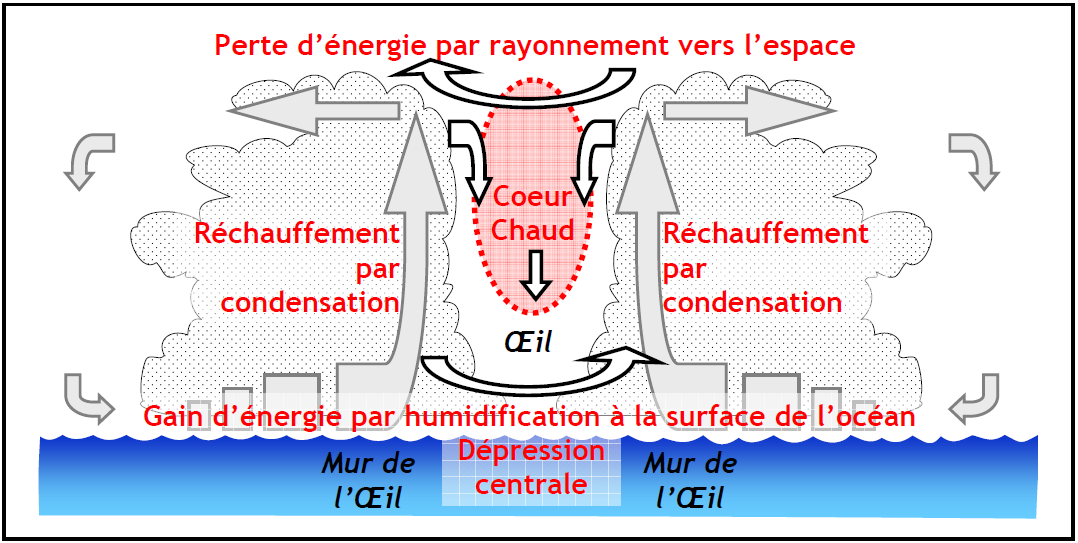
\includegraphics[width=\textwidth]{Figures/cyclones1_fig3_Cycle-thermodynamique-cyclone.png}
                \caption{Cycle thermodynamique d'un cyclone tropical à maturité\\
                \textit{Illustration de Frank Roux pour l'Encylopédie de l'Environnement, 20 Septembre 2018}}
            \end{figure}
        \end{column}
        \begin{column}{0.5\textwidth}
           \setlength{\leftmargini}{2.5ex}
           \vspace{-2em}
           \begin{block}[Grandeurs caractéristiques] 
                \footnotesize
                \begin{itemize}
                    \item Fréquence annuelle moyenne : 84 TC par an \mbox{\parencite{schreck_impact_2014}}
                    \item Diamètre moyen de l'œil : 55 \sim~85 km \mbox{\parencite{weatherford_typhoon_1985}}
                    \item Diamètre\footnotemark~total moyen: 500 km \parencite{carrasco_influence_2014}
                    \item Vitesse de déplacement moyenne : 20 km/h
                    \item Vents soutenus : Entre 120 et 300 km/h
                \end{itemize}
            \end{block}
        \end{column}
    \end{columns}
    \footnotetext{Basé sur la mesure ROCI (\textit{Radius of Outermost Closed Isobar})}
    \renewcommand*{\thefootnote}{\arabic{footnote}}
    \setcounter{footnote}{0}
\end{frame}

%===================================================
\begin{frame}[c]
    \frametitle{Qu'est-ce qu'un cyclone tropical ?}
    \framesubtitle{Bassins d'activité et classification}
    \begin{columns}
        \begin{column}{0.65\textwidth}
            \begin{figure}[h]
                \centering
                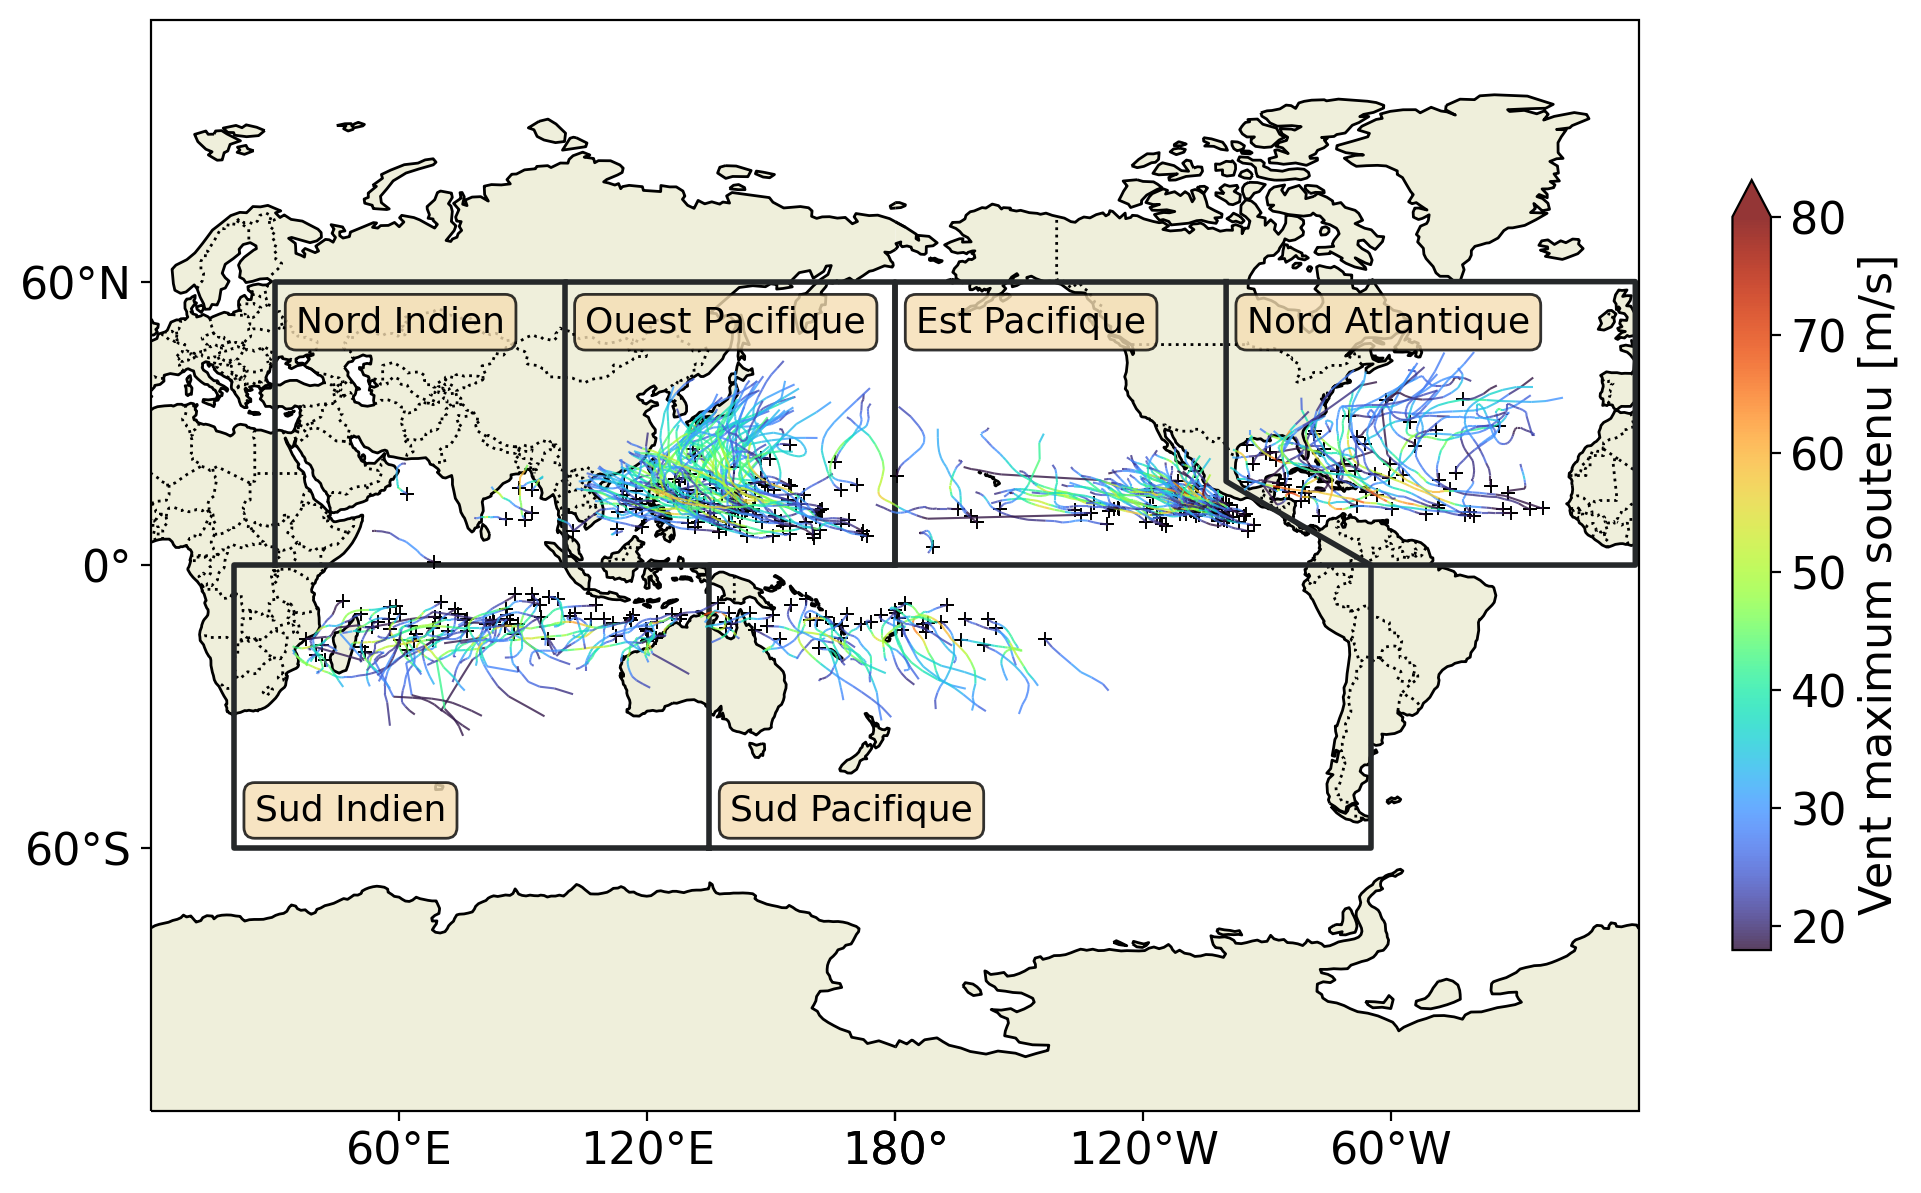
\includegraphics[width=\textwidth]{Figures/Bassins_et_trajectoires_soutenance.png}
                \caption{Données issues de la basé de données de cyclones IBTrACS, version 4}
            \end{figure}
        \end{column}
        \begin{column}{0.35\textwidth}
            \begin{table}[h]
                \centering
                \caption{Seuils de vents (sur 10 minutes) des catégories Saffir-Simpson (gauche) et seuils de pression équivalents ajustés
                selon \cite{klotzbach_surface_2020}.}
                \footnotesize
                \begin{tabular}{l|c|c}
                     & Vent (m/s) & Pression (hPa) \\
                    \hline
                    TD & $<$ 16 & $>$ 1005 \\
                    TS & 16 -- 28 & 1005 -- 991 \\
                    Cat 1 & 29 -- 37 & 990 -- 976 \\
                    Cat 2 & 38 -- 43 & 975 -- 961 \\
                    Cat 3 & 44 -- 51 & 960 -- 946 \\
                    Cat 4 & 52 --  62 & 945 -- 926\\
                    Cat 5 & $\geq$ 63 & $\leq$ 925
                \end{tabular}
            \end{table}
        \end{column}
    \end{columns}
\end{frame}

%===================================================
\begin{frame}[c]
    \frametitle{Qu'est-ce qu'un cyclone tropical ?}
    \framesubtitle{Conditions de formations}
    \begin{figure}[h]
        \centering
        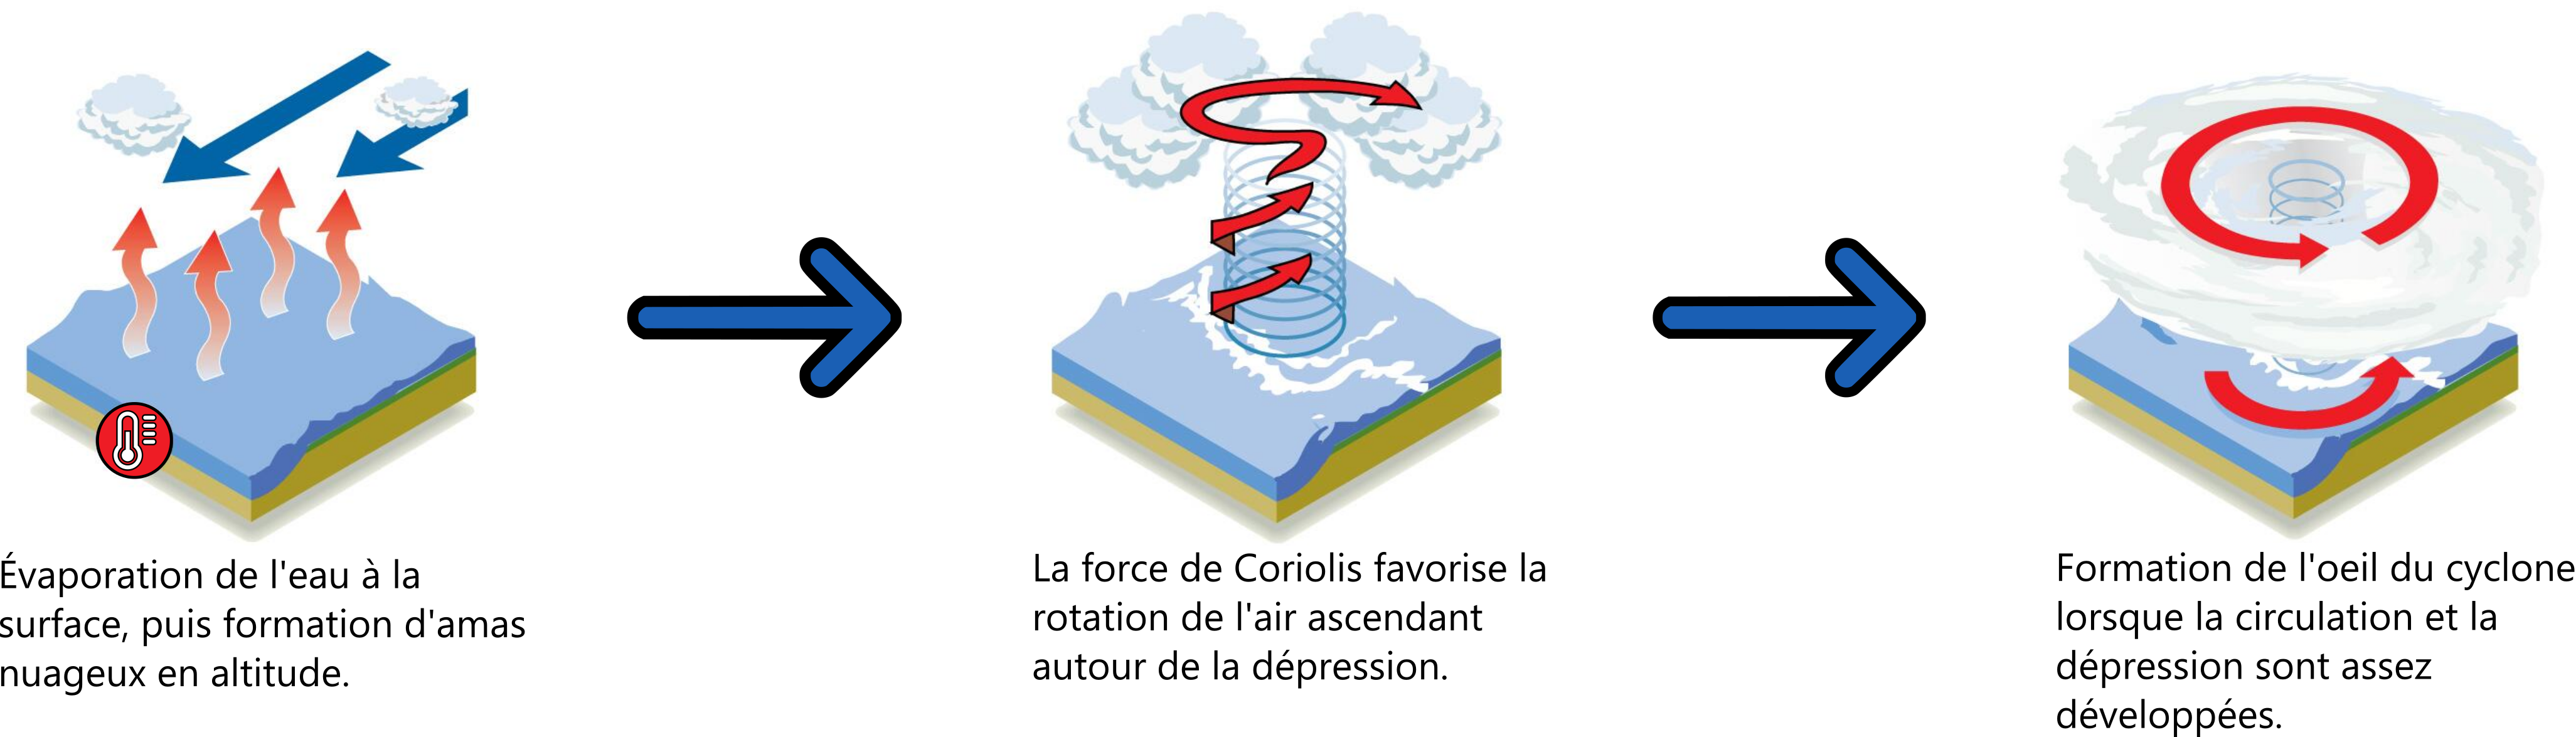
\includegraphics[width=0.8\textwidth]{Figures/diagramme_formation.png}
    \end{figure}
    %\vspace{1em}
    \footnotesize
    \begin{block}[Ingrédients de la cyclogénèse]
        \begin{columns}[t]
            \scriptsize
            \begin{column}{0.5\textwidth}
                \begin{itemize}
                   \item Perturbation initale apportant de la convergence en basses couches
                   \item Une distance de quelques centaines de kilomètres à l'équateur (Coriolis)
                   \item Température de surface de l'ocean supérieure à 26°C sur au moins 60m de profondeur \parencite{palmen_formation_1948}
                \end{itemize}
            \end{column}
            \begin{column}{0.5\textwidth}
               \begin{itemize}
                   %\setlength{\leftmargini}{1.5ex}
                   \item Absence de cisaillement vertical du vent\\\parencite{gray_global_1968}
                   \item Atmosphère humide en moyenne troposphère
                   \item Atmosphère instable
               \end{itemize} 
            \end{column}
        \end{columns}
    \end{block}
    \blfootnote{Illustration adaptée d'une infographie AFP existante}
\end{frame}

%===================================================
\begin{frame}[c]
    \frametitle{Qu'est-ce qu'un cyclone tropical ?}
    \framesubtitle{Le phénomène météorologique le plus destructeur}
    \begin{definition}
        \footnotesize
        \begin{itemize}
            \item Plus de 400 000 morts et près de 300 000 blessés entre 1980 et 2009 \parencite{doocy_human_2013}.
            \item 20 millions de personnes rendues sans-abri \parencite{doocy_human_2013}.
            \item Coût économique moyen de plus de 20 milliards de dollars par cyclone (TC) aux États-Unis \parencite{smith_billiondollar_2020}.
        \end{itemize} 
    \end{definition}
    \begin{columns}
        \begin{column}{0.45\textwidth}
            \begin{figure}[h]
                \centering
                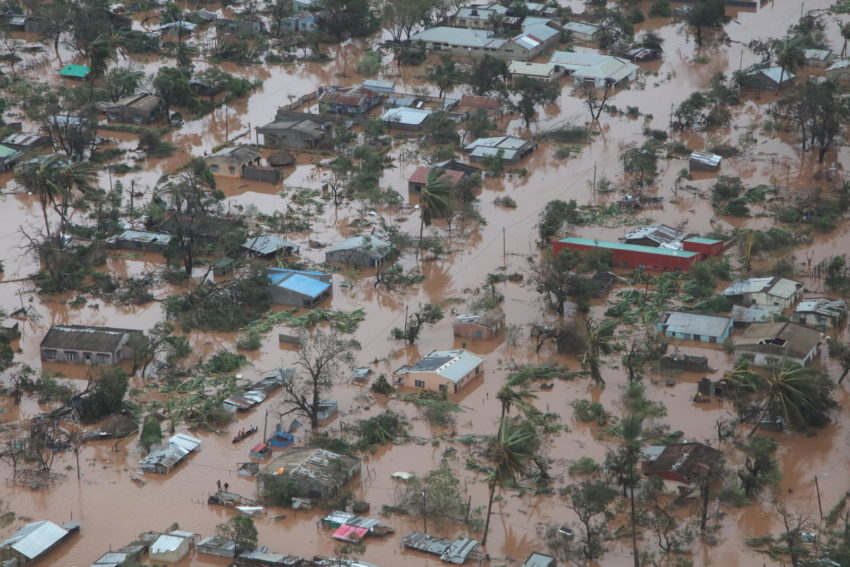
\includegraphics[width=0.97\textwidth]{Figures/idai_2019_sofala_province.jpg}
                \caption{Povince de Sofala au Mozambique après le passage du \mbox{cyclone} Idai, Mars 2019. \textit{Photo de l'Institut National
                de Gestion des Catastrophes du Mozambique (INGC).}}
            \end{figure}
        \end{column}
        \begin{column}{0.45\textwidth}
             \begin{figure}[h]
                 \centering
                 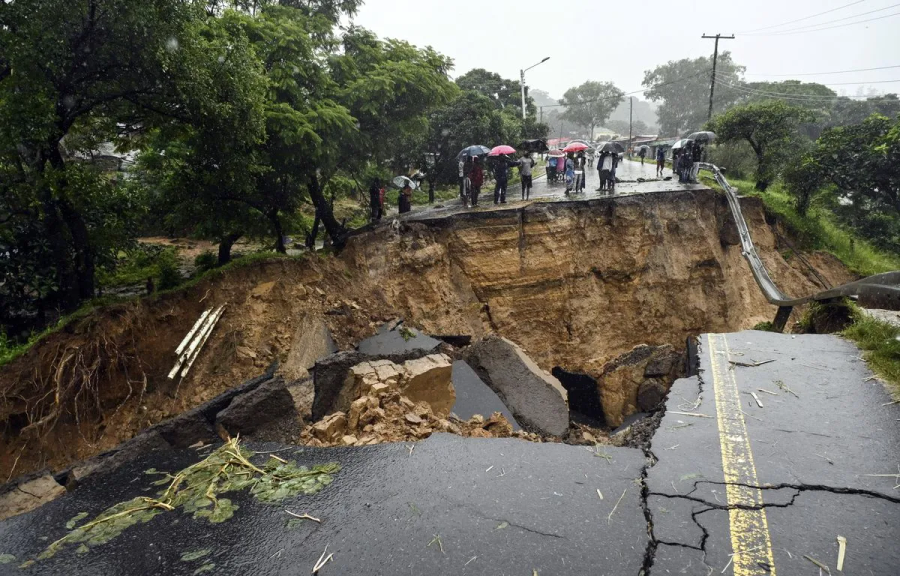
\includegraphics[width=\textwidth]{Figures/freddy_malawi_route.png}
                 \caption{Route endommagée au Malawi après le passage du cyclone Freddy, Mars 2023.\\\textit{Photo AP/SIPA/Thoko Chikondi}}
             \end{figure}
        \end{column}
    \end{columns}
\end{frame}

\subsection{Consensus sur les projections futures}

%=========================================================
\begin{frame}[c]
    \frametitle{Consensus sur l'évolution future de l'activité cyclonique}
    \begin{columns}
        \begin{column}{0.75\textwidth}
            \begin{figure}
                \centering
                \begin{tikzpicture}
                    \node<1->[anchor=south west, inner sep=0] (image) at (0,0)%
                        {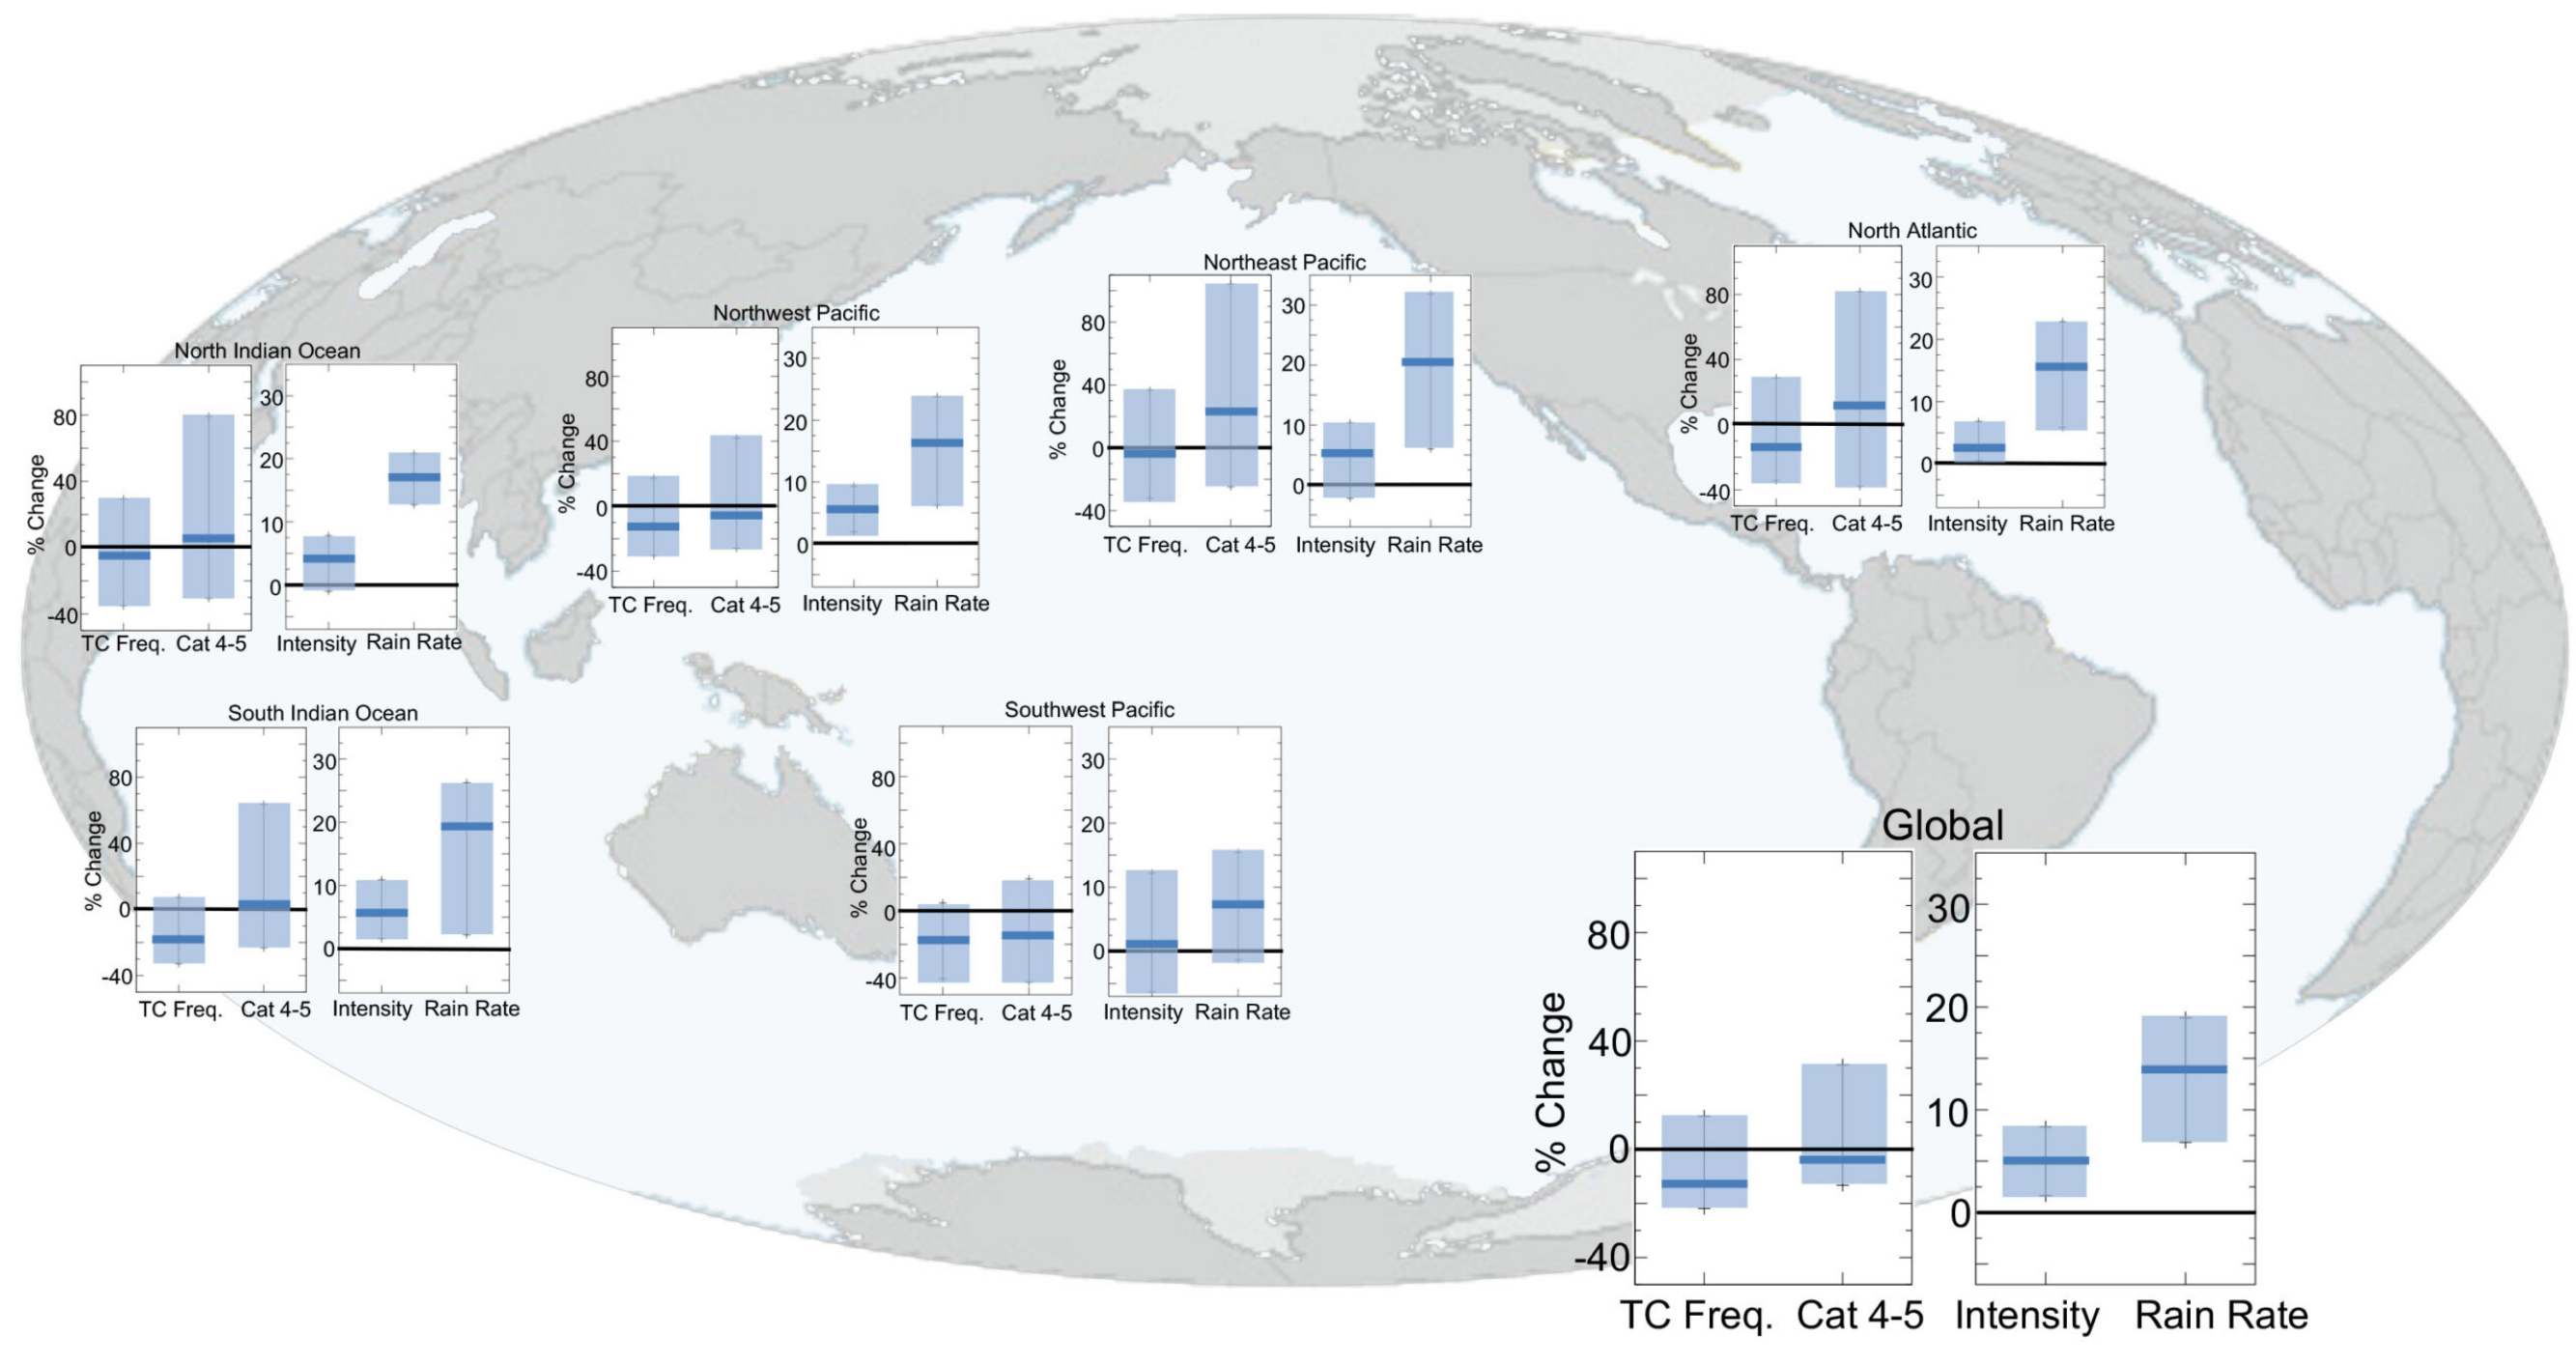
\includegraphics[width=\textwidth]{Figures/Fig_5_Knutson_BAMS_revised_3_9_20-scaled_cropped.png}};
                    \begin{scope}[x={(image.south east)},y={(image.north west)}]
                        \draw<2->[rounded corners=0.5mm, red, fill, fill opacity=0.1, line width=0.5] (0.627, 0.018) rectangle (0.69, 0.055);
                        \draw<3->[rounded corners=0.5mm, green, fill, fill opacity=0.1, line width=0.5] (0.6955, 0.018) rectangle (0.749, 0.055);
                        \draw<4->[rounded corners=0.5mm, blue, fill, fill opacity=0.1, line width=0.5] (0.755, 0.018) rectangle (0.818, 0.055);
                        \draw<5->[rounded corners=0.5mm, purple, fill, fill opacity=0.1, line width=0.5] (0.825, 0.018) rectangle (0.898, 0.055);
                    \end{scope}
                \end{tikzpicture}
                \caption{Synthèse des projections de l'activité cyclonique pour un réchauffement de 2°C par rapport à 1986 -- 2005
                \parencite{knutson_tropical_2020}. Médianes et intervalles de confiance de respectivement 90~\% et 80~\% (gauche et droite).}
            \end{figure}
        \end{column}
        \begin{column}{0.25\textwidth}
           \footnotesize
           \setlength{\leftmargini}{2.5ex}
           \onslide<2->{
               \begin{block}[Résumé]
                   \scriptsize
                   \begin{itemize}
                        \item<2-> \textcolor{red}{Fréquence toutes catégories} : Baisse probable
                        \item<3-> \textcolor{green}{Fréquence des cyclones forts} : Hausse \underline{relative}
                        \item<4-> \textcolor{blue}{Intensité maximale} : Hausse fortement probable
                        \item<5-> \textcolor{purple}{Précipitations} : Hausse très fortement probable
                   \end{itemize}
               \end{block}
           }
           \onslide<6->{
               \begin{alertblock}
                    \scriptsize
                    Incertitudes conséquentes, y compris parfois sur le signe du changement
               \end{alertblock}
           }
        \end{column}
    \end{columns}
\end{frame}

\subsection[Méthodologies d'évaluation]{Comment sont réalisées ces projections ?}
\makesubsecslide

%=========================================================
\begin{frame}[c]
    \frametitle{Les modèles de climat}
    \framesubtitle{Simulation numérique de l'évolution de l'état de l'atmosphère}
    \begin{columns}
        \begin{column}{0.55\textwidth}
            \footnotesize
            \begin{definition} 
                Discrétisation des équations régissant l'évolution de l'état de \mbox{l'atmosphère} dans le temps et \alert{l'espace}\\
                $\longrightarrow$ ~L'échelle de la \alert{maille}
            \end{definition}
            \vspace{1em}%
            \onslide<2->{
                \begin{block}[Résolutions horizontales des modèles actuels \parencite{ipcc_annex_2021}]
                    \begin{itemize}
                        \item Hautes résolutions : 20 \sim~80 km
                        \item Basses résolutions : 100 \sim~250 km
                    \end{itemize}
                \end{block}
            }
            \vspace{1em}%
            \onslide<3->{
                \begin{alertblock}
                    On commence tout juste à pouvoir descendre à l'échelle nécessaire pour simuler des TC \underline{réalistes} aux échelles de temps
                    climatiques
                \end{alertblock}
            }
        \end{column}
        \onslide<1->{
            \begin{column}{0.45\textwidth}
                \begin{figure}[t]
                    \centering
                    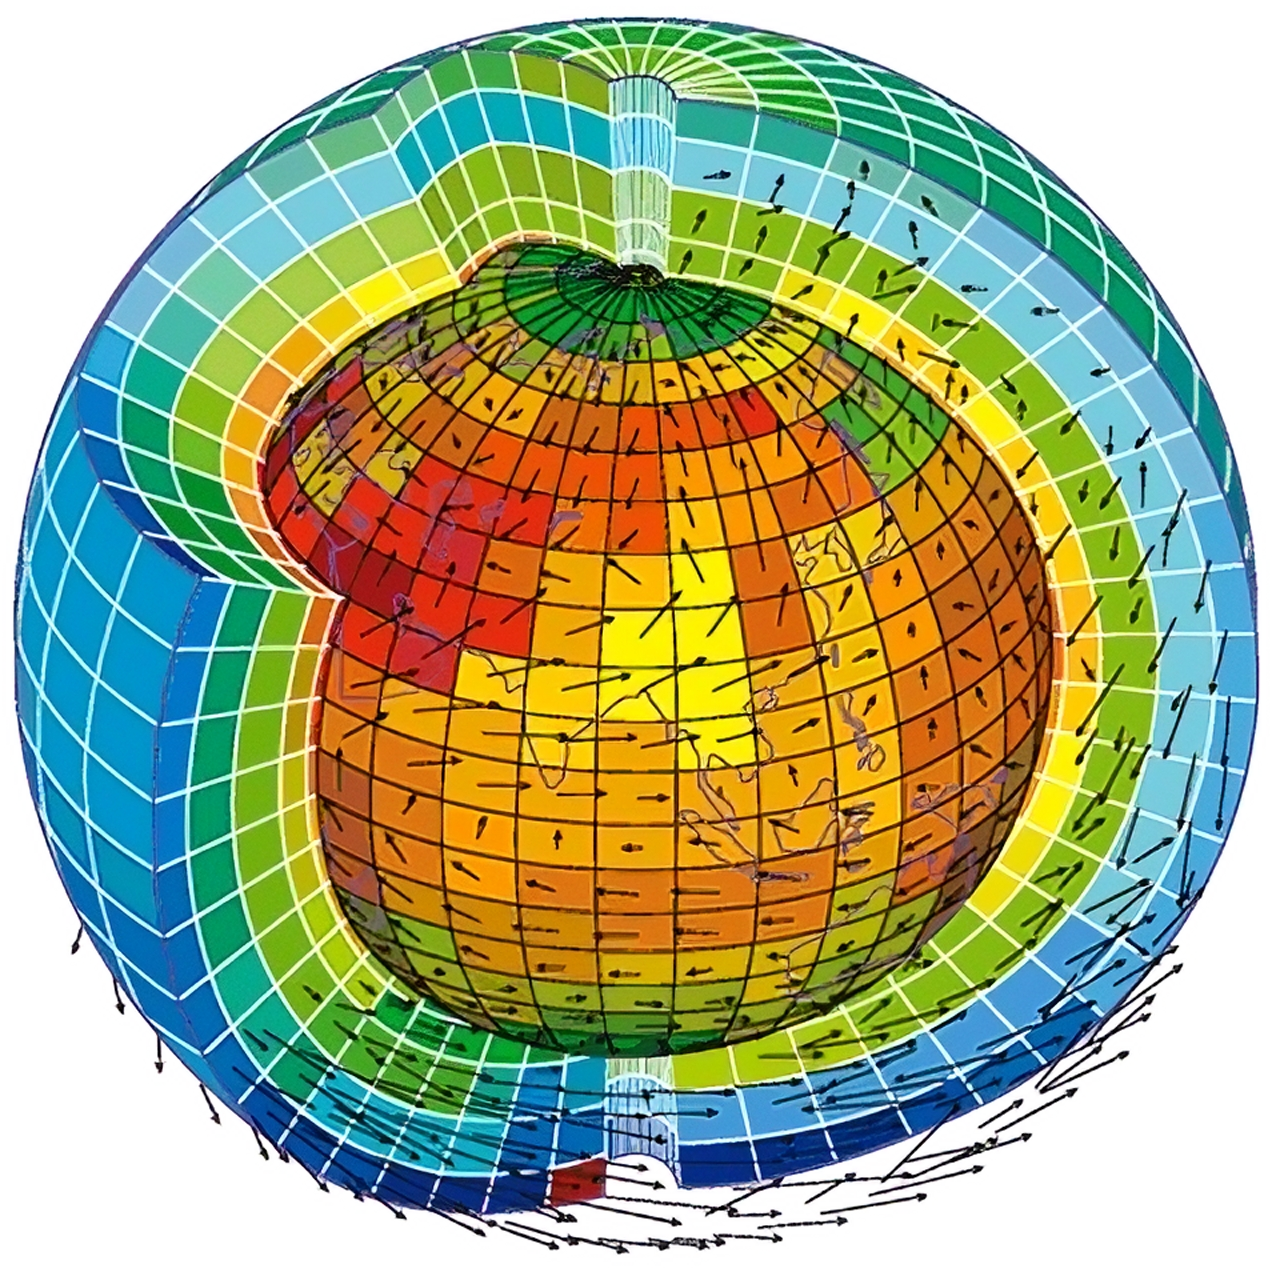
\includegraphics[width=0.8\textwidth]{Figures/maillage_upscaled_x4_2.png}
                    \captionsetup{width=0.9\textwidth}
                    \caption{Illustration schématique du maillage tridimensionnelle d'un modèle de climat. Les couleurs représentent la température et les flèches
                    le vent.\\\textit{Illustration de \mbox{Laurent Fairhead/LMD/CNRS}}.}
                \end{figure}
            \end{column}
        }
    \end{columns} 
\end{frame}

%=========================================================
\begin{frame}
    \frametitle{Les réanalyses atmosphériques}
    \framesubtitle{Simulation numérique de l'état passé de l'atmosphère}
    \begin{columns}[c]
        \begin{column}{0.5\textwidth}
            \footnotesize
            \begin{block}
                \begin{itemize}
                \setlength\itemsep{3.5ex}
                    \item \alert{Reconstruction} spatiale (3D) et temporelle de l'état passé de l'atmosphère
                    \item Versions figées du modèle et du schéma d'assimilation\\
                        $\longrightarrow$ Jeu de données \alert{complet} et \alert{cohérent} dans le temps et l'espace
                    \item Souvent utilisées comme proxy d'observations \textit{in-situ}
                \end{itemize}
            \end{block}
        \end{column}
        \begin{column}{0.5\textwidth}
            \vspace{-2em}
            \begin{figure}
                \centering
                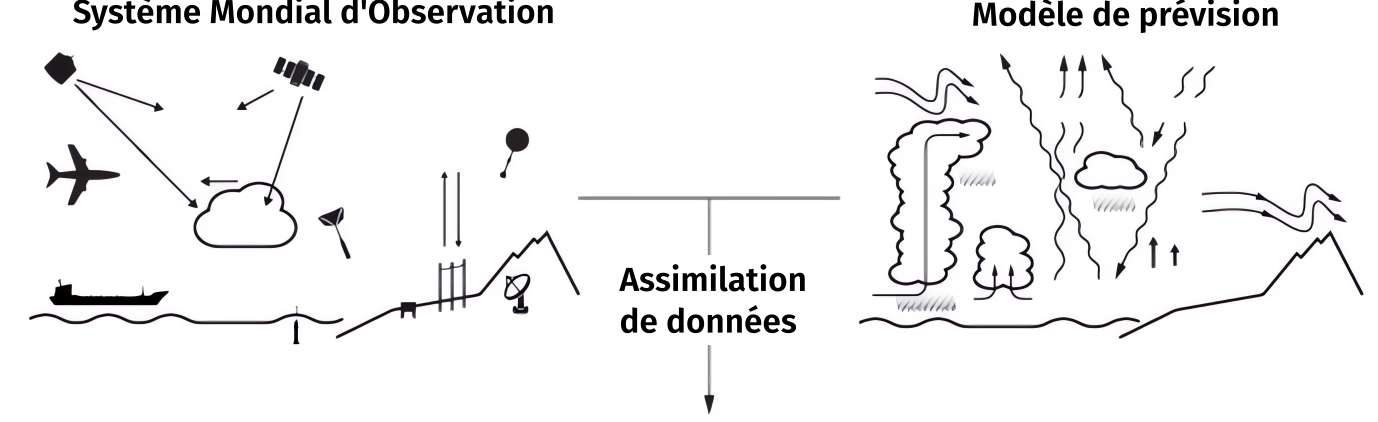
\includegraphics[width=\textwidth]{Figures/schema_reanalyse_top_custom.png}
                \animategraphics[autoplay,loop,width=\textwidth,poster=59]{13}{Figures/u850_octobre_2017/frame.00}{000}{123}
                \caption{Principe de fonctionnement de la réanalyse atmosphérique.\\Vent zonal à 850 hPa pour Octobre 2017 (ERA5).\\\textit{Adapté d'une illustration du CEPMMT (ECMWF)}}
            \end{figure} 
        \end{column}
    \end{columns} 
    %
    \begin{center}
        \begin{minipage}{12cm}
            \begin{definition}
                \centering
                \small
                Les réanalyses font le lien entre les sorties des modèles de climat et les observations
            \end{definition}
        \end{minipage}
    \end{center}
\end{frame}

%=========================================================
\begin{frame}[c]
    \frametitle{1\iere~approche : Détection et suivi objectif}
    \framesubtitle{Mesure directe dans les simulations haute résolution}
    \begin{columns}
        \begin{column}{0.66\textwidth}
            \footnotesize
            \begin{definition}
                \centering
                Algorithmes identifiant et reliant entre eux les points de grille qui satisfont une ou plusieurs conditions.
            \end{definition}
            \vspace{1em}
            \onslide<2->{
                \begin{block}
                    \centering
                    Statistiques descriptives sur le nombre et les propriétés des cyclones détectés dans des simulations en climat futur
                \end{block}
            }
            \begin{columns}[t]
                \setlength{\leftmargini}{2.5ex}
                \begin{column}{0.45\textwidth}
                    \onslide<3->{
                        \begin{examples}[Intérêt principal]
                            \scriptsize
                            Mesure \alert{directe}
                            \tcblower
                            \scriptsize
                            \begin{itemize}
                                \item Capture le cycle de vie et la structure spatiale des cyclones
                                \item Permet une évaluation de tous les aspects de l'activité cyclonique
                            \end{itemize}
                        \end{examples}
                    }
                \end{column}
                \begin{column}{0.45\textwidth}
                    \onslide<4->{
                        \begin{alertblock}[Inconvénients] 
                            \scriptsize
                            \begin{itemize}
                                \item Nécessite des simulations à haute résolution (\alert{coûteuses} et encore trop \alert{peu nombreuses})
                                \vspace{2.9ex}
                                \item Sensibilité à la méthodologie de détection \parencite{horn_tracking_2014,bourdin_intercomparison_2022}
                            \end{itemize}
                        \end{alertblock}
                    }
                \end{column}
            \end{columns}
            %\vspace{1em}
        \end{column}
        %
        \onslide<1->{
                \begin{column}{0.33\textwidth}
                \captionsetup{width=4cm}
                \vspace{-3em}
                \begin{figure}
                    \centering 
                    \animategraphics[autoplay,loop,width=4cm,poster=22]{5}{Figures/Ophelia/vo850/ophelia-vo850-}{0}{27}
                    \caption{\href{run:./ophelia-vo850.gif}{Animation} du cyclone Ophelia (2017) sur fond de \alert{vorticité relative à 850 hPa} (ERA5)}
                \end{figure}
                %
                \begin{figure}
                    \centering
                    \animategraphics[autoplay,loop,width=4cm,poster=22]{5}{Figures/Ophelia/msl/ophelia-msl-}{0}{27}
                    \caption{\href{run:./ophelia-msl.gif}{Animation} du cyclone Ophelia (2017) sur fond de \alert{pression au niveau de la mer} (ERA5)}
                \end{figure}
            \end{column}
        }
    \end{columns}
\end{frame}

%=========================================================
\begin{frame}[t]
    \frametitle{2\ieme~ approche : Indices de cyclogénèse}
    \framesubtitle{Inférence de l'activité par l'environnement de grande échelle}
    \begin{columns}[t]
        \begin{column}{0.5\textwidth}
            \begin{definition}
                \scriptsize
                %\centering
                \underline{Fréquence d'occurrence} des TC en un point de grille proportionnelle à une \mbox{combinaison} de variables \alert{thermiques} et
                \mbox{\alert{dymamiques}} de grande échelle \parencite{gray_tropical_1975}.
            \end{definition}
            \onslide<2->{
                \vspace{1em}
                \begin{block}
                    \scriptsize
                    \centering
                    %Relations établies en climat présent pour application à des simulations en climat futur.
                    Relations caractérisant la climatologie spatio-temporelle présente, et appliquées à des simulations en climat futur.
                \end{block}
            }
            \begin{columns}[t]
                \setlength{\leftmargini}{2ex}
                \begin{column}{0.45\textwidth}
                    \onslide<3->{
                        \footnotesize
                        \begin{examples}[Intérêt principal]
                            \scriptsize
                            Applicable à des modèles basse résolution\\(plus nombreux \Rightarrow Meilleure estimation de l'incertitude)
                        \end{examples}
                    }
                \end{column}
                \begin{column}{0.45\textwidth}
                    \onslide<4->{
                        \footnotesize
                        \begin{alertblock}[Inconvénients]
                            \scriptsize
                            \begin{itemize}
                                \item Mesure \alert{indirecte}
                                \vspace{1ex}
                                \item Incertitudes sur le choix des variables
                            \end{itemize}
                        \end{alertblock}
                    }
                \end{column}
            \end{columns}
        \end{column}
        \begin{column}{0.5\textwidth}
            \vspace{-3em}
            \begin{figure}
                \centering
                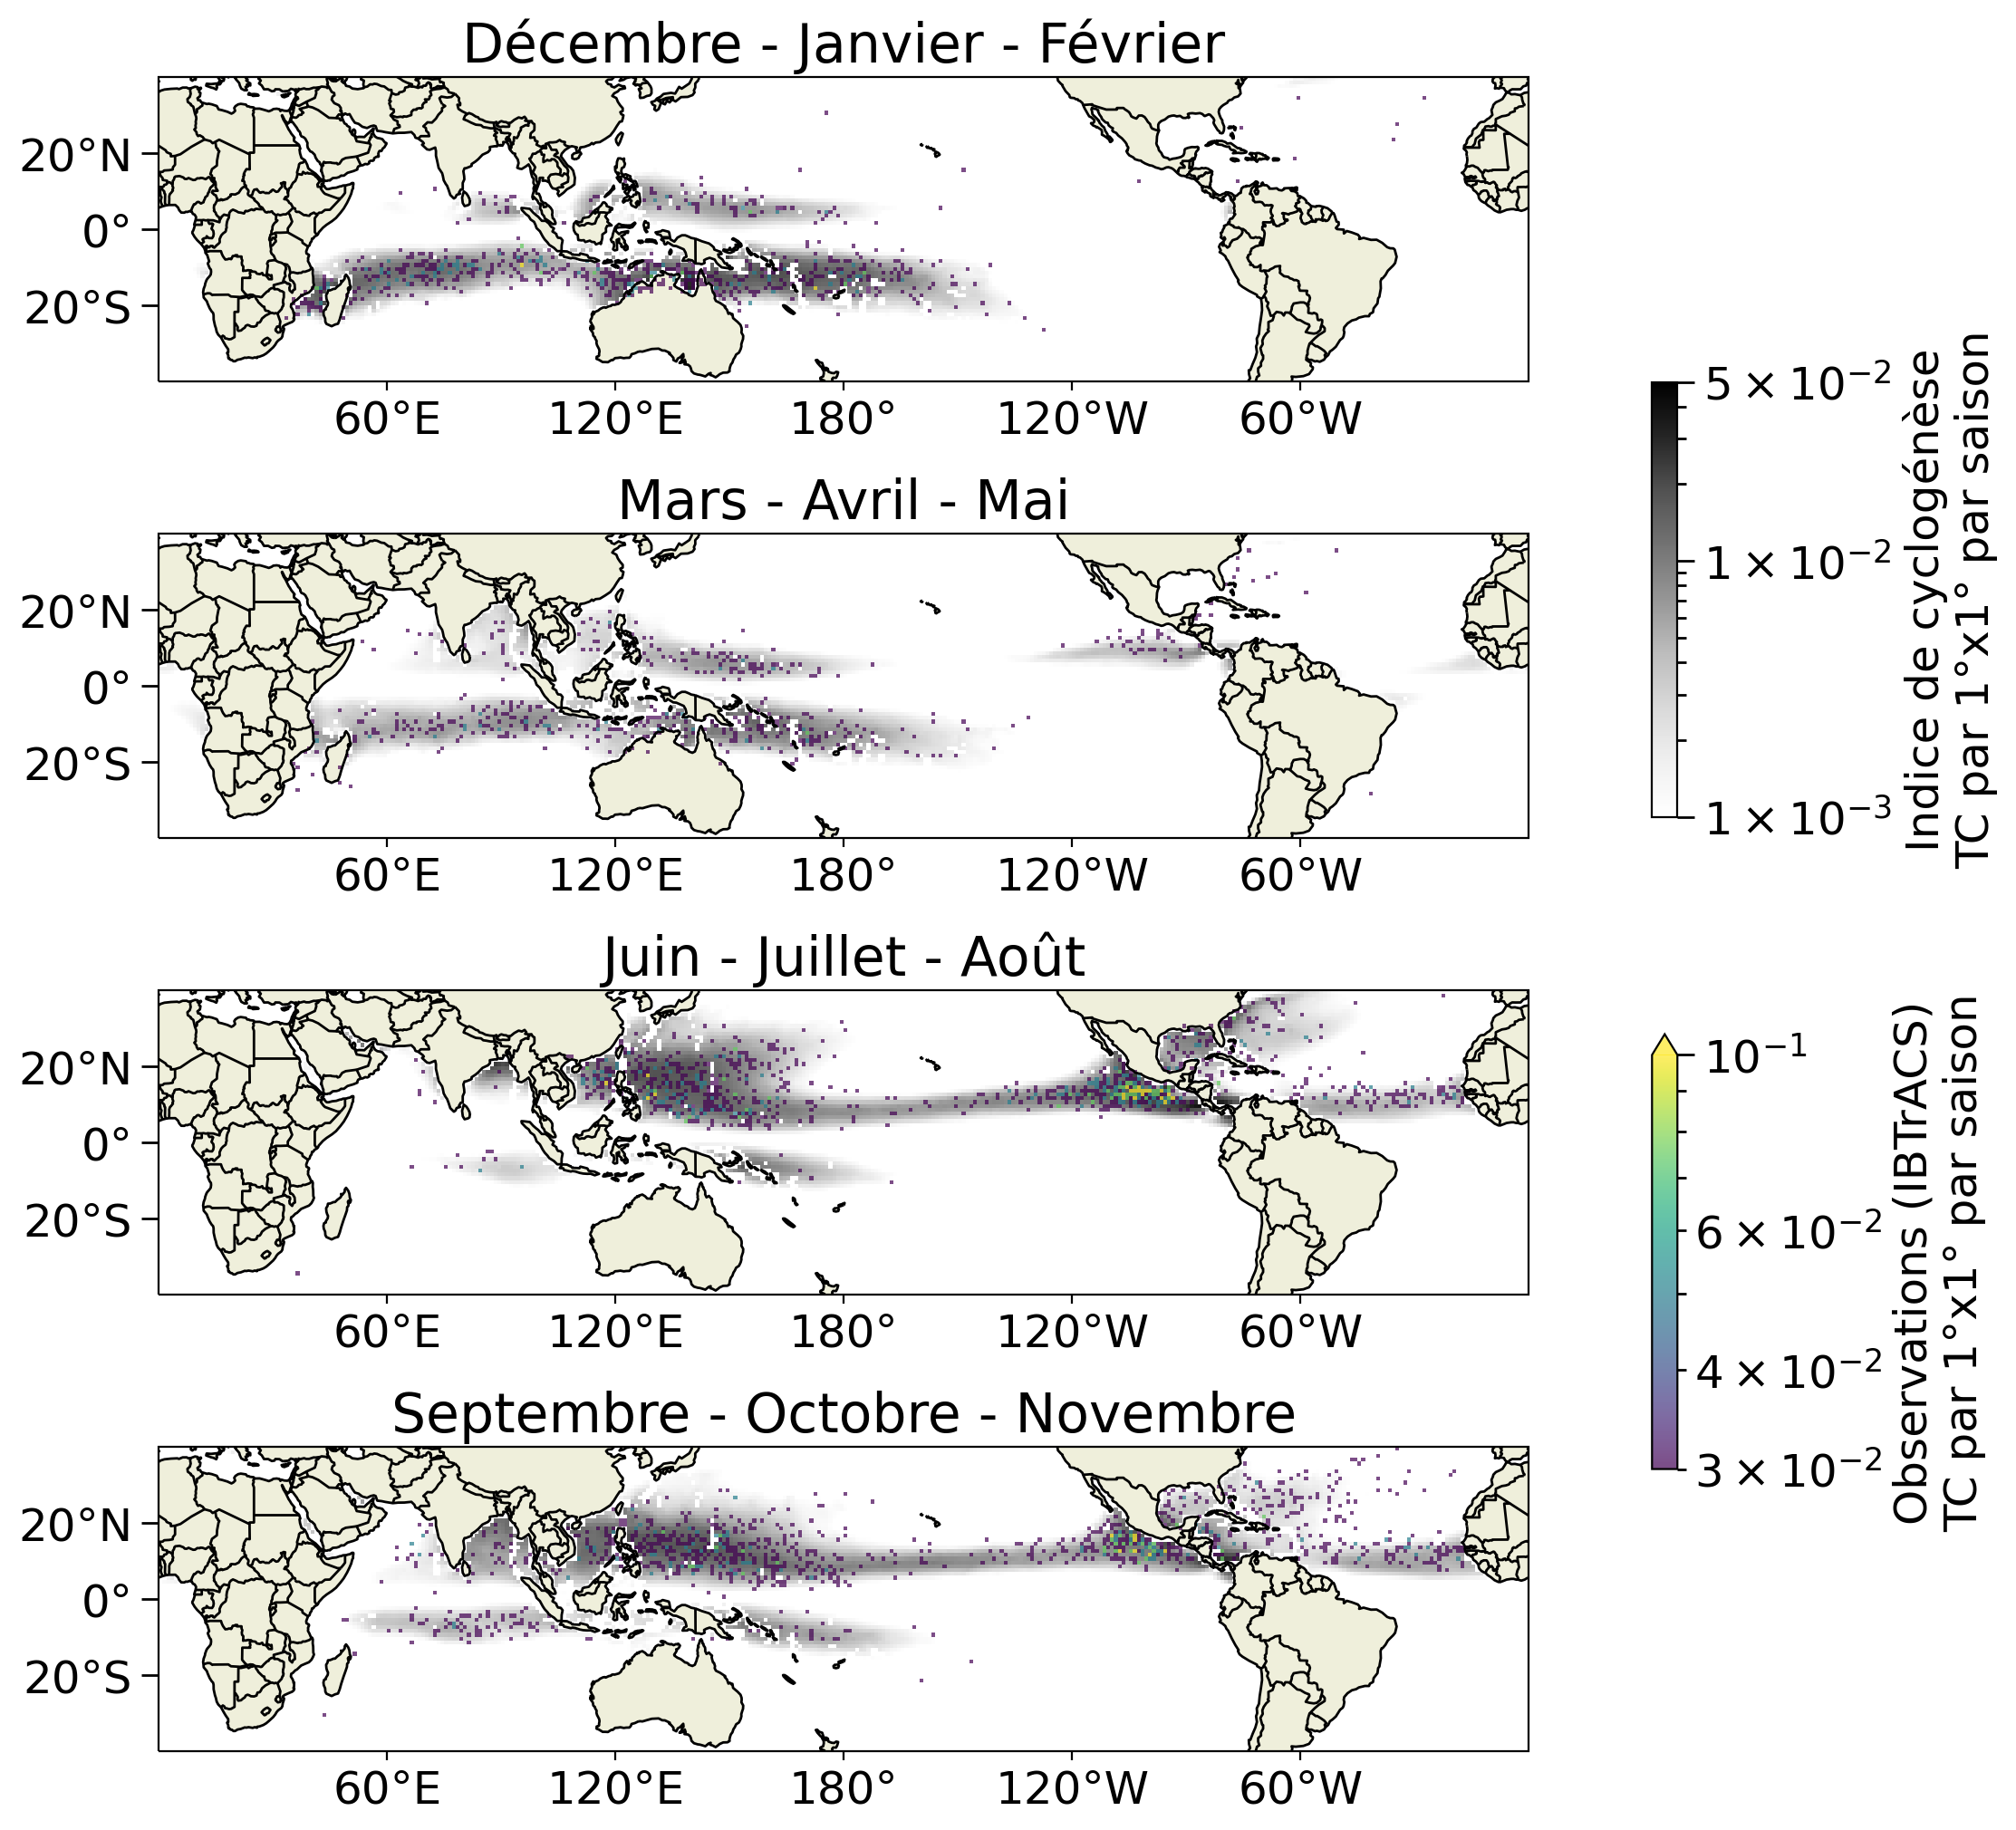
\includegraphics[width=\textwidth]{Figures/acgi_mean_IBTrACS_season.png}
                \caption{Moyennes saisonnières de trois indices moyennés entre eux (GPI, TCS et CYGP), et densité observée de cyclogénèse entre 1980 et 2019
                (IBTrACS).}
            \end{figure}        
        \end{column}
    \end{columns}
\end{frame}

%=========================================================
\subsection{Problématique}
\begin{frame}[t]
    \frametitle{Problématique}
    \framesubtitle{Contexte général}
    \vspace{-1em}
    \begin{columns}[b]
        \begin{column}{0.5\textwidth}
            \begin{figure}[h]
                \centering
                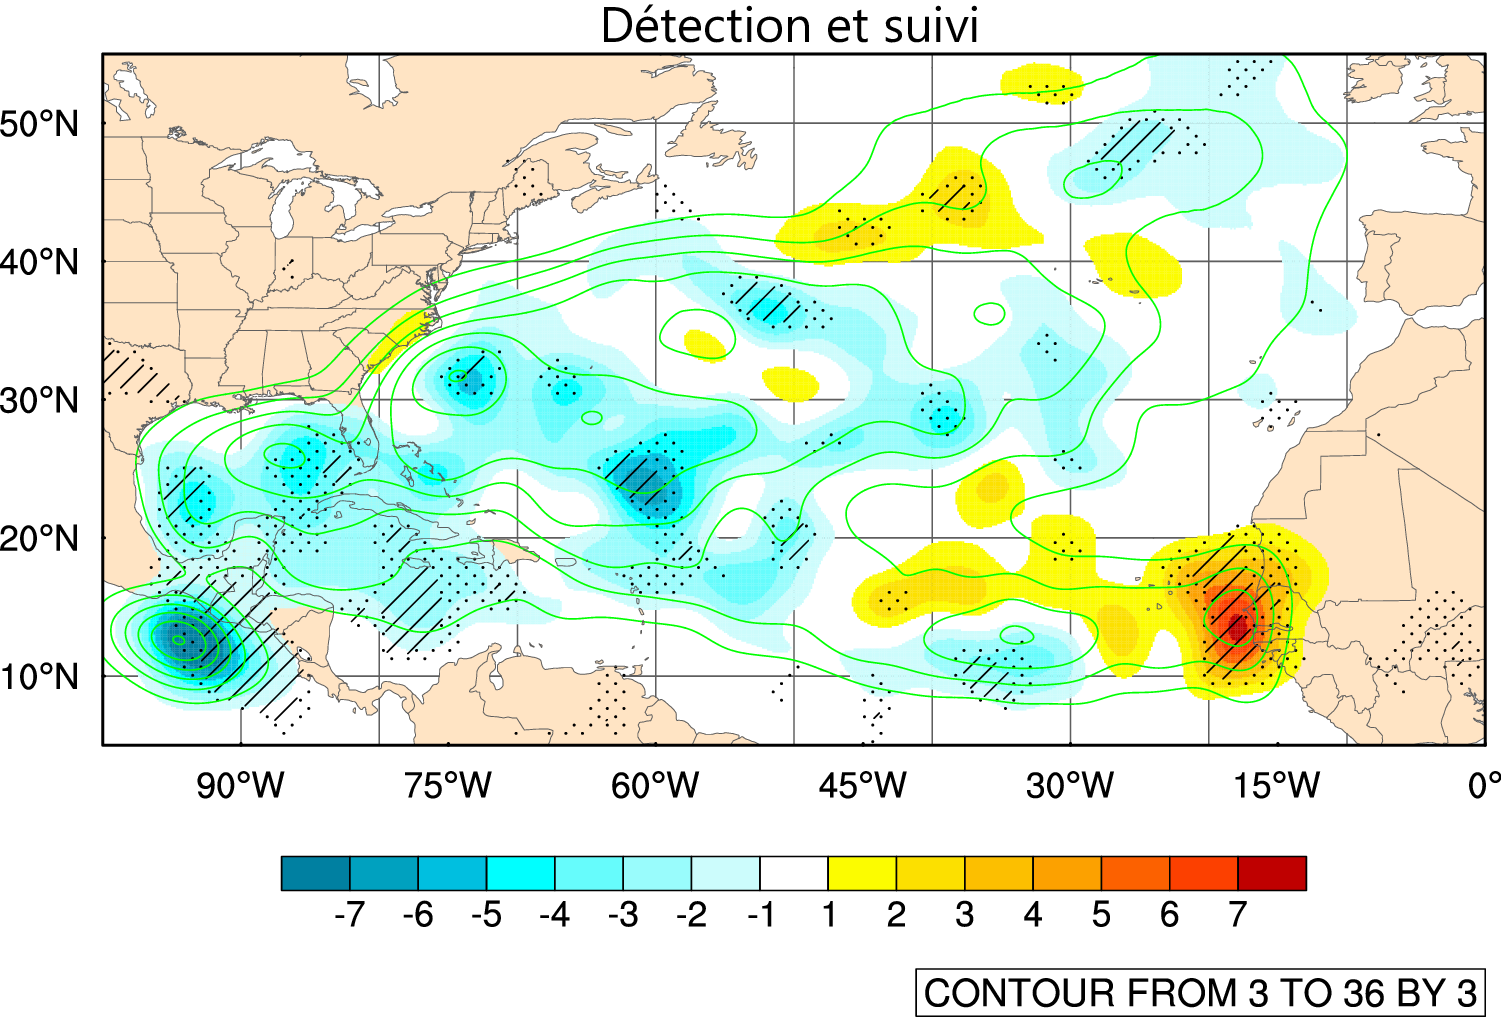
\includegraphics[width=\textwidth]{Figures/density_fitted_title.png}
                \caption{Changement dans la densité de cyclogénèse (par 50 ans) par mesure \alert{directe} sur la période 2031 -- 2080 (RCP 8.5) par rapport à 1965 -- 2013
                \parencite{chauvin_future_2020}}
            \end{figure}
        \end{column}
        \begin{column}{0.5\textwidth}
            \begin{figure}[h]
                \centering
                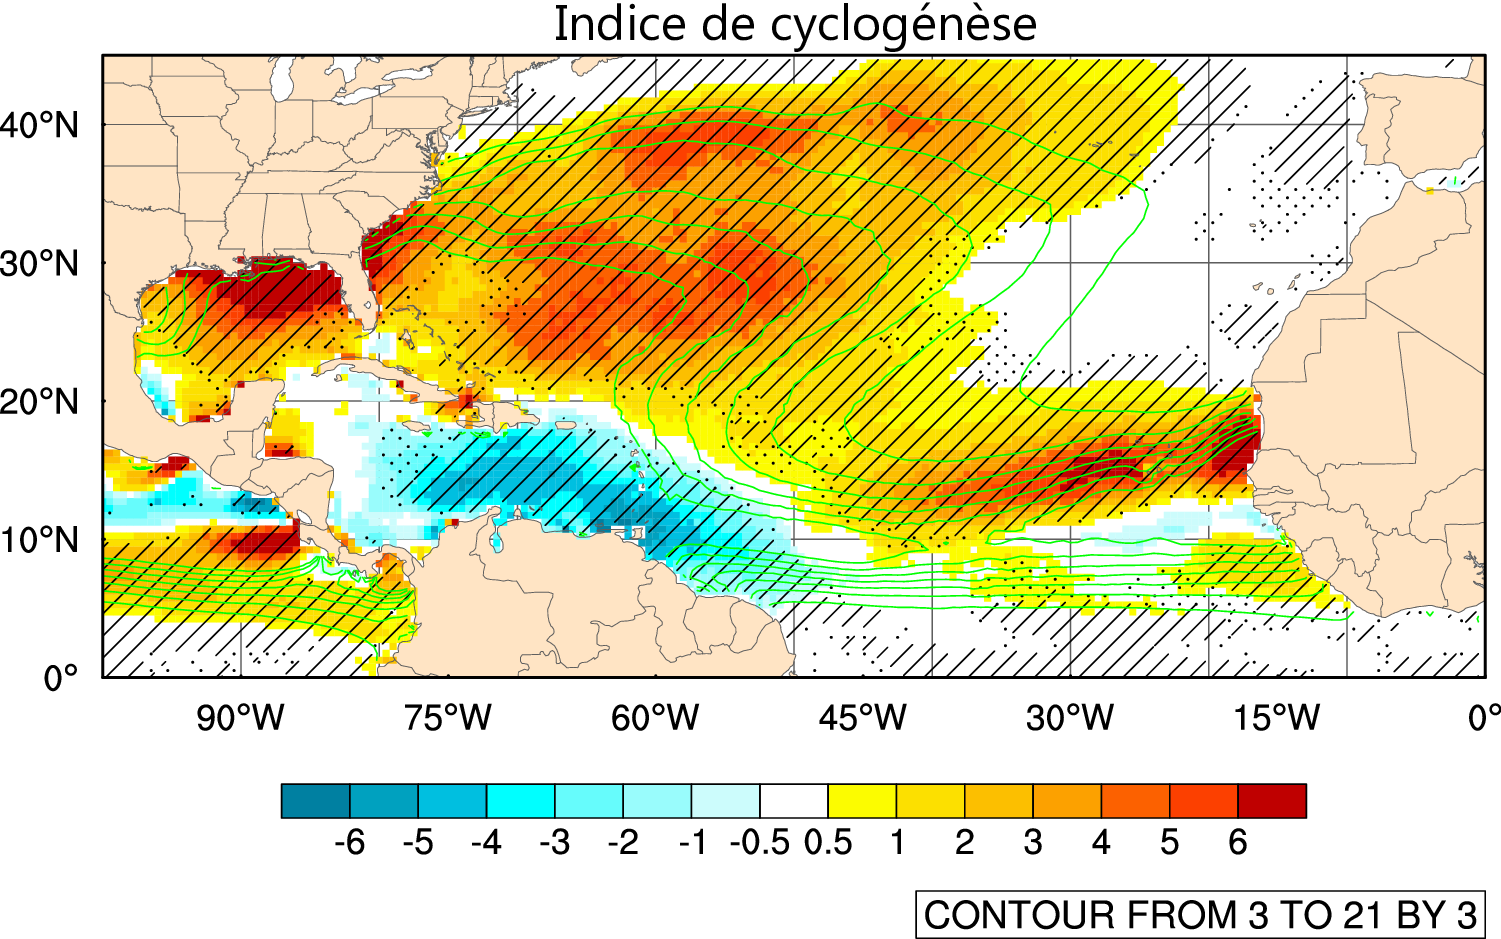
\includegraphics[width=\textwidth]{Figures/gpi_fitted_2_good_title.png}
                \caption{Changement dans la densityé de cyclogénèse (par 50 ans) par mesure \alert{indirecte} (GPI) sur la période 2031 -- 2080 (RCP 8.5) par
                rapport à 1965 -- 2013}
            \end{figure}
        \end{column}
    \end{columns}
    %
    \onslide<2->{
        \begin{center}
            \begin{minipage}{4.5cm}
                \begin{alertblock}
                    \centering
                    \footnotesize
                    Les projections \underline{\alert{divergent}}
                \end{alertblock}
            \end{minipage}
        \end{center}
    }
\end{frame}

%=========================================================
%\begin{frame}
%    \frametitle{Problématique}
%    \framesubtitle{Recherches menées}
%    2 colones :
%    \begin{itemize}
%        \item Hypothèse de la variabilité interannuelle (indices)
%        \item Qu'est-ce qu'on détecte vraiment avec un traqueur (tracking)
%    \end{itemize}
%    
%\end{frame}

\begin{frame}[t]
    \frametitle{Problématique}
    \framesubtitle{Recherches menées}
    \vspace{-2em}
    \begin{columns}[t]
        \begin{column}{0.475\textwidth}
            \onslide<1->{
                \begin{center}
                    \large
                    \textbf{Détection et suivi} 
                \end{center}
            }
            \vspace{0.8em}
            \footnotesize
            \onslide<2->{
                \begin{alertblock}[Verrous identifiés]
                    \setlength{\leftmargini}{2.5ex}
                    \begin{itemize}
                        \item Influence du choix du traqueur dans les projections \parencite{horn_tracking_2014} 
                        \item Qu'est-ce que détecte réellement un traqueur ?
                    \end{itemize}
                \end{alertblock}
            }
            \vspace{2em}
            \onslide<3->{
                \begin{examples}[Axe de recherche]
                    Caractériser en détails le schéma de détection du CNRM pour identifier des pistes de perfectionnement
                \end{examples}
            }
            \vspace{1em}
            \onslide<4->{
                $\longrightarrow$ Développement de métriques d'évaluation des performances d'un schéma de détection
            }
        \end{column}
        %
        \begin{column}{0.475\textwidth}
            \onslide<1->{
                \begin{center}
                    \large
                    \textbf{Indices de cyclogénèse} 
                \end{center}
            }
            \vspace{0.5em}
            \footnotesize
            \onslide<5->{
                \begin{alertblock}[Verrous identifiés]
                    \setlength{\leftmargini}{2.5ex}
                    \begin{itemize}
                        \item Tendances projetées à l'opposé de l'approche directe \parencite{camargo_testing_2014}
                        \item Mauvaise représentation de la variabilité interannuelle \parencite{menkes_comparison_2012,cavicchia_tropical_2023}
                    \end{itemize}
                \end{alertblock}
            }
            \vspace{1em}
            \onslide<6->{
                \begin{examples}[Hypothèse de travail]
                    Améliorer la variabilité interannuelle pour avoir une meilleure confiance dans les projections futures
                \end{examples}
            }
            \vspace{1em}
            \onslide<7->{
                $\longrightarrow$ Recherche de l'amélioration de la représentation de la variabilité interannuelle par les indices de cyclogénèse
            }
        \end{column}
    \end{columns}
\end{frame}



%=========================================================
\section[Détection et suivi]{Détection et suivi : Application du traqueur CNRM à la réanalyse ERA5}
\begin{frame}[c]
    \frametitle{Plan}
    \addtocounter{framesinsection}{-1}
    \tableofcontents[currentsection,hideallsubsections,sections={1-2}]
    \vspace{-3em}
    \tableofcontents[hideallsubsections,sections={3-}]
\end{frame}

\begin{frame}[c]
    \frametitle{Plan}
    \addtocounter{framesinsection}{-1}
    \tableofcontents[currentsection,hideothersubsections]
\end{frame}

%=========================================================
\subsection*{Motivations}
\begin{frame}[t]
    \frametitle{Introduction}
    \framesubtitle{Intérêts de la réanalyse ERA5}
    \onslide<1->{
        \begin{center}
            \begin{minipage}{10cm}
                \small
                \begin{definition}[Réanalyse ERA5 \parencite{hersbach_era5_2020}]
                    \footnotesize
                    \begin{itemize}
                        \item Dernière réanalyse en date du CEPMMT
                        \item Résolution horizontale $\sim$ 0.28° (25 km) sur tout le globe
                        \item De 1940 à aujourd'hui (en cours)
                    \end{itemize}
                \end{definition}
            \end{minipage}
        \end{center}
    }
    %
    \vspace{1.5em}
    %
    \begin{columns}[t]
        \begin{column}{0.5\textwidth}
            \onslide<2->{
                \small
                \begin{block}[Contexte de la thèse]
                    \footnotesize
                    Meilleure approximation de l'état \underline{historique} de l'atmosphère
                    \tcblower
                    \begin{itemize}
                        \footnotesize
                        \item La plupart des TC observés sont présents dedans
                        \item Permet la validation du schéma de détection
                    \end{itemize}
                \end{block}
            }
        \end{column}
        \begin{column}{0.5\textwidth}
            \onslide<3->{
                \small
                \begin{block}[Intérêt scientifique]
                    \begin{itemize}
                        \footnotesize
                        \item Produit de référence utilisé pour combler le manque entre les observations et les sorties de modèle 
                        \item Beaucoup d'attentes pour la représentation des TC en raison de sa haute résolution
                    \end{itemize}
                \end{block}
            }
        \end{column}
    \end{columns}
    % Slide d'introduction pour justifier le fait de travailler sur ERA5
    % \begin{itemize}
    %     \item Dans le contexte de la thèse : validation de l'outil de tracking
    %     \item Intérêt pour la communauté scientifique : \textquote{Nouveau} produit de référence, haute résolution, beaucoup d'espoir pour la représentation des
    %         TC.
    % \end{itemize}
\end{frame}

%=========================================================
\subsection{Données et outils}
\begin{frame}[t]
    \frametitle{Schéma de détection du CNRM}
    \footnotesize
    \begin{block}[Étapes de détection \parencite{chauvin_response_2006}] 
        \scriptsize
        \begin{enumerate}
            \item<1-> \textcolor[HTML]{ff0011}{Seuil} de vorticité (\textbf{VOR})
            \item<3-> Estimation de la taille du \textcolor{green}{système} \onslide<4->{et de son \textcolor{blue}{environnement}}
                \onslide<5->{
                    \begin{itemize}
                        \scriptsize
                        \item Seuil de vent à 10~m (\textbf{RES})
                        \item Anomalie de température cumulée à 700~hPa, 500~hPa et 300~hPa (\textbf{TANOM})
                        \item Profil vertical de température entre 300~hPa et 850~hPa (\textbf{PT})
                        \item Profil vertical de vent entre 300~hPa et 850~hPa (\textbf{PW})
                    \end{itemize}
                }
            \item<6-> Suivi du système (reliage des points)
            \item<7-> \textcolor{violet}{Relaxation} des paramètres pour \underline{compléter} en amont et en aval (\textbf{REL})
        \end{enumerate}
    \end{block}
    %\vspace{1em}
    \begin{figure}
        \centering
        \includegraphics<1>[height=2.8cm]{Figures/fonctionnement_tracker/step0.png}%
        \includegraphics<2>[height=2.8cm]{Figures/fonctionnement_tracker/step1.png}%
        \includegraphics<3>[height=2.8cm]{Figures/fonctionnement_tracker/step2.png}%
        \includegraphics<4>[height=2.8cm]{Figures/fonctionnement_tracker/step3.png}%
        \includegraphics<5>[height=2.8cm]{Figures/fonctionnement_tracker/step4.png}%
        \includegraphics<6>[height=2.8cm]{Figures/fonctionnement_tracker/step5.png}%
        \includegraphics<7>[height=2.8cm]{Figures/fonctionnement_tracker/step6.png}%
    \end{figure}
\end{frame}

%=========================================================
\begin{frame}[t]
    \frametitle{Application à la réanalyse ERA5}
    \framesubtitle{Données et outils}
    \begin{columns}[t]
        \begin{column}{0.6\textwidth}
            \vspace{-1.5em}
            \onslide<1->{
                \scriptsize
                \begin{examples}[Jeux de données]
                    \scriptsize
                    \setlength{\leftmargini}{2.5ex}
                    \begin{itemize}
                        \item Réanalyse ERA5 à 0.25° 1981 -- 2019 \parencite{hersbach_era5_2020}
                        \item Base de données d'observations IBTrACS (version 4) 1981 -- 2019 \parencite{knapp_international_2010}
                    \end{itemize}
                \end{examples}
            }
            \vspace{0.33em}
            \onslide<2->{
                \scriptsize
                \begin{block}[Appariement des trajectoires]
                    \scriptsize
                    Pour chaque trajectoire détectée dans ERA5 :
                    \setlength{\leftmargini}{4.5ex}
                    \begin{enumerate}
                        \item Recherche des candidats IBTrACS par correspondance \alert{spatio-temporelle}
                        \item \alert{Score} basé sur la quantité de points en commun à moins de 300 km
                        \item Sélection de la \alert{paire de trajectoires} avec le meilleur score
                    \end{enumerate}
                    $\Rightarrow$ Calcul du taux de l'efficacité de détection (POD) et du taux de fausses détections (FAR).
                \end{block}
            }
            \vspace{0.33em}
            \onslide<3->{
                \scriptsize
                \begin{definition}[Optimisation du schéma de détection pour ERA5 \parencite{dulac_assessing_2023}]
                    Seuils de détection du traqueur qui \alert{optimisent} le POD et le FAR sur ERA5 :\\
                    \textbf{VOR} = 15$\cdot$10$^{\text{-5}}$ s$^{\text{-1}}$ ; \textbf{RES} = 5 m.s$^{\text{-1}}$ ; \textbf{TANOM} = 1~K ;
                    \textbf{PT} = -1~K ; \textbf{PW} = 5 m.s$^{\text{-1}}$ ; \textbf{REL} = 25$\cdot$10$^{\text{-5}}$ s$^{\text{-1}}$
                \end{definition}
            }
        \end{column}
        \onslide<2->{
            \begin{column}{0.4\textwidth}
                \vspace{-1.8em}
                \begin{figure}
                    \captionsetup{width=5cm}
                    \centering
                    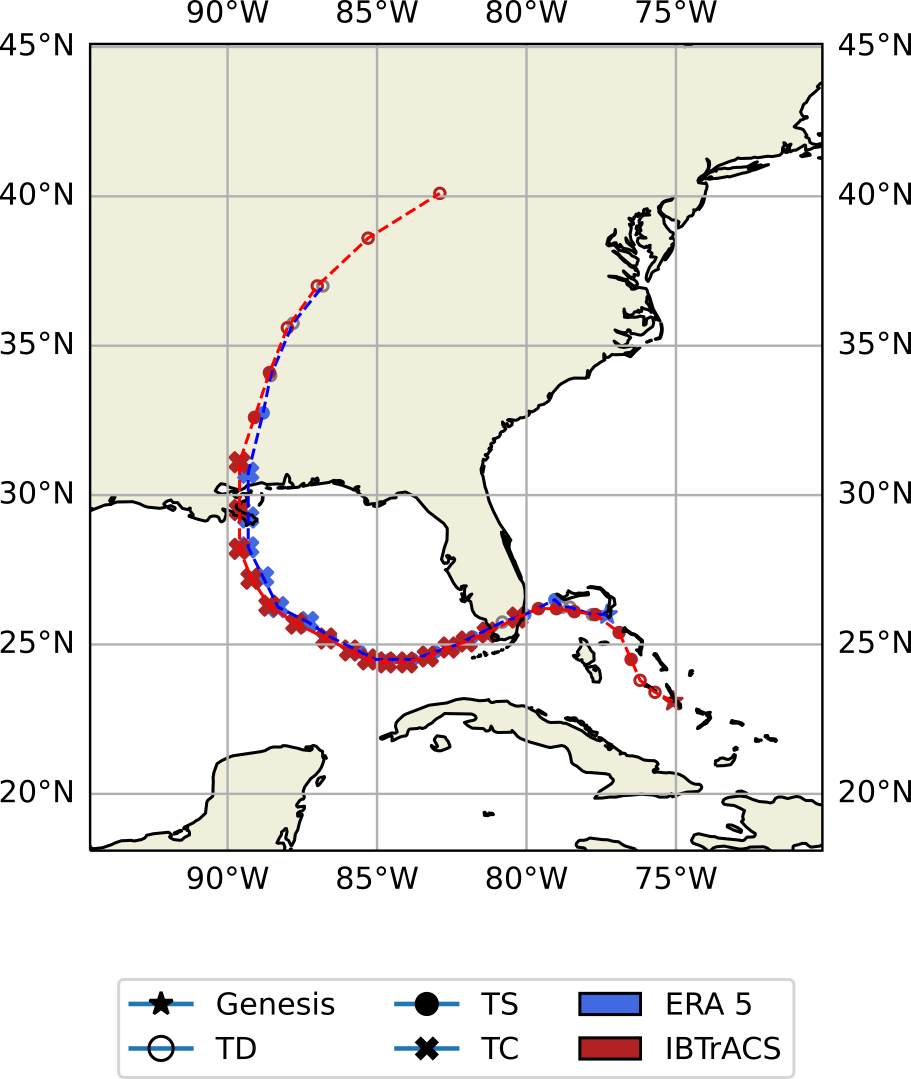
\includegraphics[width=5cm]{Figures/katrina_era5.png}
                    \caption{Ouragan Katrina (2005) observée (rouge) et détectée dans ERA5 (bleu), résultant de l'appariement des trajectoires.}
                \end{figure}
            \end{column}
        }
    \end{columns} 
\end{frame}


%=========================================================
\subsection*{Performances du traqueur}
\begin{frame}[t]
    \frametitle{Performances du traqueur sur ERA5}
    \footnotesize
    \begin{examples}[Probabilité de détection et taux de fausses alertes]    
        \scriptsize
        \[ \text{FAR} = \frac{N_{\text{ERA5}} - N_{\text{Hit}}}{N_{\text{ERA5}}}, \quad\quad \text{POD} = \frac{N_{\text{Hit}}}{N_{\text{IBTrACS}}} \]
        %
        \setlength{\leftmargini}{2.5ex}
        \begin{itemize}
            \item $N_{\text{ERA5}}$ et $N_{\text{IBTrACS}}$ resp. le nombre de trajectoires dans chaque jeu de données
            \item $N_{\text{Hit}}$ le nombre de trajectoires ERA5 appariées à IBTrACS
        \end{itemize}
        $\longrightarrow$ Il suffit \alert{d'une seule échéance} en commun suffit pour compter dans $N_{\text{Hit}}$.
    \end{examples}
    %
    \pause
    %
    \begin{columns}
        \begin{column}{0.56\textwidth}
        \footnotesize
        \vspace{-1.5em}
        \begin{figure}
            \centering
            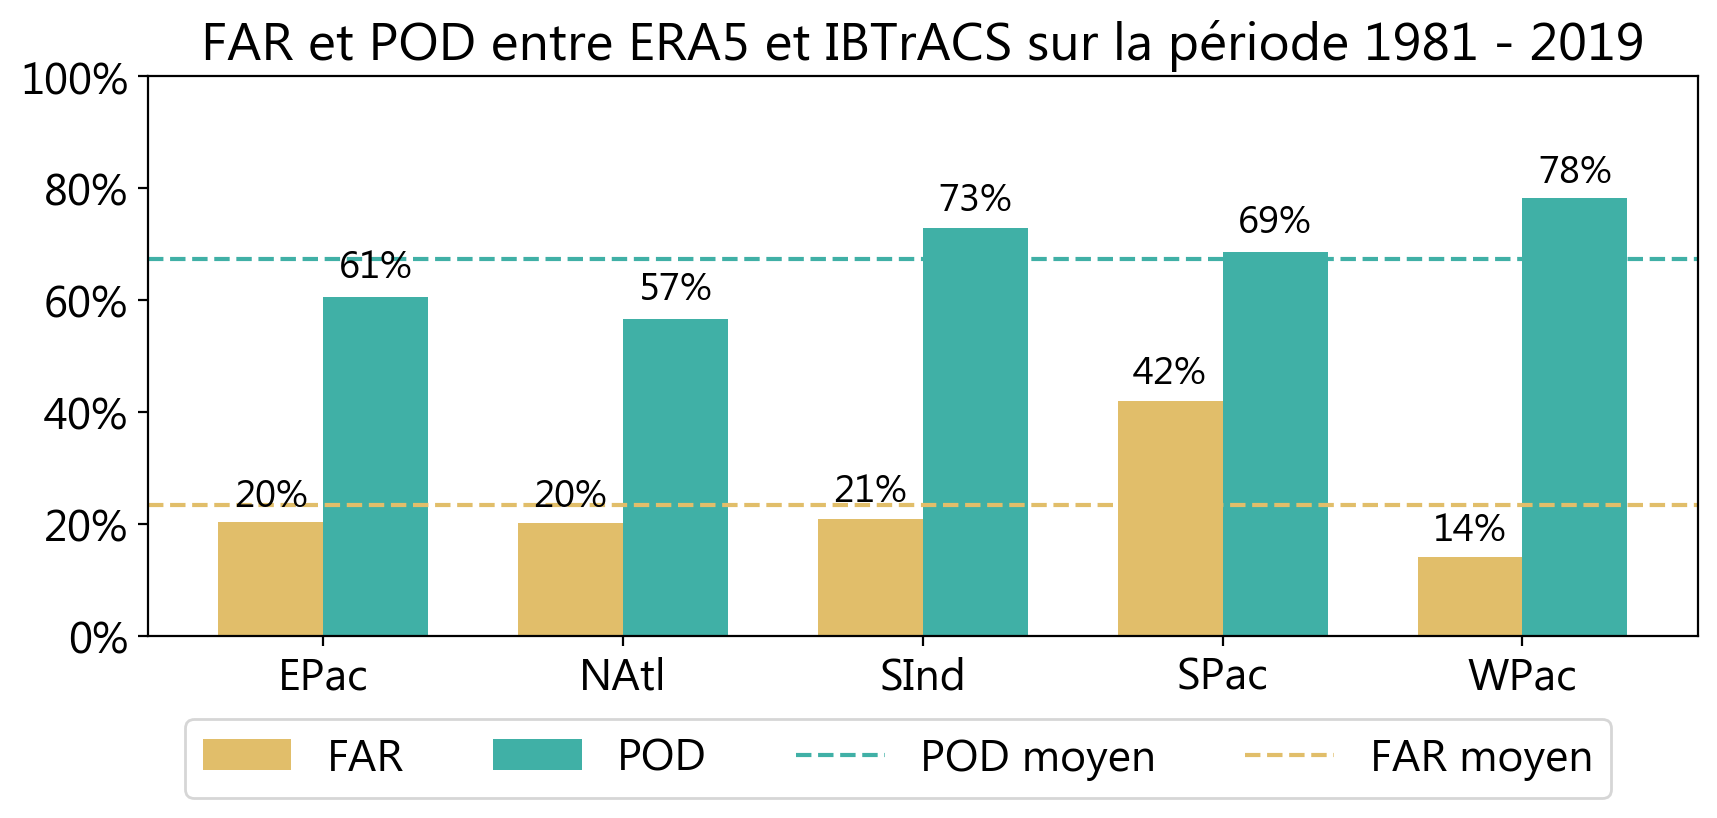
\includegraphics[height=3.8cm]{Figures/far_pod.png}
        \end{figure}
        \end{column}
        \begin{column}{0.36\linewidth}
        \scriptsize
        \vspace{-1em}
        \begin{block}        
            Valeurs seuils optimisées + filtre des systèmes de moyennes latitudes \parencite{hart_cyclone_2003}
            \tcblower
            \setlength{\leftmargini}{2.5ex}
            \alert{Majorité} des systèmes détectés dans ERA5 :
            \begin{itemize}
                \item Moyennes FAR et POD resp. 23,5~\% et 67,4~\%
                \item Performances variables selon les régions
            \end{itemize}
            $\longrightarrow$ Appariement permet d'étudier \underline{uniquement} les \alert{\mbox{systèmes} identifiés} dans IBTrACS
        \end{block}
        \end{column}
    \end{columns}
\end{frame}


%=========================================================
\subsection[Représentation des cyclones dans ERA5]{Représentation des cyclones dans ERA5}
\begin{frame}
    \frametitle{Relation vent-pression dans ERA5}
    \begin{columns}
        \begin{column}{0.5\textwidth}
            \begin{figure}
                \centering
                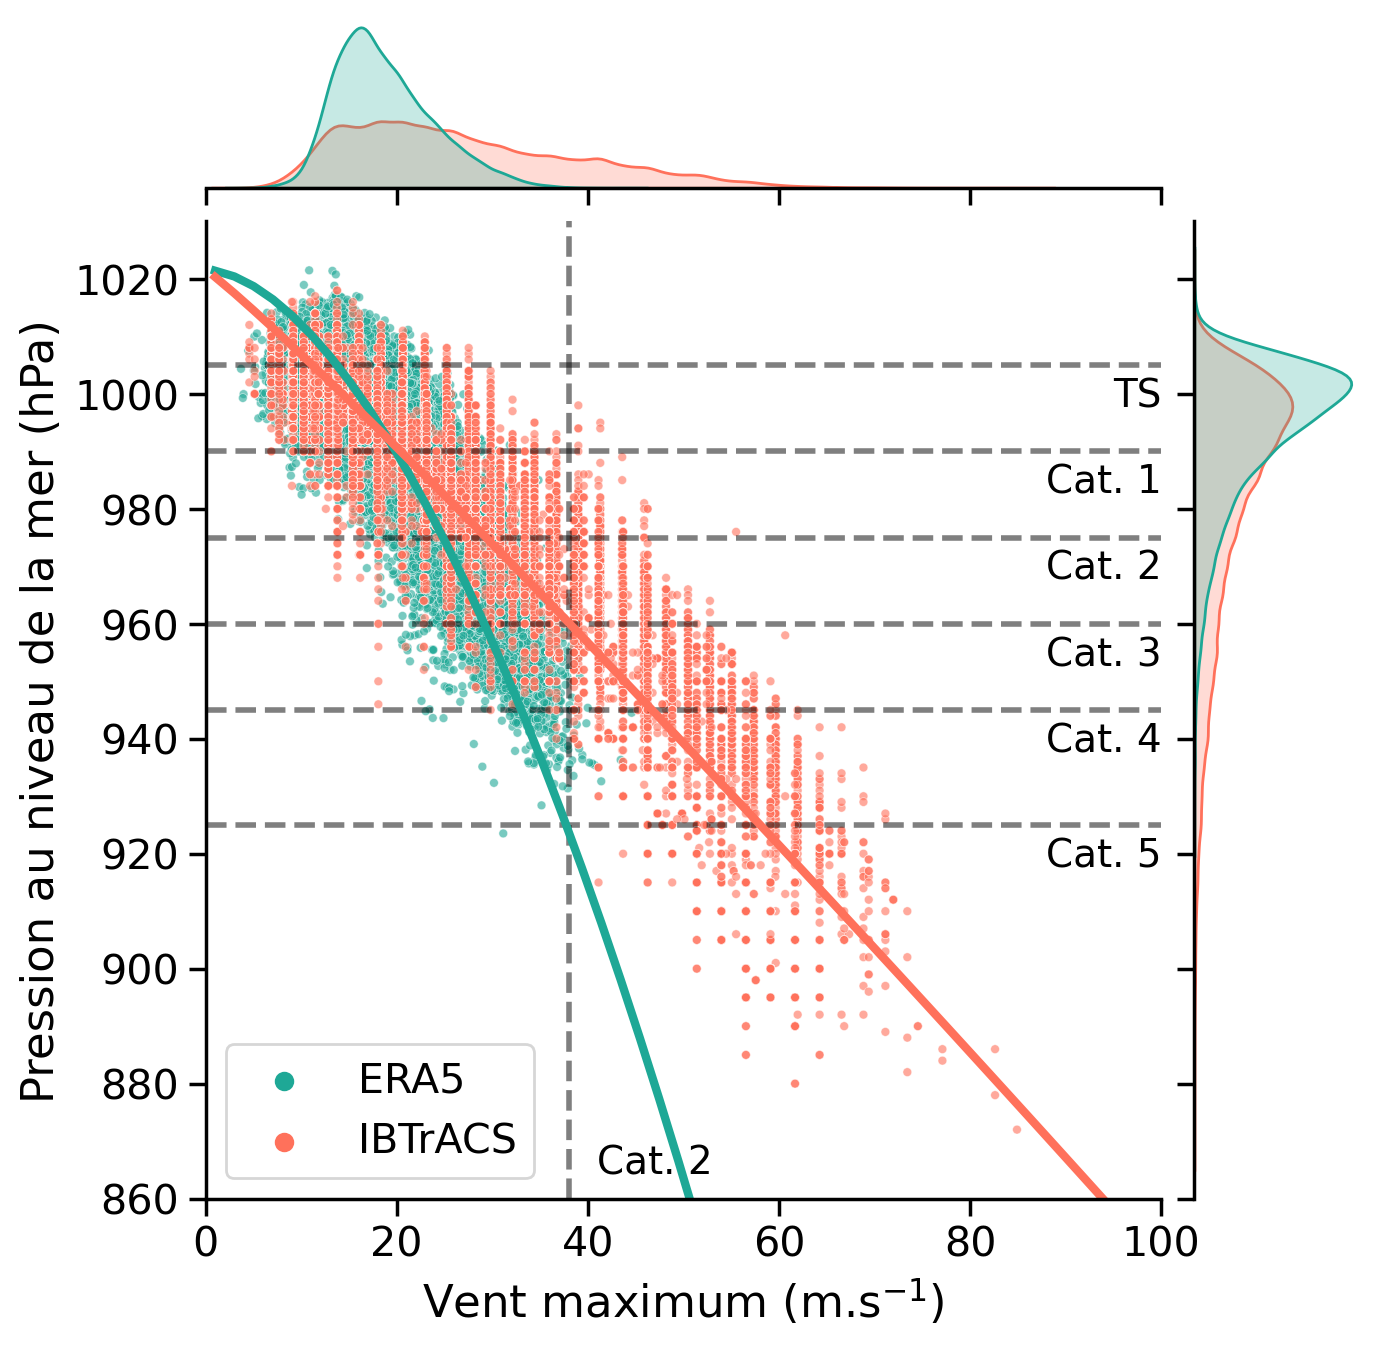
\includegraphics[width=\textwidth]{Figures/ERA5_PV_myVTU.png}
            \end{figure}
        \end{column}
        \begin{column}{0.5\textwidth}
            \footnotesize
            \setlength{\leftmargini}{3.5ex}
            \vspace{1.25ex}
            \begin{examples}[Méthodologie] 
                \begin{itemize}
                    \item Ensemble des échéances partagées pour chaque paire de systèmes\\(58 920 points dans chacun des jeux de données)
                    \item Échelle globale (tous bassins sauf Nord Indien)
                    \item Fit loi de puissance $V = a\Delta P^b$ \parencite{atkinson_tropical_1977}
                \end{itemize}
            \end{examples}
            \vspace{2em}
            \begin{block}
                \begin{itemize}
                    \item \alert{Forte sous-estimation} des vents maximum dans ERA5
                    \item Distribution des minimum de pression \underline{mieux représentée} (Cat 4)
                \end{itemize}
            \end{block}
        \end{column}
    \end{columns} 
\end{frame}

%=========================================================
\begin{frame}
    \frametitle{Classes d'intensité croisées}
    \begin{columns}
        \begin{column}{0.5\textwidth}
            \vspace{1em}
            \begin{figure}
                \centering
                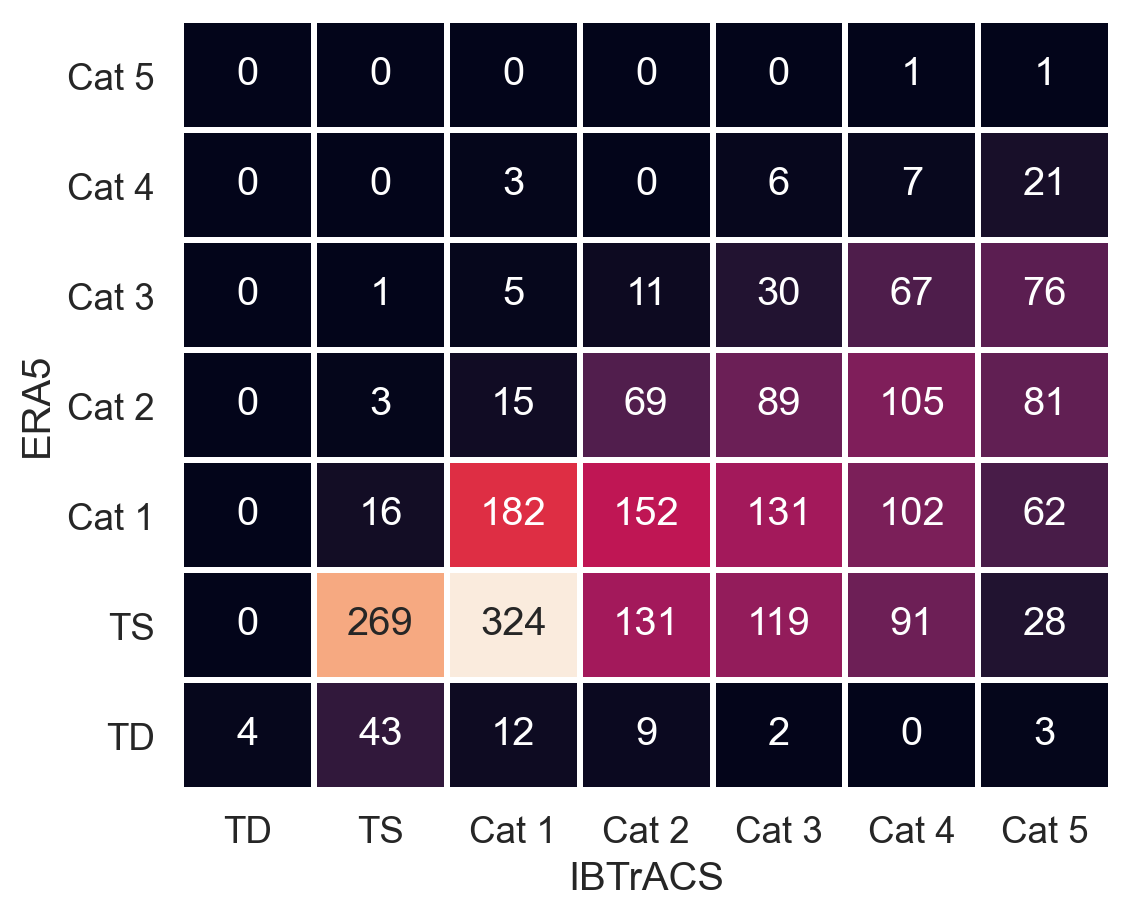
\includegraphics[width=\textwidth]{Figures/crosstable_global_myVTU.png}
            \end{figure}
        \end{column}
        \begin{column}{0.5\textwidth}
            \footnotesize
            \setlength{\leftmargini}{3.5ex}
            \begin{examples}[Méthodologie]
                \begin{itemize}
                    \item Classes Saffir-Simpson basées sur la \alert{pression}\\\parencite{klotzbach_surface_2020}
                    \item Paires de systèmes avec moins de 75\% de valeurs manquantes
                    \item Toutes les régions sauf Nord Indien
                \end{itemize}    
            \end{examples}
            \vspace{2em}
            \begin{block}
               \begin{itemize}
                    \item Accord relatif dans l'ensemble (pente attendue)
                    \item \alert{Dispersion importante} vers les catégories les plus hautes
               \end{itemize} 
            \end{block}
        \end{column}
    \end{columns} 
\end{frame}

%=========================================================
\begin{frame}[t]
    \frametitle{Décalage dans les maximum d'intensité}
    \begin{figure}
        \centering
        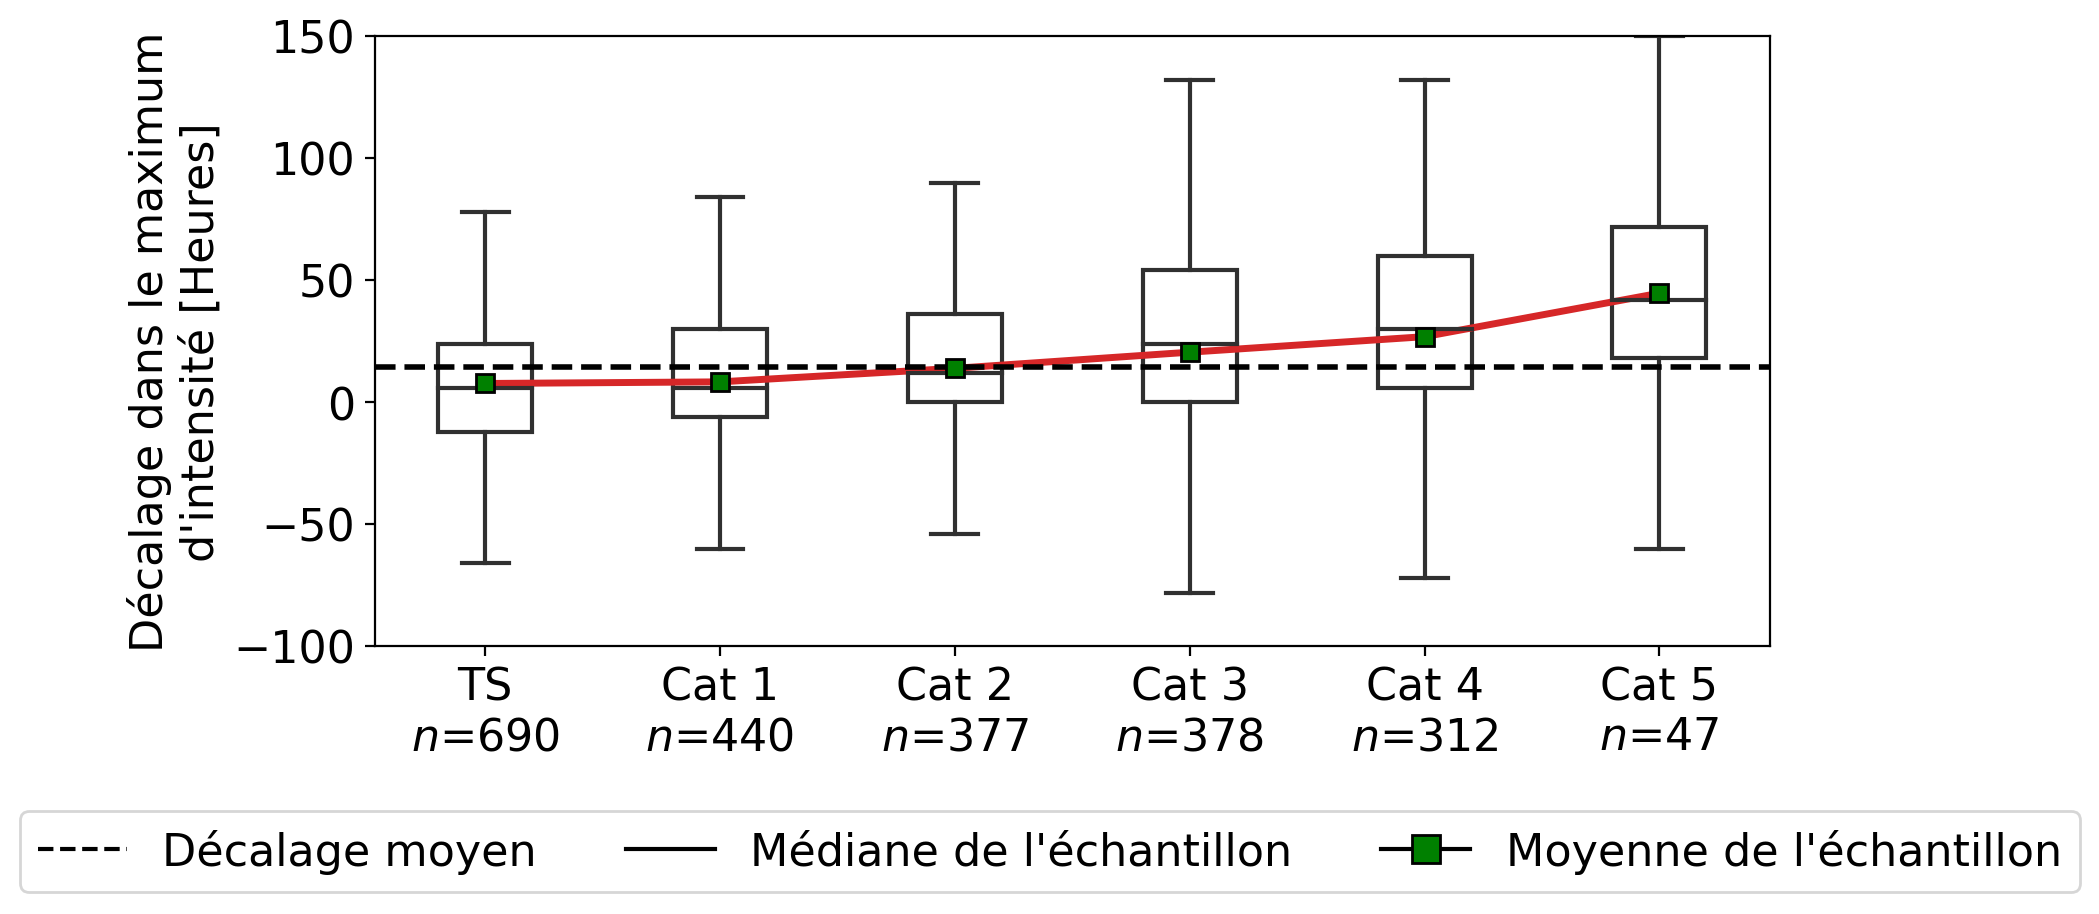
\includegraphics[width=0.8\textwidth]{Figures/lag_max_intensity_myVTU.png}
    \end{figure}
    \begin{columns}
        \footnotesize
        \setlength{\leftmargini}{3ex}
        \begin{column}{0.5\textwidth}
            \begin{examples}
                \begin{itemize}
                    \item Délais (en heures) entre le maximum d'intensité des paires ERA5/IBTrACS par classe d'intensité (IBTrACS)
                    \item Délai > 0 indique que le TC dans ERA5 est \underline{en retard}
                \end{itemize}
            \end{examples}
        \end{column}
        \begin{column}{0.5\textwidth}
            \begin{block} 
                \begin{itemize}
                    \item Délai moyen toutes catégories de \alert{+13 heures} (significatif)
                    \item Délai \alert{augmente} avec la classe d'intensité\\(45 heures pour Cat 5)
                \end{itemize}
            \end{block}
        \end{column}
    \end{columns}
\end{frame}


%=========================================================
\begin{frame}[c]
    \frametitle{Représentation des cyclones dans ERA5}
    \framesubtitle{Conclusion}
    %Slide de conclusion sur cette partie : Pourquoi ces résultats sont importants :
    %\begin{itemize}
    %    \item Attention quand on veut aller voir la tête d'un TC observé dans ERA5 (vent sous-estimé + pas forcément même classe d'intensité)
    %    \item C'est également fortement déconseillé d'aller directement extraire les champs ERA5 en lieu et place du max d'intensité d'un TC observé (à cause du
    %        délai)
    %\end{itemize}
    \begin{block}[Messages clefs \parencite{dulac_assessing_2023}]
        \small
        \begin{enumerate}
            \setlength\itemsep{1em}
            \item<1-> \alert{Bonnes performances} du traqueur (FAR et POD), grâce à l'optimisation et à l'utilisation d'un filtre de systèmes de
                moyennes latitudes adapté
            \item<2-> Forte \alert{sous-estimation} des vents associés aux TC, pression minimale mieux représentée
            \item<3-> \alert{Dipersion} dans les classes d'intensité entre ERA5 et IBTrACS + \alert{retard} dans l'intensification
        \end{enumerate}
        \vspace{1em}
        \onslide<4->{\hskip1em $\longrightarrow$ Nécessité de traquer ERA5 pour l'étude des TC}
    \end{block}
    \onslide<5->{
        \large 
        \vspace{\baselineskip}
        \begin{center}
            Vers des métriques d'évaluation de la \alert{qualité} des trajectoires ?
        \end{center}
    }
\end{frame}

%=========================================================
\subsection[Similarité des trajectoires]{Métriques de similarité des trajectoires}
\makesubsecslide
\begin{frame}[c]
    \frametitle{Similarité des trajectoires}
    \framesubtitle{Motivations}
    \small
    \vspace{1em}
    \begin{definition}
        \begin{itemize}
            \item Métriques de performances du traqueur \alert{intégrée} sur les trajectoires (par rapport au FAR et POD)
            %\item Proportion non-nulle des composantes ERA5 de chaque paire de trajectoires qui se trouve à plus de \mbox{300 km} de la composante IBTrACS
            \item Appariement $<$ 100~\% : Trajectoires détectées trop courtes \alert{et/ou} située à plus de 300 km d'IBTrACS
        \end{itemize}
    \end{definition}
    %\vspace{1em}
    \begin{figure}
        \centering
        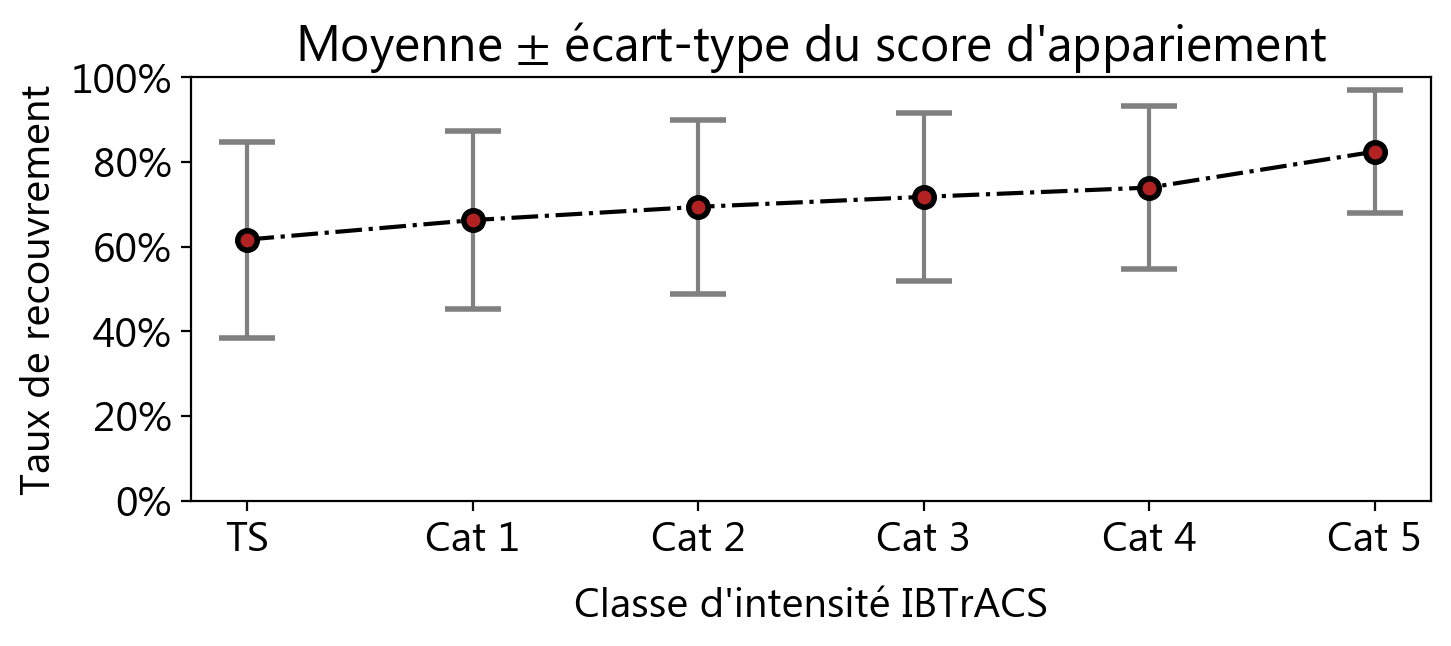
\includegraphics[height=4cm]{Figures/coverage_ratio.png}
        \captionsetup{width=0.75\textwidth}
        \caption{Statistiques réalisées sur les 2 244 paires de trajectoires de \cite{dulac_assessing_2023} dont l'intensité de la composante IBTrACS est
        classifiable (moins de 75\% de valeurs manquantes) et sur les 5 bassins géographiques (NInd exclu).}
    \end{figure}
\end{frame}

%=========================================================
\begin{frame}[c]
    \frametitle{Similarité des trajectoires}
    \framesubtitle{Principe de fonctionnement}
    \begin{columns}[t]
        \begin{column}{0.4\textwidth}
           \onslide<1->{ 
               \vspace{-1em}
               \footnotesize
               \begin{definition}
                   \scriptsize
                   \centering
                   Décomposition d'une trajectoire en séquence de vecteurs de déplacement relatifs
               \end{definition}
           }
           %
           \onslide<4->{
               \footnotesize
               \begin{examples}[Similarité angulaire $S_\theta$]
                   \scriptsize
                   Pour deux vecteurs au temps $t$ issus de deux trajectoires différentes :
                   %
                   \onslide<5->{
                       \setlength{\belowdisplayskip}{-2mm}
                       \begin{align*}
                           \cos \theta &= \frac{\mathbf{c}_i \cdot \mathbf{q}_i}{\lVert \mathbf{c}_i \rVert \lVert \mathbf{q}_i \rVert} \in [-1; 1] \\
                           S_{\theta} &= 1 - \frac{\theta}{\pi} \in [0; 1]
                       \end{align*}
                   }
               \end{examples}
           }
           %
           \onslide<6->{
           \footnotesize
           \begin{block}
               \scriptsize
               \setlength{\leftmargini}{2.5ex}
               \begin{itemize}
                   \item<6-> \alert{Intersection} $C \cap Q$ : Points où les deux trajectoires co-existent aux mêmes temps $t$
                   \item<7-> \textcolor{green}{Différence symmétrique} $C \ominus Q$ : Points où une seule trajectoire est définie
                   \item<8-> Union $C \cup Q$ : Ensemble des points des deux trajectoires
               \end{itemize}
           \end{block}
       }
        \end{column}
        \begin{column}{0.6\textwidth}
            \vspace{-3.5em}
            \begin{figure}
                \centering
                \includegraphics<1>[width=\textwidth]{Figures/schema_vec_sequence/step0.png}%
                \includegraphics<2>[width=\textwidth]{Figures/schema_vec_sequence/step1.png}%
                \includegraphics<3>[width=\textwidth]{Figures/schema_vec_sequence/step2.png}%
                \includegraphics<4>[width=\textwidth]{Figures/schema_vec_sequence/step3.png}%
                \includegraphics<5>[width=\textwidth]{Figures/schema_vec_sequence/step4.png}%
                \includegraphics<6->[width=\textwidth]{Figures/schema_vec_sequence/step5.png}%
            \end{figure} 
        \end{column}
    \end{columns} 
\end{frame}

%=========================================================
\begin{frame}[t]
    \frametitle{Métriques de similarité}
    %\vskip0ptplus1filll\relax
    \begin{columns}[t]
        \begin{column}{0.66\textwidth}
            \footnotesize
            \vspace{-1.5em}
            \begin{examples}[Métriques de similarité angulaire moyenne ({MAS, \textit{Mean Angular Similarity}})]
                \begin{enumerate}[(a)]
                    \item<1-> $\text{MAS}^\cap = \bar{S_\theta}^\cap = \frac{1}{\alert{N_\cap}} \sum_{i=1}^{N_\cap} S_\theta (\mathbf{c}_i, \mathbf{q}_i)$
                    \item<2-> $\text{MAS}^\cup = \bar{S_\theta}^\cup = \frac{1}{\underbrace{\textcolor{blue}{N_\cap} + \textcolor{red}{N_\ominus}}_{=
                        N_\cup}} \sum_{i=1}^{N_\cap} S_\theta (\mathbf{c}_i, \mathbf{q}_i)$
                    \item<3-> $\text{wMAS} = \frac{ \alert{w_1}}{ \alert{w_1 N_\cap} + \textcolor{red}{w_2 N_\ominus}} \sum_{i=1}^{N_\cap} S_{\theta}(\mathbf{c}_i, \mathbf{q}_i) \quad\quad 
                    \begin{cases}
                        \alert{w_1} = 1 + \bar{S_\theta}^\cap \\
                        \textcolor{red}{w_2} = 2 - \bar{S_\theta}^\cap \\
                    \end{cases}$
                \end{enumerate}
            \end{examples}
        \end{column}
        \begin{column}{0.33\textwidth}
            \footnotesize
            \onslide<4->{
                \vspace{-7em}
                \begin{figure}
                    \centering
                    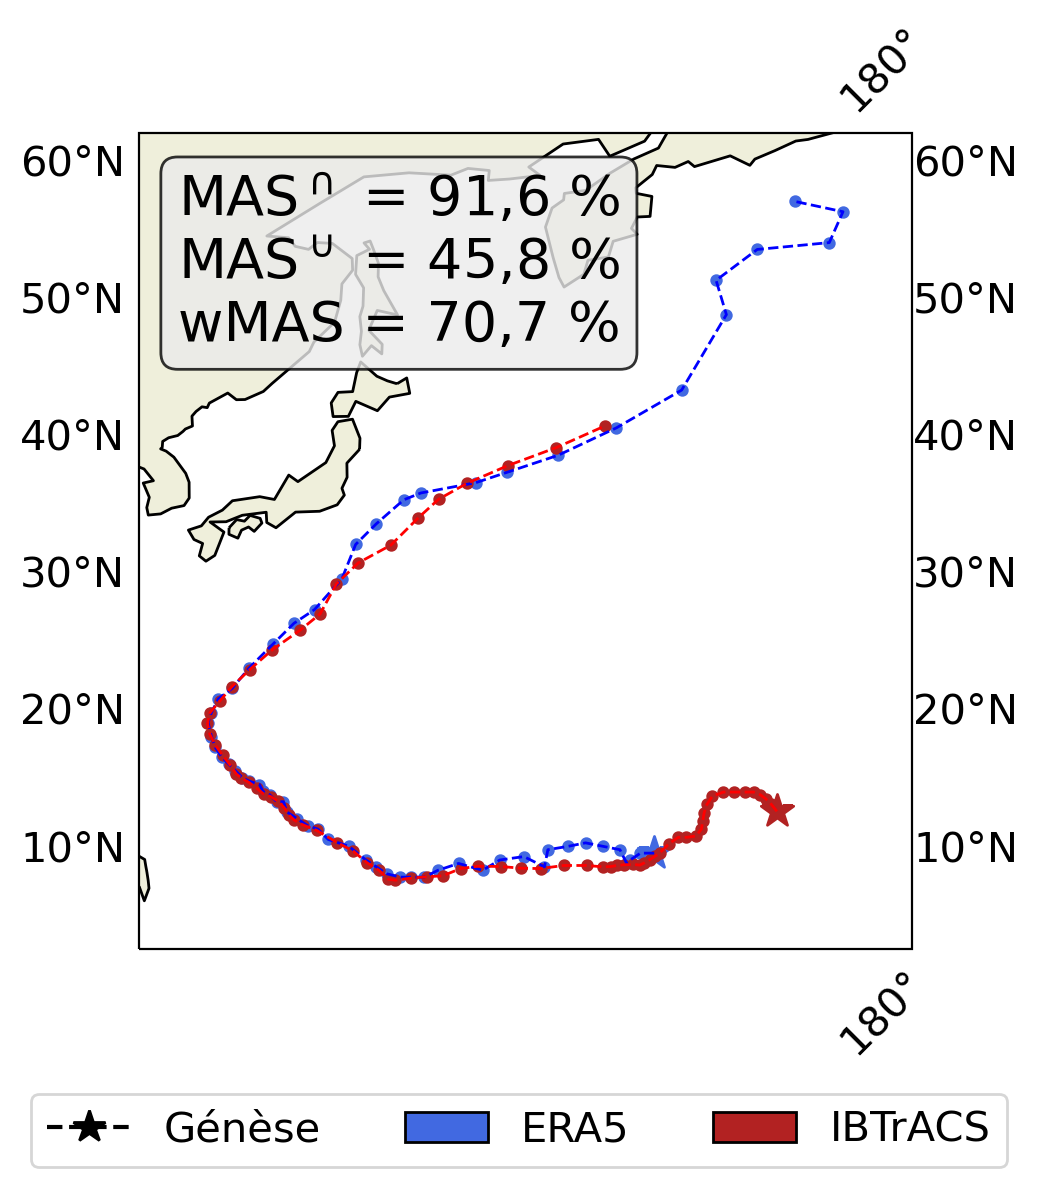
\includegraphics[width=0.9\textwidth]{Figures/exemple_similarity.png}
                \end{figure}
            }
        \end{column}
    \end{columns}
    \onslide<5->{
        \vspace{-0.5em}
        \begin{figure}
            \centering
            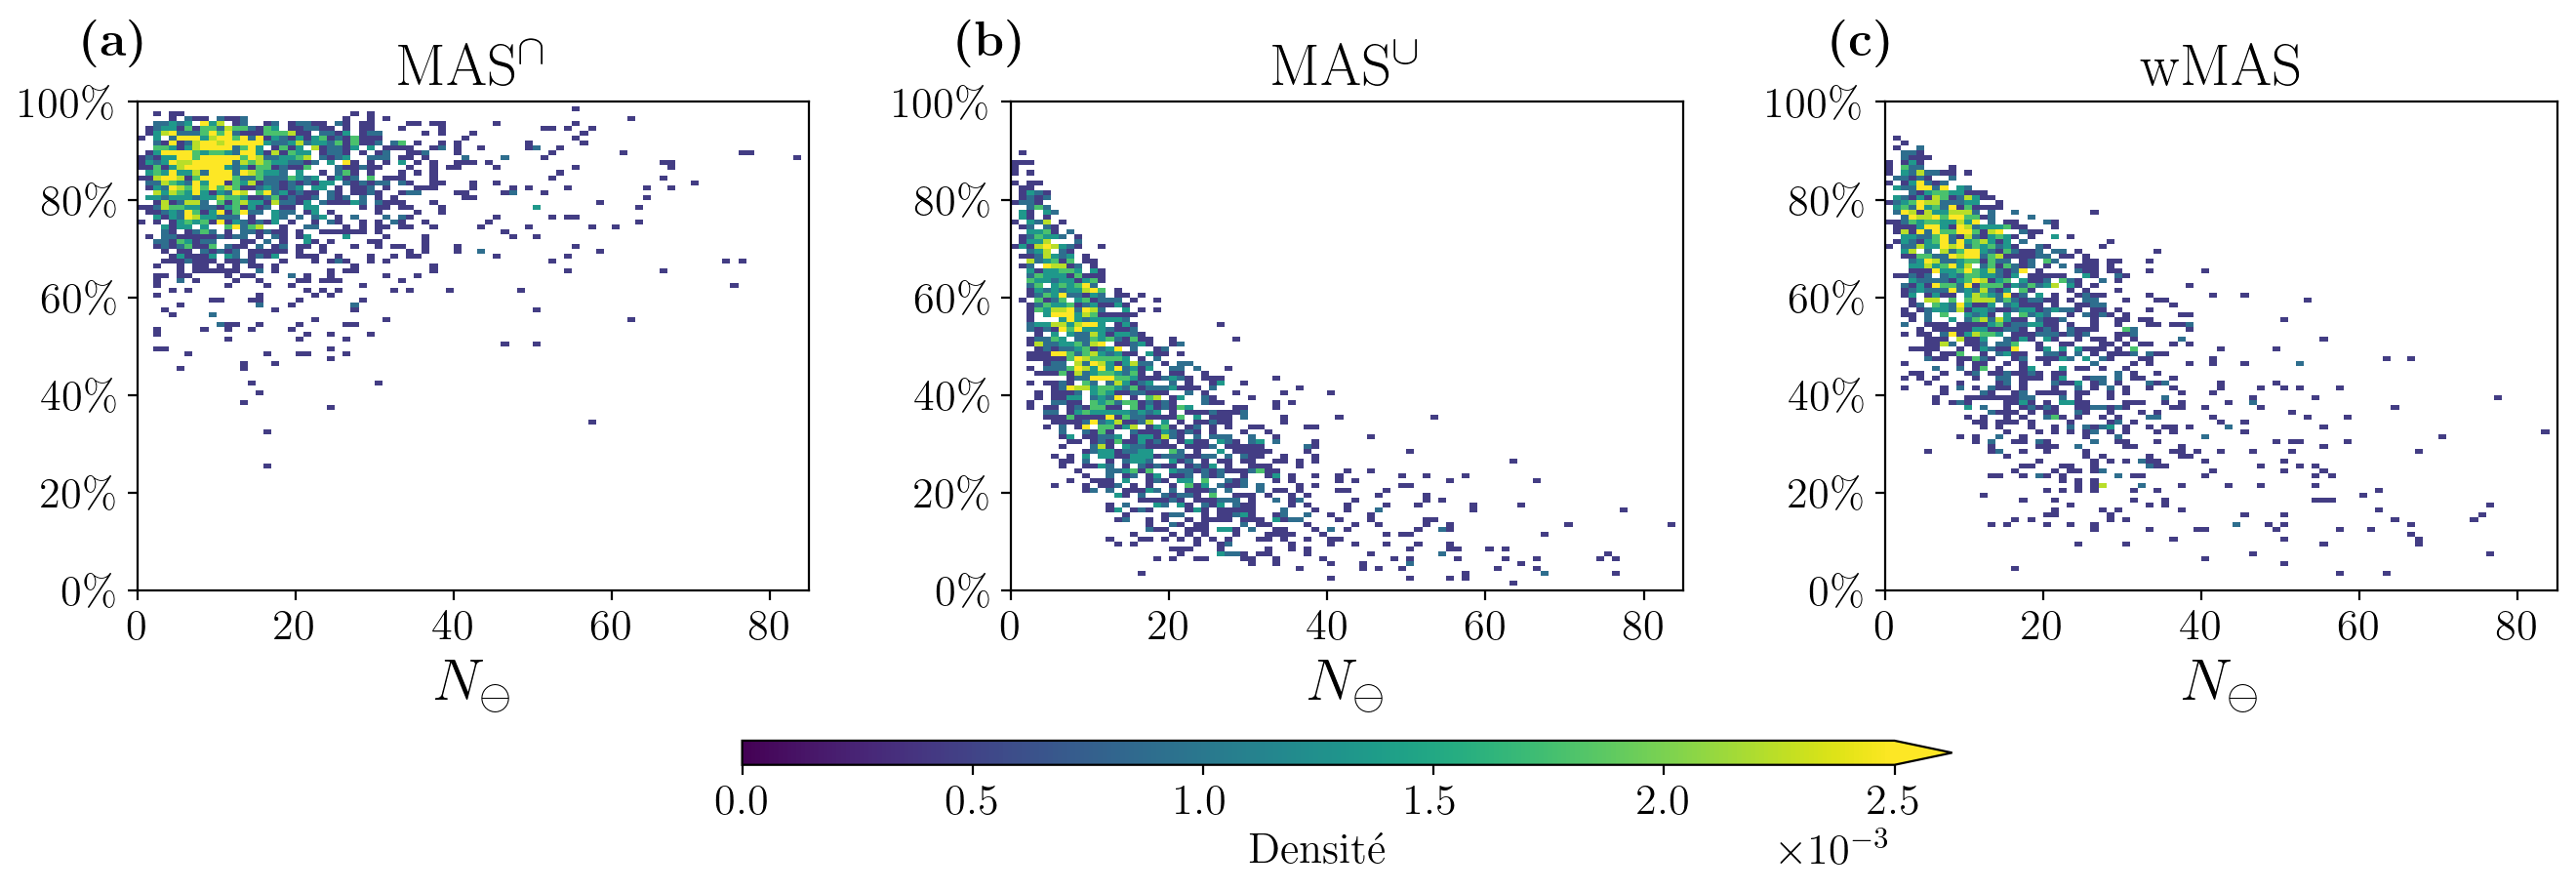
\includegraphics[height=3.5cm]{Figures/MAS_vs_Ndiff.png}
        \end{figure}
    }
\end{frame}

%=========================================================
\begin{frame}[c]
    \frametitle{Application des métriques}
    \framesubtitle{Optimisation des paramètres du traqueur : Quel impact ?}
    %Introduire la situation (possiblement avec un schéma pour clarifier le plus possible) :
    %\begin{itemize}
    %    \item Deux jeux de trajectoires ERA5 à différents paramètres seuils (lister les paramètres)
    %    \item Les deux jeux sont appariés à IBTrACS : 2 trajectoires ERA5 pour chaque trajectoire IBTrACS
    %    \item $\longrightarrow$ On regarde le changement de similarité entre les deux paires
    %\end{itemize}
    \begin{columns}
        \begin{column}{0.6\textwidth}
           \footnotesize
           \begin{definition}
               \centering
               Calcul de la différence de similarité dans les paires ERA5 / IBTrACS avant et après l'optimisation des paramètres
           \end{definition}
           \vspace{1em}
           \begin{block}[Jeux de trajectoires]
               1 649 \alert{triplets} de trajectoires :
               \begin{itemize}
                    \item IBTrACS v4
                    \item Trajectoires ERA5 utilisées dans \cite{dulac_assessing_2023} (Optimisées)
                    \item Trajectoires ERA5 \alert{avant} optimisation des paramètres :
                        \begin{itemize}
                            \footnotesize
                            \item \textbf{VOR} = 5$\cdot$10$^{\text{-5}}$ s$^{\text{-1}}$ (resp. 15$\cdot$10$^{\text{-5}}$ s$^{\text{-1}}$)
                            \item \textbf{RES} = 15 m.s$^{\text{-1}}$ (resp. 5m~.s$^{\text{-1}}$)
                            \item \textbf{PT} = -2~K (resp. -1~K)
                            \item Paramètre de relaxation \alert{identique} (25$\cdot$10$^{\text{-5}}$ s$^{\text{-1}}$)
                        \end{itemize}
               \end{itemize}
               $\longrightarrow$ \alert{Deux trajectoires} ERA5 pour chaque trajectoire IBTrACS
           \end{block}
        \end{column}
        \begin{column}{0.4\textwidth}
            \vspace{-2em} 
            \begin{figure}
                \centering
                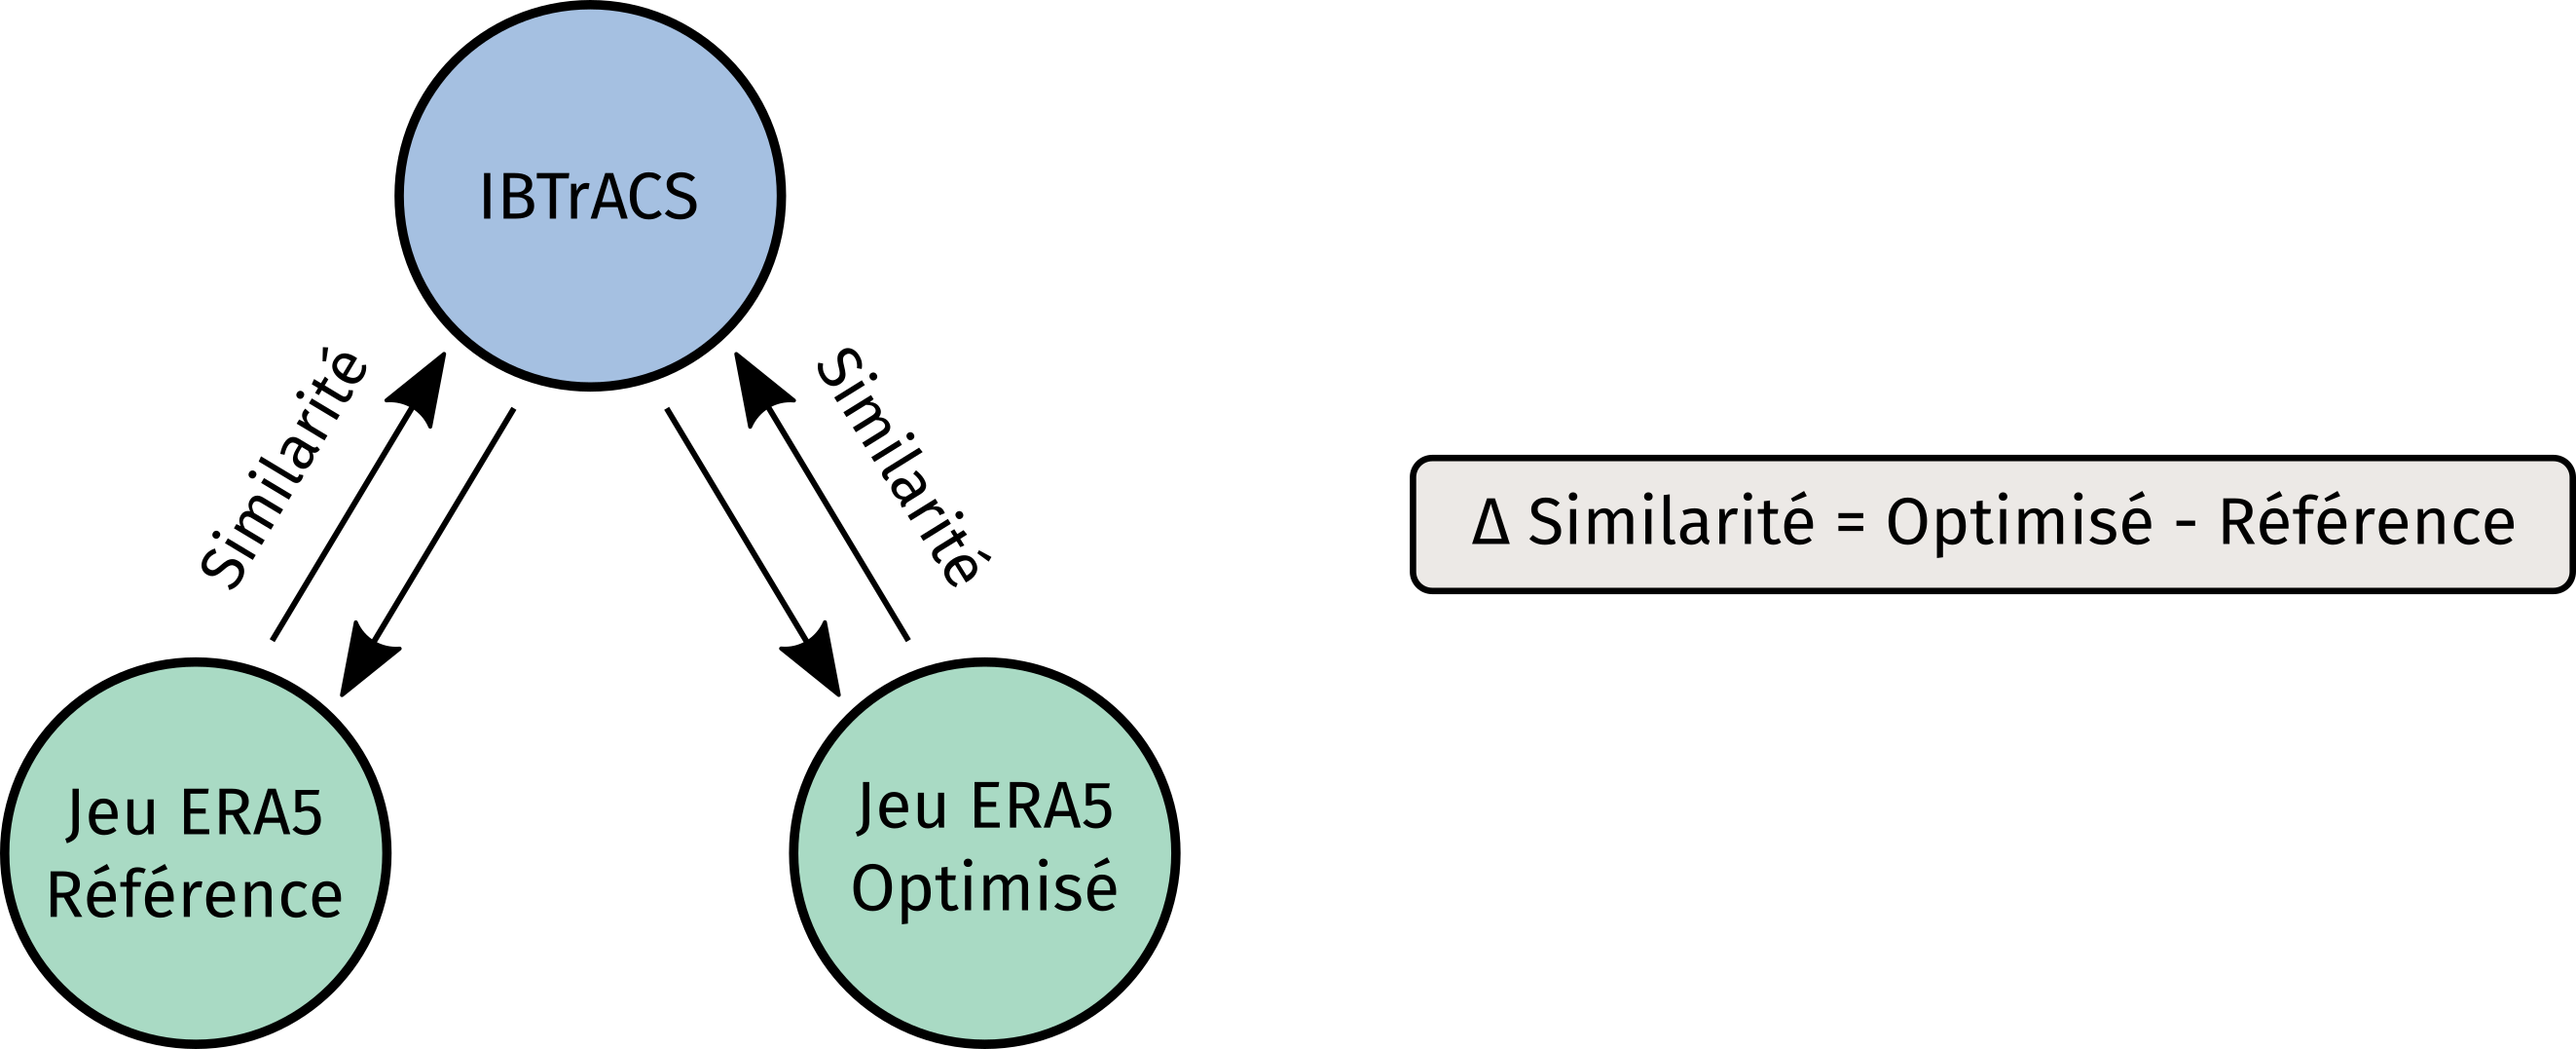
\includegraphics[width=\textwidth]{Figures/schema_application_similarite.png}
            \end{figure} 
        \end{column}
    \end{columns}
\end{frame}

%=========================================================
\begin{frame}[c]
    \frametitle{Changements dans les similarités}
    \framesubtitle{Résultats}
    \begin{columns}
        \begin{column}{0.7\textwidth}
            \begin{center}
                \includegraphics<1>[width=\textwidth]{Figures/delta_MAS_hists_only.png}%
                %\includegraphics<2>[width=\textwidth]{Figures/delta_MAS.png}%
                \includegraphics<2->[width=\textwidth]{Figures/delta_MAS_fit.png}%
            \end{center}
        \end{column}
        \begin{column}{0.3\textwidth}
            \footnotesize
            \onslide<2->{
                \begin{block}
                    $\overline{\Delta N_\ominus} =$ -0,8 échéances\\
                    \vspace{\baselineskip}
                    $\longrightarrow$ Amélioration de la similarité par \alert{réduction} da la différence de temporalité
                \end{block}
            }
            %
            \onslide<3->{
                \vspace{1em}
                \begin{alertblock}[Lorsque {$\Delta N_\ominus = 0$} \underline{et} {$\Delta N_\cap = 0$}]
                    À temporalité \alert{inchangée} ($n =$ 691) :
                    \begin{enumerate}[(a)]
                        \item $\overline{\Delta \text{MAS}^\cap} =$ +0,57 p.p
                        \item $\overline{\Delta \text{MAS}^\cup} =$ +0,34 p.p
                        \item $\overline{\Delta \text{wMAS}} =$ +0,54 p.p
                    \end{enumerate}
                \end{alertblock}
            }
        \end{column}
    \end{columns}
\end{frame}

%=========================================================
\begin{frame}
    \frametitle{Détection et suivi des TC dans ERA5}
    \framesubtitle{Synthèse}
    \begin{block}[Messages clefs]
        \small
        \begin{enumerate}
            \setlength\itemsep{1em}
            \item<1-> Utilisation de la réanalyse ERA5 pour caractériser le schéma de détection du CNRM
            \item<2-> Appariement des trajectoires détectées avec les trajectoires observées
            \item<3-> Métrique FAR et POD : Détection binaire
            \item<4-> Métrique de similarité des trajectoires : Combine une information sur la position et sur la durée
        \end{enumerate}
    \end{block}
\end{frame}

%=========================================================
\section[Indices de cyclogénèse]{Indices de cyclogénèse : Vers une meilleure représentation de la variabilité interannuelle}
\begin{frame}[c]
    \frametitle{Plan}
    \addtocounter{framesinsection}{-1}
    \tableofcontents[currentsection,hideallsubsections,sections={1-3}]
    \vspace{-3em}
    \tableofcontents[hideallsubsections,sections={4-}]
\end{frame}
%
\begin{frame}[c]
    \frametitle{Plan}
    \addtocounter{framesinsection}{-1}
    \tableofcontents[currentsection,hideothersubsections]
\end{frame}

\makesecslide

%=========================================================
\subsection*{Motivations}
\begin{frame}[t]
    \frametitle{Introduction}
    \framesubtitle{Les indices de cyclogénèse}
    \small
    \begin{definition}[Définition]
        Relation mathématique reliant la fréquence d'occurrence des TC (cyclogénèses) avec l'environnement de grande échelle.
        \begin{align*}
            N_{\text{TC}} &= \iint\limits_{D} \underbrace{\rho(\phi, \lambda)}_{\text{Indice}} \; d\phi \, d\lambda \\
            \rho &= \underbrace{\vphantom{X_{\text{Dyn}}}\textcolor{green}{A}}_{\textcolor{green}{\text{Calibration}}} \times
            \underbrace{\vphantom{X_{\text{Dyn}}}\textcolor{red}{X_{\text{Th}}}}_{\textcolor{red}{\text{Thermique}}} \times
            \underbrace{\textcolor{violet}{X_{\text{Dyn}}}}_{\textcolor{violet}{\text{Dynamique}}}
        \end{align*}
        Composés d'une composante \textcolor{red}{thermique}, d'une composante \textcolor{violet}{dynamique} et sont \textcolor{green}{calibrés} pour simuler la
        quantité moyenne souhaitée 
    \end{definition}
    \vspace{1.5em}
    \uncover<2->{
        \begin{alertblock}
            \centering
            Les indices sont initialement conçus pour reproduire la climatologie spatiale et saisonnière de l'activité cyclonique
        \end{alertblock}
    }
\end{frame}

%=========================================================
\begin{frame}
    \frametitle{Introduction}
    \onslide<1->{
        \begin{columns}
                \begin{column}{0.5\textwidth}
                    \vspace{-2em}
                    \begin{figure}
                        \centering
                        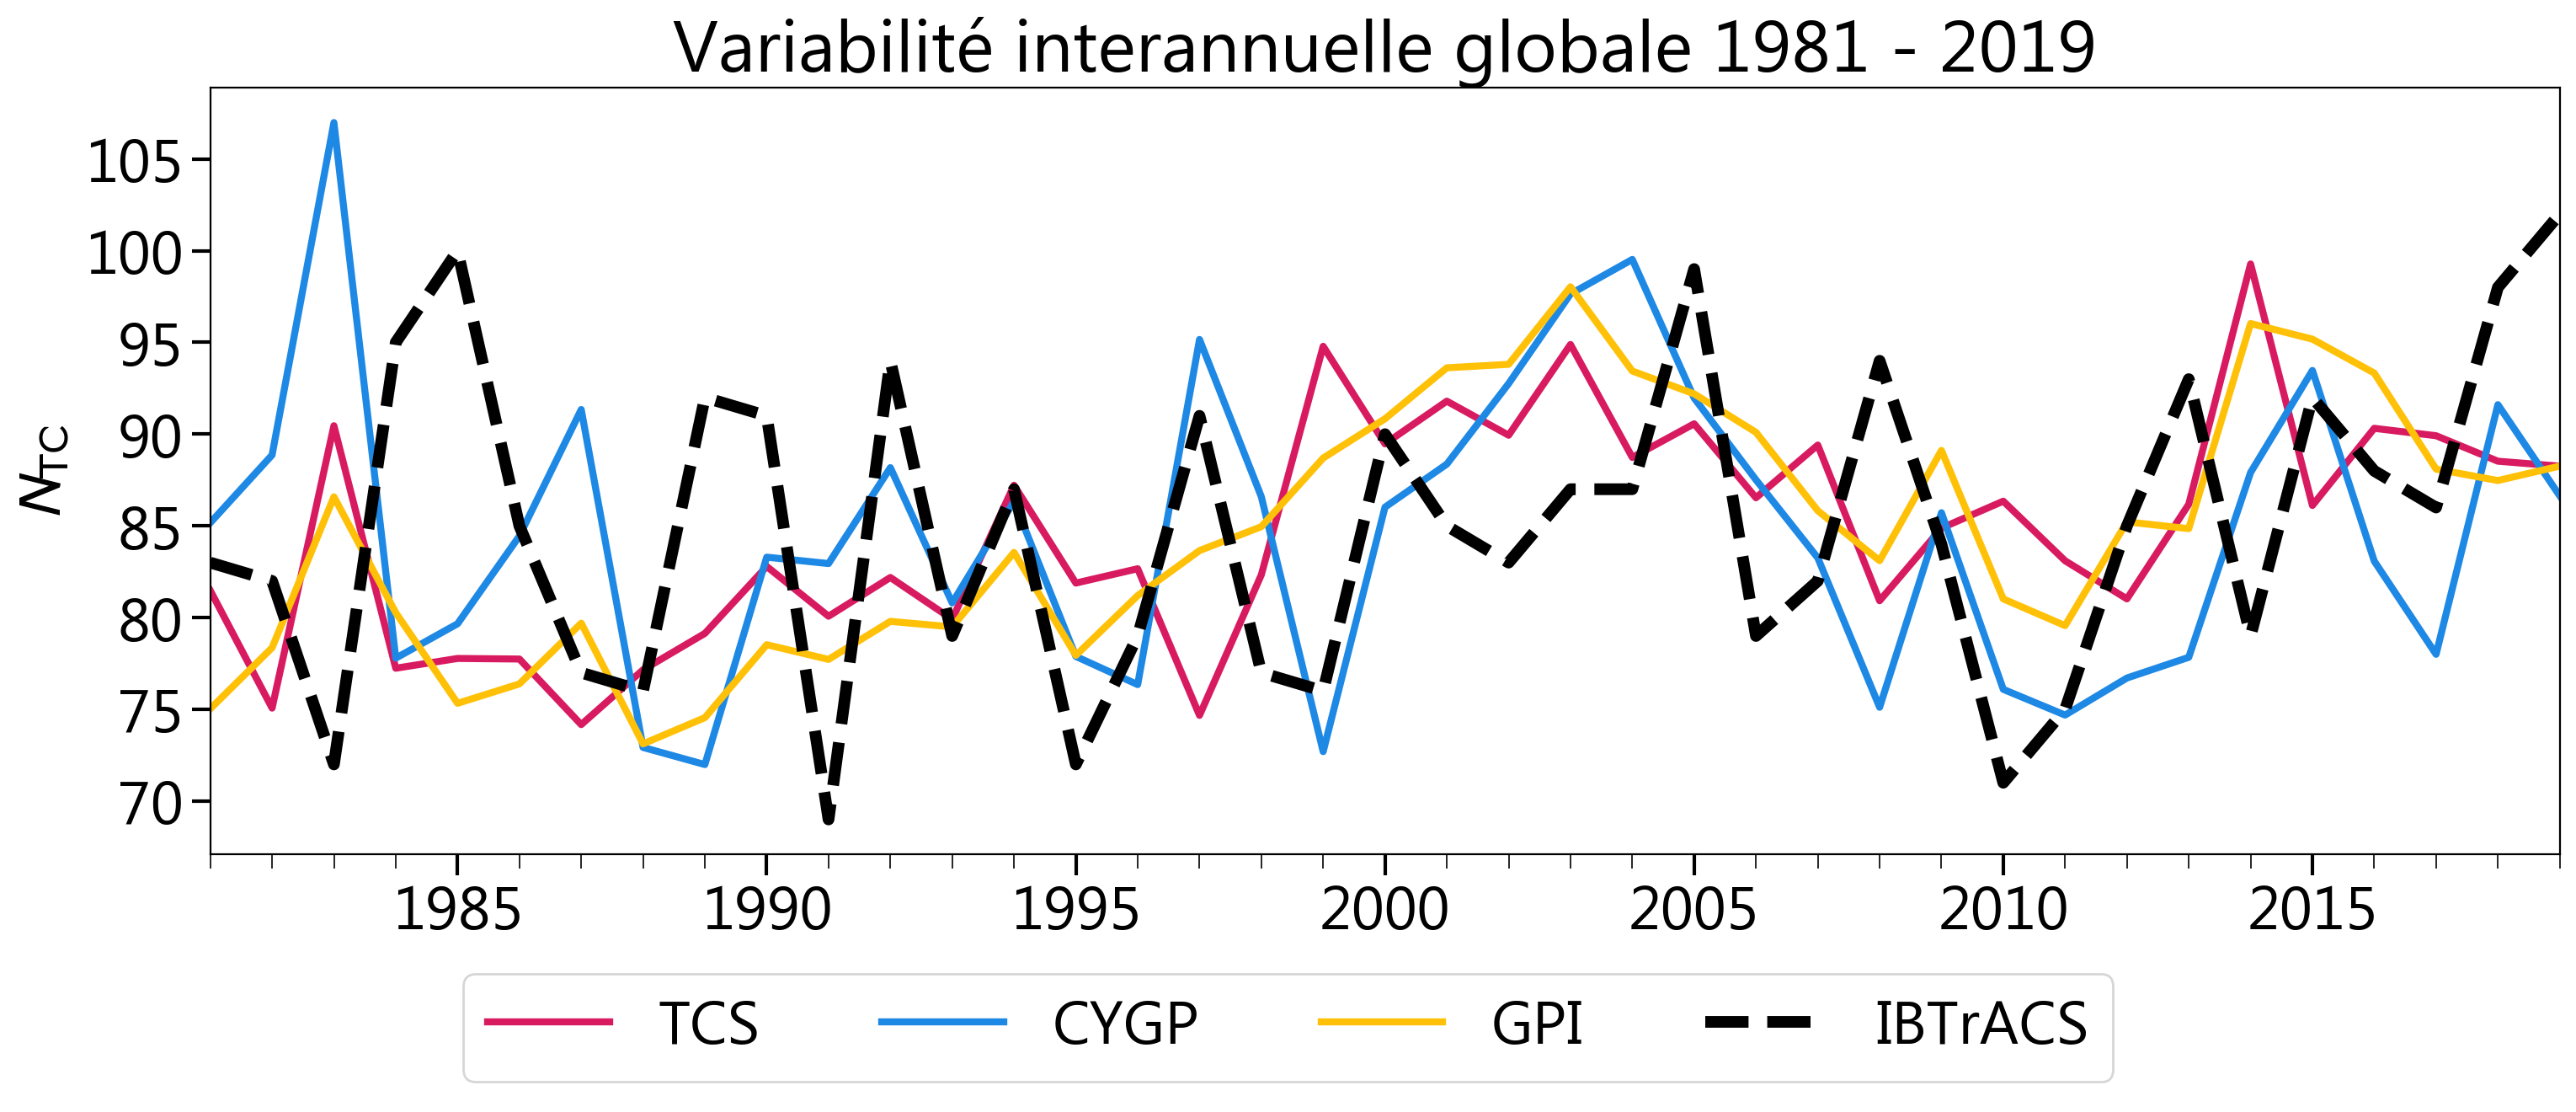
\includegraphics[height=3.2cm]{Figures/tcs_cygp_gpi_interannual.png} 
                    \end{figure}
                \end{column}
                \begin{column}{0.5\textwidth}
                   \scriptsize
                   \vspace{-3.5em}
                   \begin{table}[h]
                       \centering
                       \caption{\footnotesize Corrélation de la variabilité\\ interannuelle ERA5 avec IBTrACS}
                       \begin{tabular}{l|c|c|c}
                           & TCS & CYGP & GPI \\
                           \hline
                           Ouest Pac. & 0,03 & 0,46 & 0,06 \\
                           Est Pac. & 0,7 & 0,62 & 0,64 \\
                           Nord Atl. & 0,71 & 0,7 & 0,79 \\
                           Sud Pac. & 0,35 & 0,57 & 0,39 \\
                           S.O Ind. & 0,21 & 0,37 & 0,27 \\
                           S.E Ind. & 0,22 & 0,16 & 0,12 \\
                       \end{tabular}
                   \end{table}
                \end{column}
        \end{columns}
    }
    %
    \footnotesize
    \onslide<2->{
        \begin{block}[Indice de Tippett{,} ou TCS \parencite{tippett_poisson_2011}]
            \begin{equation*}
                \text{TCS} = \exp \Big( b_0 + \underbrace{\textcolor{violet}{b_\eta \eta + b_{V_{\text{shear}}} V_{\text{shear}}}}_{\text{Dynamique}} +
                \underbrace{\vphantom{b_\eta \eta + b_{V_{\text{shear}}} V_{\text{shear}}} \textcolor{red}{b_H H + b_T T}}_{\text{Thermique}} + \log \cos \phi \Big)
                \qquad \scriptsize\text{[TC par unité de surface et par unité de temps]}
            \end{equation*}
            %
            \scriptsize
            Avec:
            \vspace{-1em}
            \begin{columns}[t]
                \begin{column}{0.5\textwidth}
                    \begin{itemize}
                        \item $\eta$ : $\min(\zeta, 3.7)$, vorticité relative absolue à 850~hPa \mbox{($10^{-5}$ s$^{-1}$)}
                        \item $V_\text{shear}$ : Cisaillement vertical entre 850~hPa et 200~hPa (m.s$^{-1}$)
                    \end{itemize}
                \end{column}
                \begin{column}{0.5\textwidth}
                   \begin{itemize}
                        \item $H$ : Humidité relative à 600~hPa (\%)
                        \item $T$ : Écart de SST aux tropiques (K)
                   \end{itemize} 
                \end{column}
            \end{columns}
        %
            \vspace{1em}
            \scriptsize
            \begin{center}
                $\longrightarrow$ Coefficients $b$ (climatologiques) issus d'une \underline{régression statistique} : indice facilement \alert{manipulable}
            \end{center}
        \end{block}
    }
\end{frame}

%=========================================================
\subsection[Méthodologie]{Méthodologie de construction de l'indice}
\begin{frame}[c]
    \frametitle{Indices de cyclogénèse}
    \framesubtitle{Méthodologie de la régression de Poisson}
    \footnotesize
    \begin{definition}[Régression de Poisson]
        Distribution de Poisson utilisée pour modéliser des données discrètes de comptage :
        \vspace{1em}
        \begin{align*}
            \log y &= \mathbf{b}^{\text{T}} \mathbf{x} + \log (\cos \phi)\\
            \log \begin{pNiceMatrix} 
                y_1 \\
                \Vdots \\
                \\
                \\
                y_m
            \end{pNiceMatrix}
                   &=
            \begin{pNiceMatrix}
                b_1 \\
                \Vdots \\
                b_n
            \end{pNiceMatrix}
            %
            \begin{pNiceMatrix}
                x_{1,1}  & \Cdots  & x_{1,n}\\
                \Vdots & & \\
                       & & \\
                       & & \\
                x_{m,1} & & x_{m,n} \\
            \end{pNiceMatrix} + \log (\cos \phi)
        \end{align*}
        %
        \begin{itemize}
            \item Prédictant y : Densité de cyclogénèse issues des trajectoire, de taille \alert{$m = N_{\text{lat}} \times N_{\text{lon}} \times N_{\text{temps}}$}
            \item Matrice $\mathbf{x}$ : \alert{$n$} variables thermiques et dynamiques de grande échelle, chacune de taille $m$
            \item Coefficients $b$ associés à chaque prédicteur (humidité relative, SST, cisaillement...)\\
                $\longrightarrow$ S'interprètent comme des \alert{sensibilités} !
        \end{itemize} 
    \end{definition}
    \vspace{1em}
    \begin{center}
        \small
        Indice de cyclogénèse par régression de Poisson : Choix des \alert{prédicteurs} et \alert{coefficients} $b$
    \end{center}
\end{frame}

%=========================================================
\subsection{Coefficients du modèle}
\begin{frame}
    \frametitle{Indice par régression de Poisson}
    \framesubtitle{Coefficients du modèle : Résolution spatiale et temporelle}
    \footnotesize
    %1 slide sur les efforts réalisés pour améliorer la variabilité interannuelle via les coefficients
    %\begin{itemize}
    %    \item Résolution spatiale
    %    \item Résolution temporelle
    %    \item Indices régionaux
    %\end{itemize}
    \begin{columns}
        \begin{column}{0.35\textwidth}
            \begin{examples}[Calcul d'indices sur ERA5 1981 -- 2019]
                Recalculer les coefficients du TCS\\($b_\eta$, $b_{V_\text{shear}}$, $b_H$, $b_T$) avec :
                \setlength{\leftmargini}{2.5ex}
                \begin{itemize}
                    \item Champs climatologiques / mensuels
                    \item Champs à 2,5° / 1,0° de résolution horizontale
                \end{itemize}
                $\longrightarrow$ Quatre indices : C25, C10, M25 et M10
            \end{examples}
            \begin{block}[Analyse]
                Correction du biais équatorial avec les indices mensuels ($b_\eta$ augmenté de 30~\%)
            \end{block}
            \begin{alertblock}
                \centering
                Pas d'effet sur la variabilité interannuelle
            \end{alertblock}
        \end{column}
        \begin{column}{0.65\textwidth}
            \vspace{-1em}
            \begin{figure}
                \raggedleft
                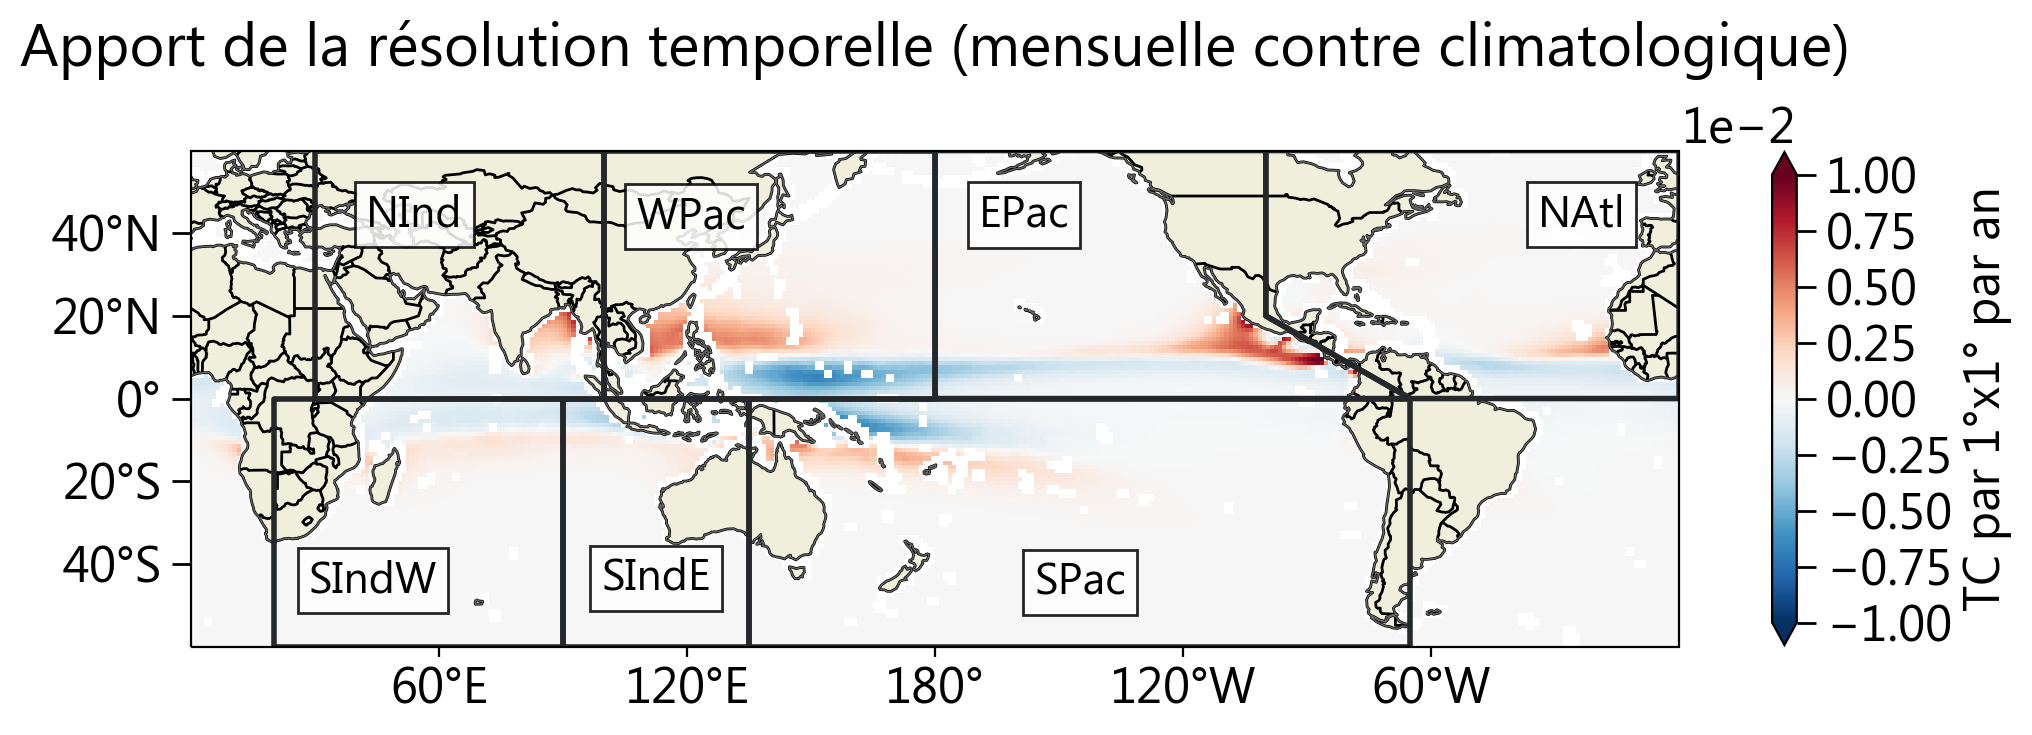
\includegraphics[width=\textwidth]{Figures/apport_mensuel.png}
            \end{figure}
            %
            \vspace{-0.8em}
            \begin{figure}
                \raggedleft
                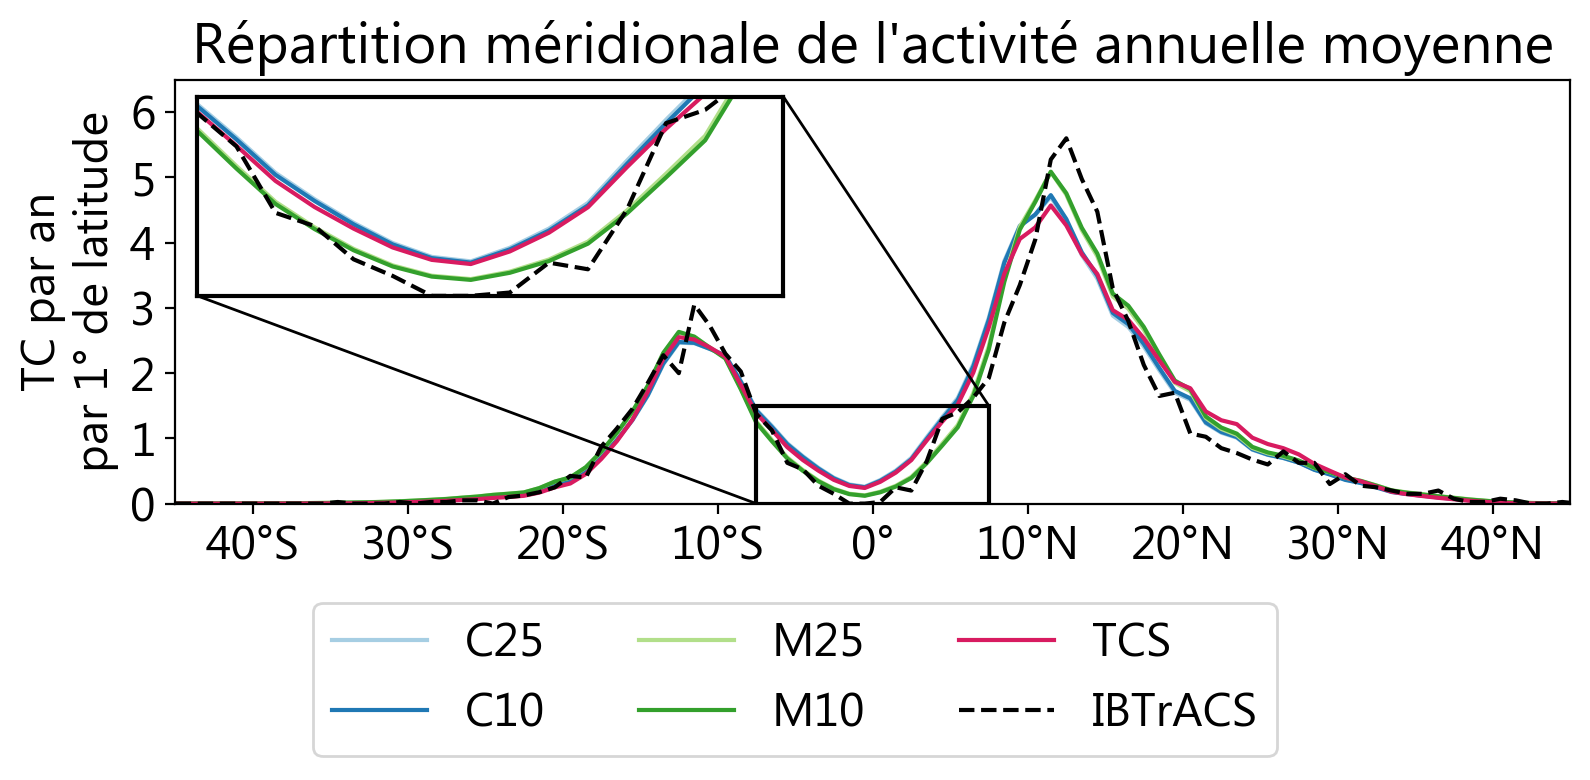
\includegraphics[height=3.5cm]{Figures/zonal.png}
            \end{figure}
        \end{column}
    \end{columns}
    %\vspace{1em}
    %Possiblement sous forme de tableau ?\\
    %$\longrightarrow$ La (mauvaise) représentation de variabilité interannuelle est en fait très robuste aux coefficients
\end{frame}

%=========================================================
\subsection{Prédicteurs utilisés dans la régression}
\begin{frame}[t]
    \frametitle{Ajout d'un diagnostique El Niño dans la régression}
    \scriptsize
    \begin{columns}
        \begin{column}{0.38\textwidth}
            \begin{definition}[Simulation historique ARPEGE]
                \setlength{\leftmargini}{2.5ex}
                \begin{itemize}
                    \item Modèle ARPEGE v6.3 (50~km) \parencite{voldoire_evaluation_2019}
                    \item Période 1979 -- 2010
                    \item Forçage HadISST1
                \end{itemize}
                $\longrightarrow$ SST \alert{historique} mais cyclones \alert{fictifs}
            \end{definition}
        \end{column}
        \begin{column}{0.62\textwidth}
            \vspace{-3em} 
            \begin{figure}[htpb]
                \centering
                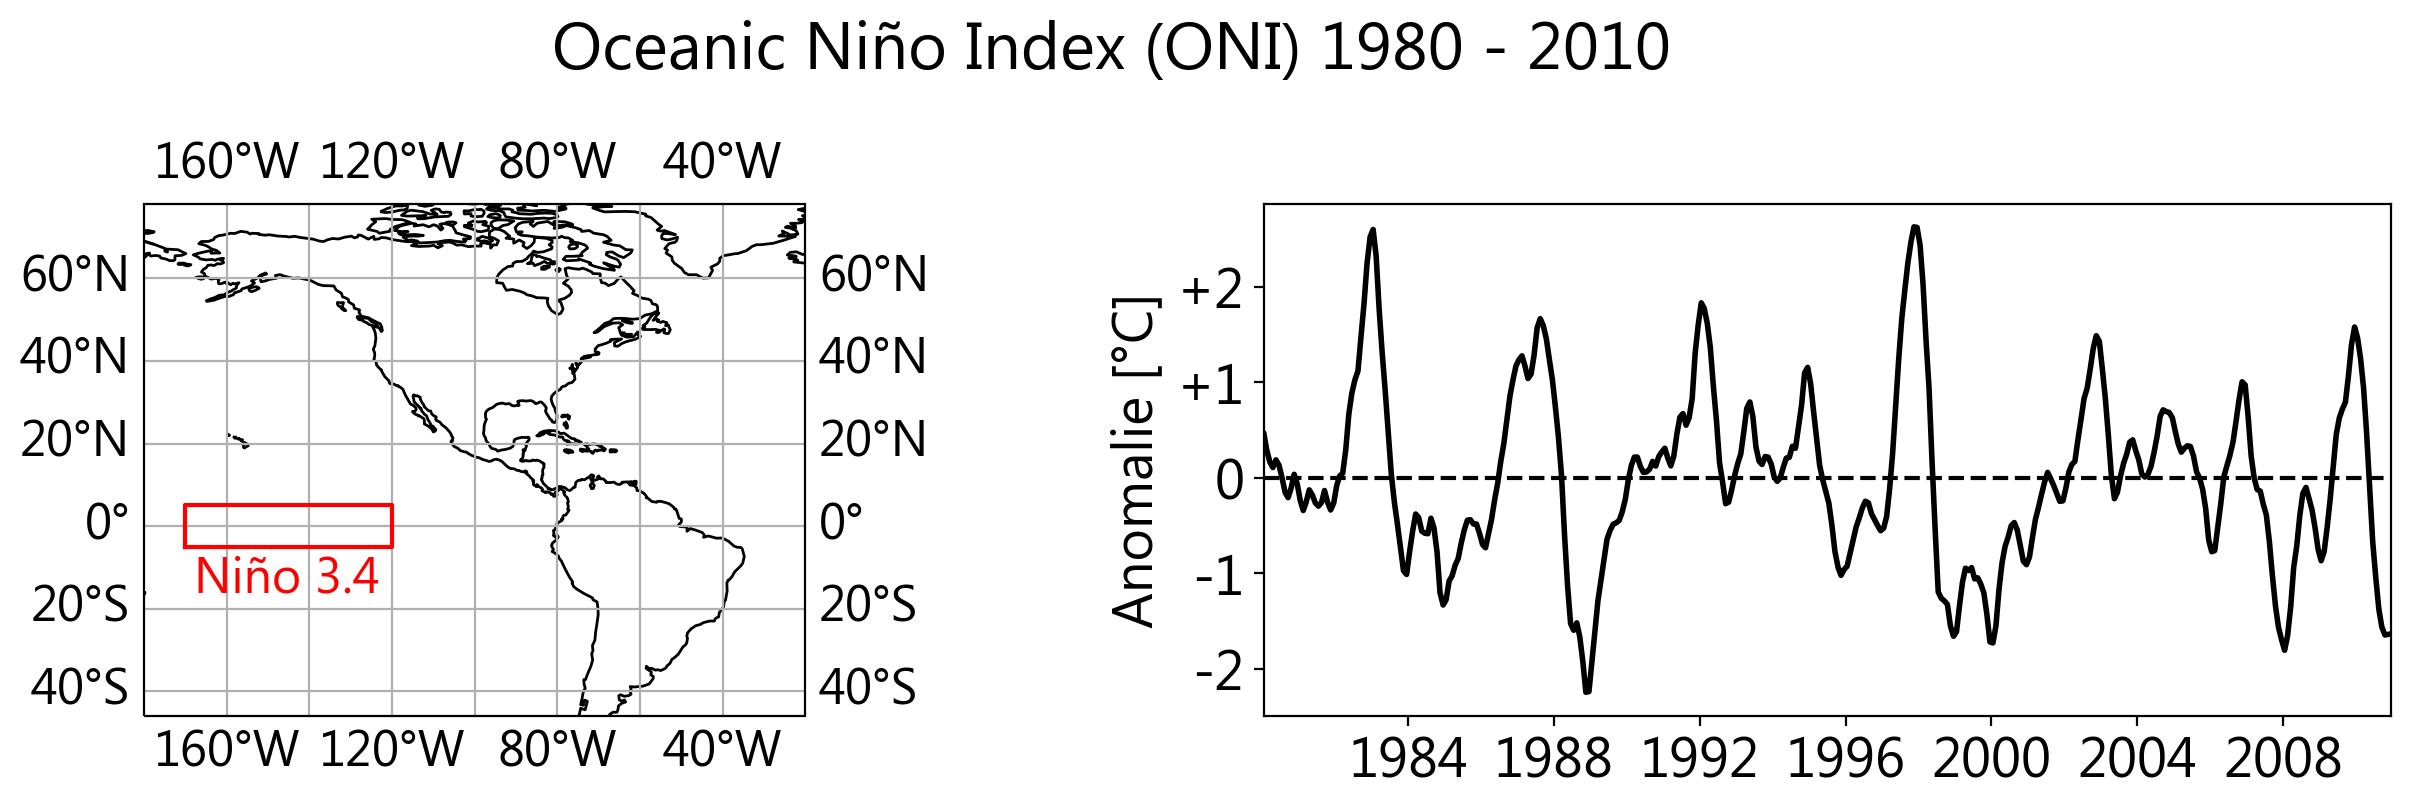
\includegraphics[height=3cm]{Figures/ONI.png}
            \end{figure} 
        \end{column}
    \end{columns}
    %
    \vspace{2em}
    \begin{columns}[t]
        \begin{column}{0.6\textwidth}
            \vspace{-3.5em}%
            \begin{figure}
                \includegraphics<2->[height=4.5cm]{Figures/biais_arpege_correlation_oni.png}
            \end{figure}
        \end{column}
        \begin{column}{0.4\textwidth}
            %\vspace{1em}
            \onslide<3->{
                \begin{examples}[Méthodologie]
                    \setlength{\leftmargini}{2.5ex}
                    \begin{itemize}
                        \item Trajectoires détectées dans la simulation \parencite{chauvin_future_2020} comme prédictant
                        \item Prédicteurs du TCS ($\eta$, $V_\text{shear}$, $H$, $T$) + ONI \alert{répliqué} en tout point
                        \item Régression faite \alert{localement}, à l'échelle du bassin (LOA, Local / ONI / ARPEGE)
                    \end{itemize}
                \end{examples}
            }
        \end{column}
    \end{columns}
\end{frame}

%=========================================================
\begin{frame}[t]
    \frametitle{Introduction d'un diagnostique El Niño dans la régression}
    \framesubtitle{Résultats}
    \vspace{-1em}
    \begin{columns}
        \begin{column}{0.8\textwidth}
            \begin{figure}
                \centering
                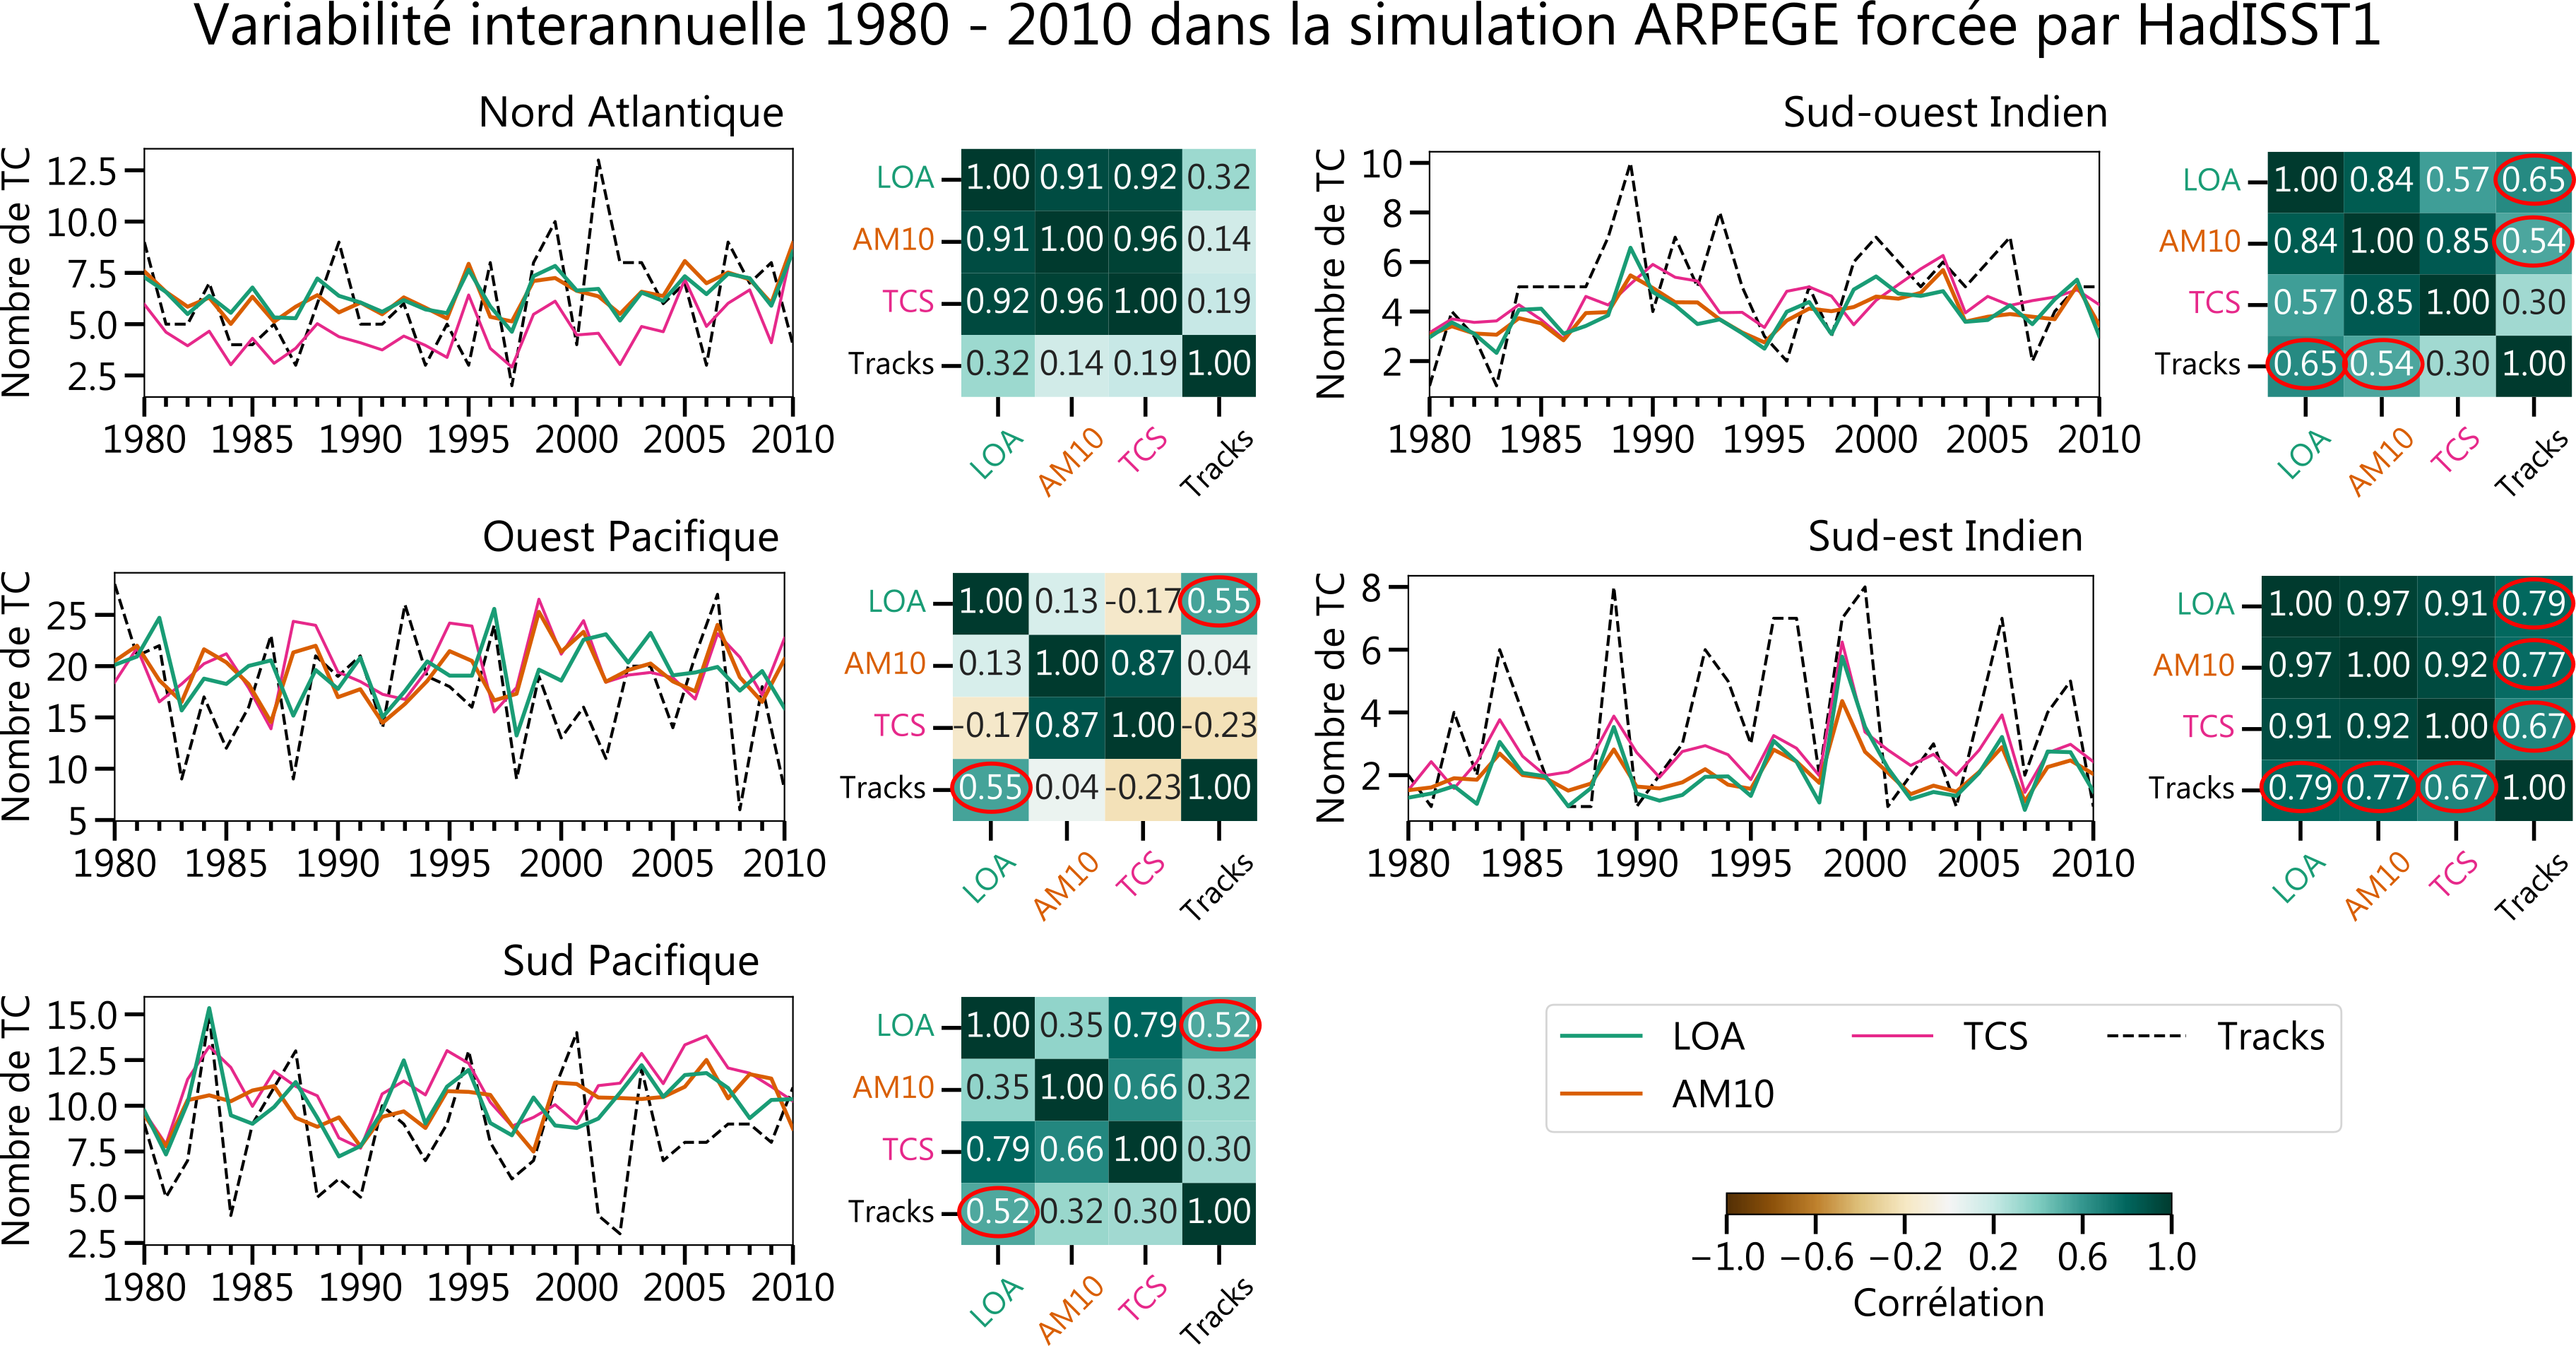
\includegraphics[width=\textwidth]{Figures/apport_ONI.png}
            \end{figure}
        \end{column}
        \begin{column}{0.2\textwidth}
            \scriptsize
            \begin{examples}[Séries représentés]
                \setlength{\leftmargini}{2.5ex}
                \begin{itemize}
                    \item \underline{TCS} :\\Coefficients de \cite{tippett_poisson_2011}
                    \item \underline{AM10} :\\Coefficients du TCS recalculés sur ARPEGE
                    \item \underline{LOA} :\\Indice \alert{local} avec ONI
                    \item \underline{Tracks} :\\Détection et suivi
                \end{itemize}
            \end{examples}
            %
            \begin{block}
                \setlength{\leftmargini}{2.5ex}
                \begin{itemize}
                    \item Ouest Pac. et Sud Pac. Significatifs avec ONI 
                    \item Impact le plus grand pas là où on pouvait l'attendre
                \end{itemize}
            \end{block}
        \end{column}
    \end{columns}
    %
    \onslide<2->{
        \scriptsize
        \begin{center}
            \begin{minipage}{9cm}
                \begin{alertblock}
                    \centering
                    Régression de Poisson peu adaptée à la représentation de la variabilité interannuelle ?
                \end{alertblock}
            \end{minipage}
        \end{center}
    }
\end{frame}

%=========================================================
\begin{frame}
    \frametitle{Déficit de saturation d'humidité}
    \framesubtitle{Écart à la saturation en remplacement de l'humidité relative à 600~hPa}
    \small
    \begin{definition}[Déficit de saturation d'humidité (VPD{,} \textit{Vapour-Pressure Deficit})]
        \footnotesize
        \[ \text{VPD} = e_s - e \]
        Avec :
        \setlength{\leftmargini}{2.5ex}
        \begin{itemize}
            \item $e_s$ : pression de vapeur saturante
            \item $e$ : Pression partielle de la vapeur d'eau
        \end{itemize}
        $\longrightarrow$ \alert{Augmente} avec le réchauffement climatique, tandis que l'humidité relative est projetée constante.
    \end{definition}
\end{frame}

%=========================================================
\begin{frame}[t]
    \frametitle{Déficit de saturation d'humidité}
    %\framesubtitle{Résultats}
    \begin{columns}
        \begin{column}{0.7\textwidth}
            \vspace{-1.5em}
            \begin{figure}
                \centering
                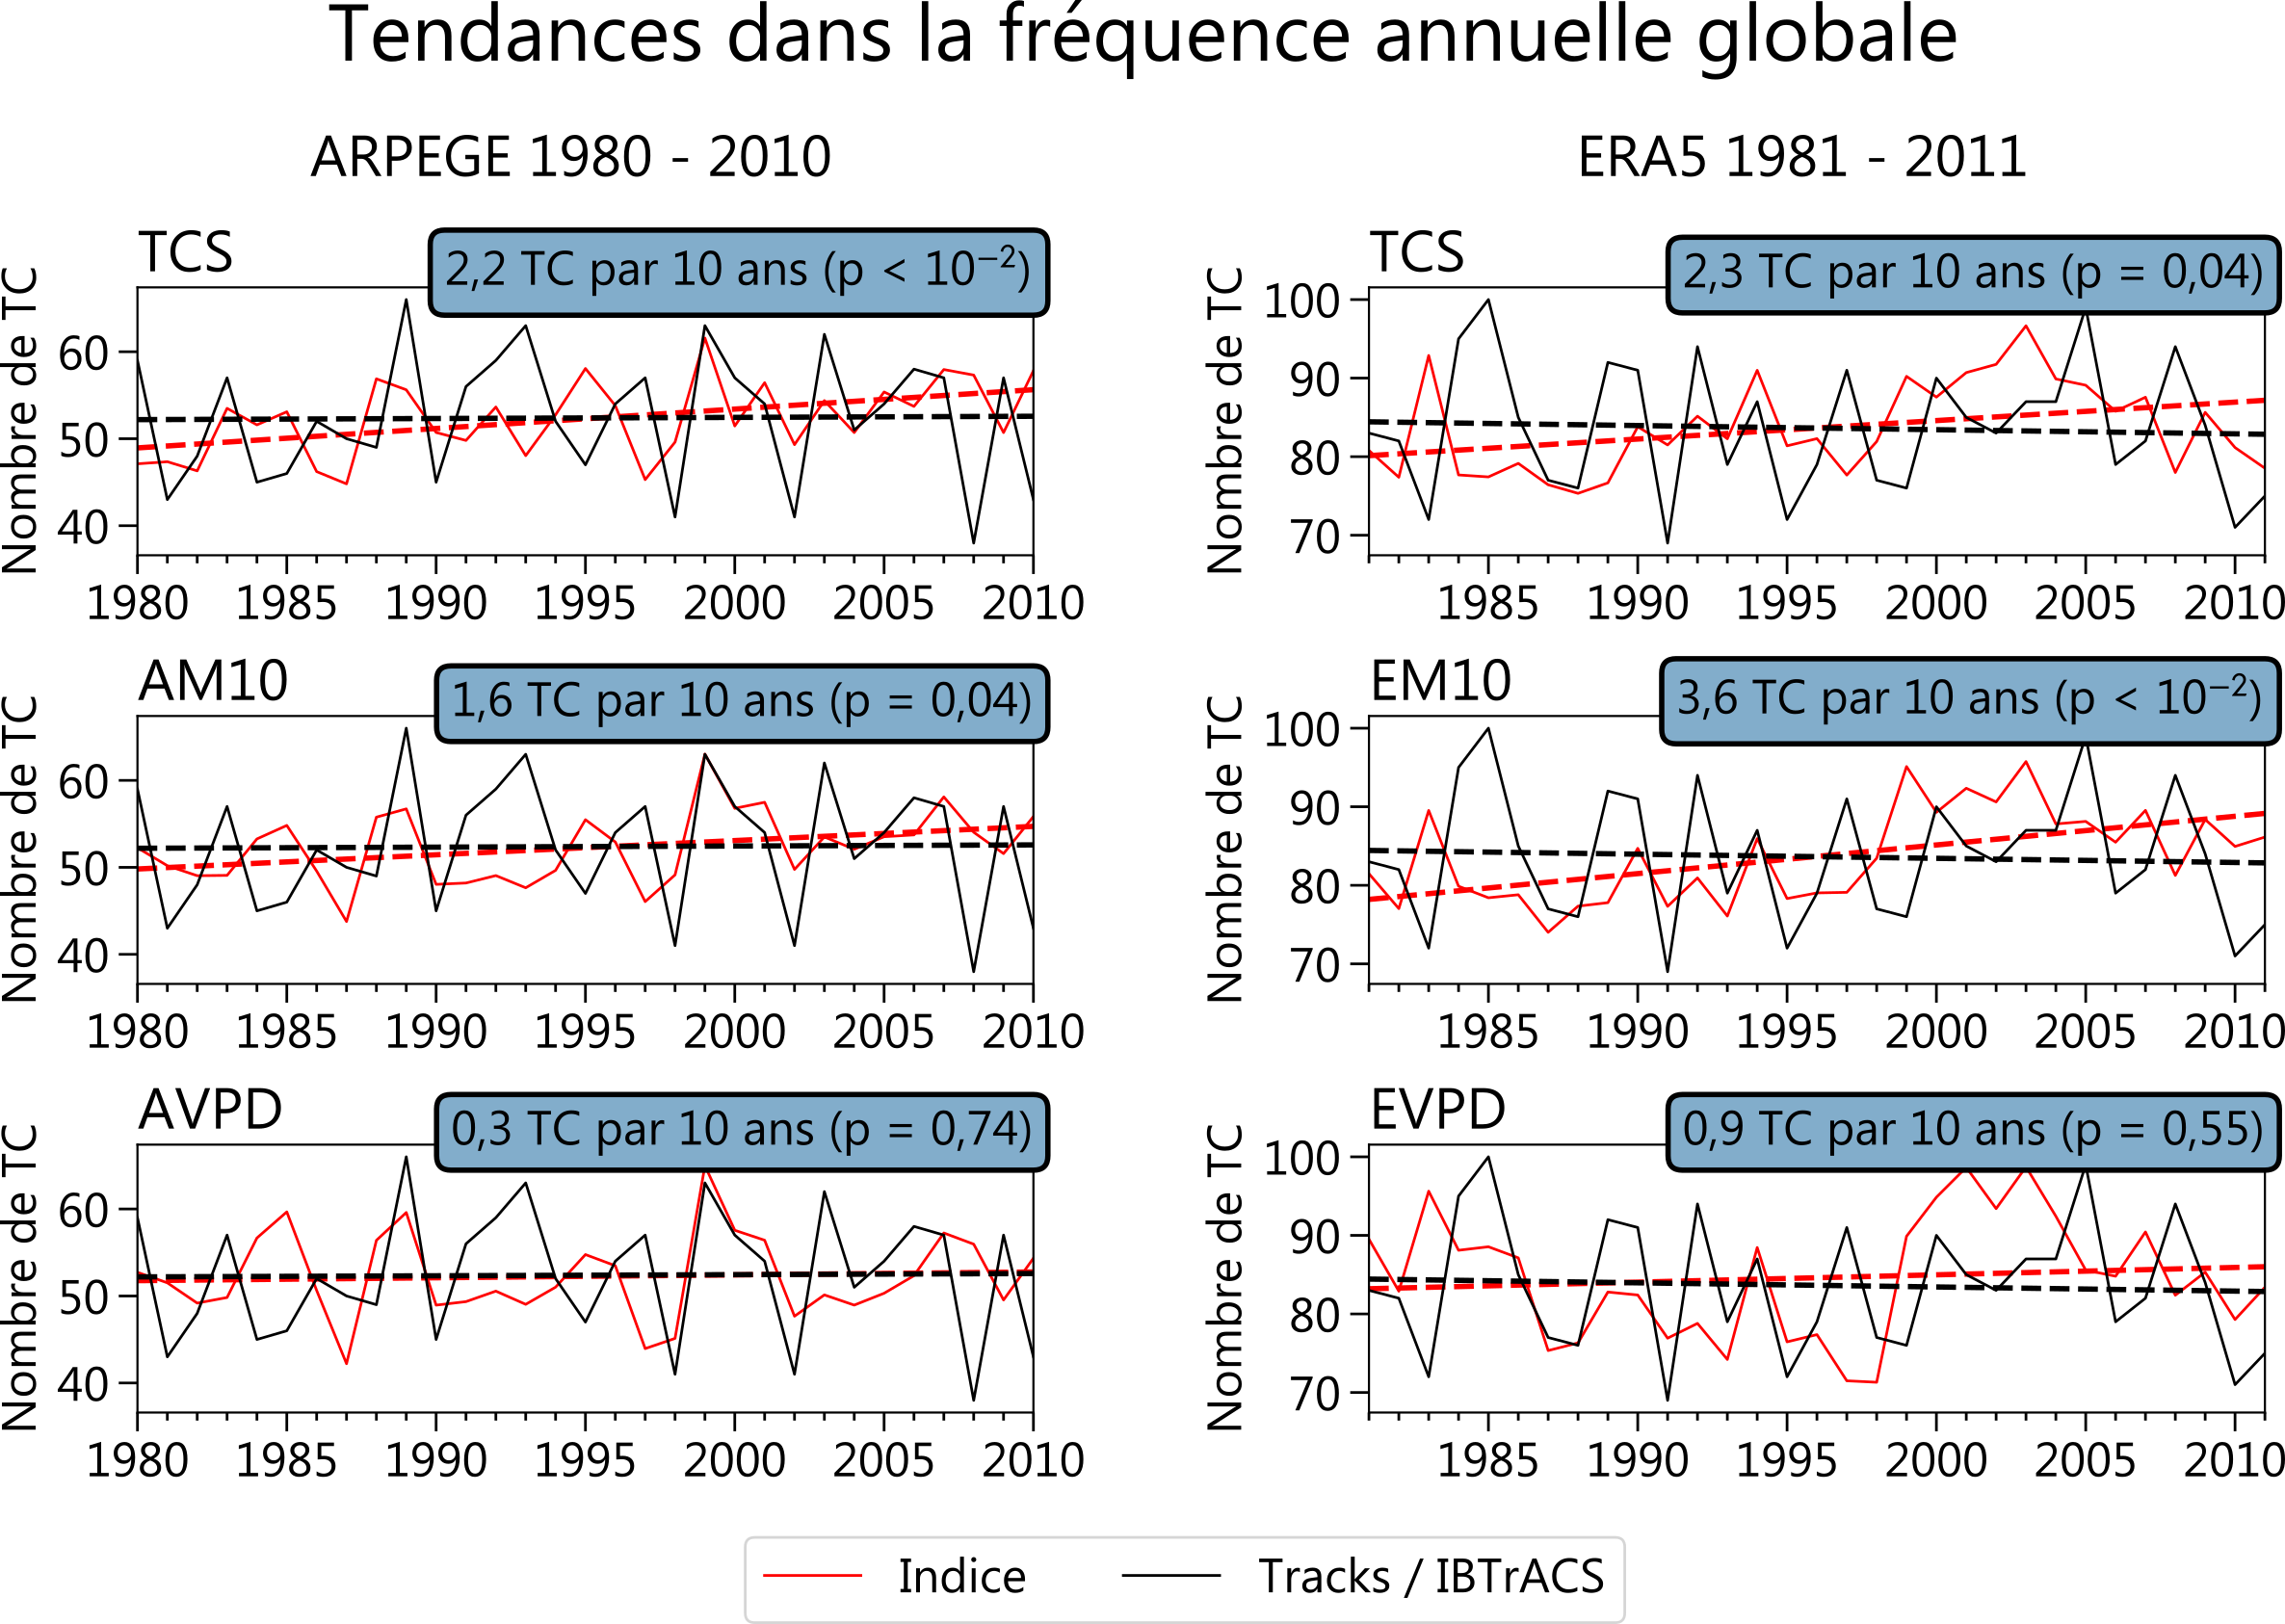
\includegraphics[height=7cm]{Figures/trends.png}
            \end{figure}
        \end{column}
        \begin{column}{0.3\textwidth}
            \scriptsize
            \vspace{-1em}
            \begin{block}[Références]
                \setlength{\leftmargini}{2.5ex}
                \begin{itemize}
                   \item \underline{Tracks} (ARPEGE) :\\
                       0,13 TC par 10 ans (p = 0.9) 
                   \item \underline{IBTrACS} (ERA5) :\\
                        $-0,53$ TC par 10 ans (p = 0.76)
                \end{itemize}
            \end{block}
            \vspace{1em}
            \begin{examples}[Indices]
                \setlength{\leftmargini}{2.5ex}
                \begin{itemize}
                    \item \underline{TCS} : Coefficients de \cite{tippett_poisson_2011}
                    \item \underline{AM10/EM10} : Coefficients du TCS recalculés sur ARPEGE/ERA5
                    \item \underline{AVPD/EVPD} : VPD en remplacement de $H_\text{600~hPa}$ (ARPEGE/ERA5) 
                \end{itemize}
            \end{examples}
            \vspace{1em}
            \begin{alertblock}
                \centering
                Tendances annulées avec le VPD
            \end{alertblock}
        \end{column}
    \end{columns}
\end{frame}

%=========================================================
\begin{frame}[c]
    \frametitle{Synthèse}
    \framesubtitle{Synthèse}
        Synthèse de la partie indice 
\end{frame}

%=========================================================
\section{Conclusion et perspectives}
\begin{frame}[c]
    \frametitle{Conclusion}
    \framesubtitle{Conlusion sur la thèse en général}

\end{frame}

%=========================================================
\begin{frame}[t]
    \frametitle{Conclusion}
    \framesubtitle{Perspectives}
    \begin{itemize}
        \item Foo
        \item Bar
    \end{itemize} 
\end{frame}


%\section*{Bibliographie}
%
%\begin{frame}[t,allowframebreaks]{Bibliographie}
%    \printbibliography
%\end{frame}

%=========================================================
\appendix
\section*{Annexes}
\subsection*{Optimisation du schéma de détection}

\begin{frame}[c]
    \frametitle{Optimisation des paramètres de détection}
    \framesubtitle{Étude de sensibilité du traqueur à ses paramètres}
    \begin{figure}
        \centering
        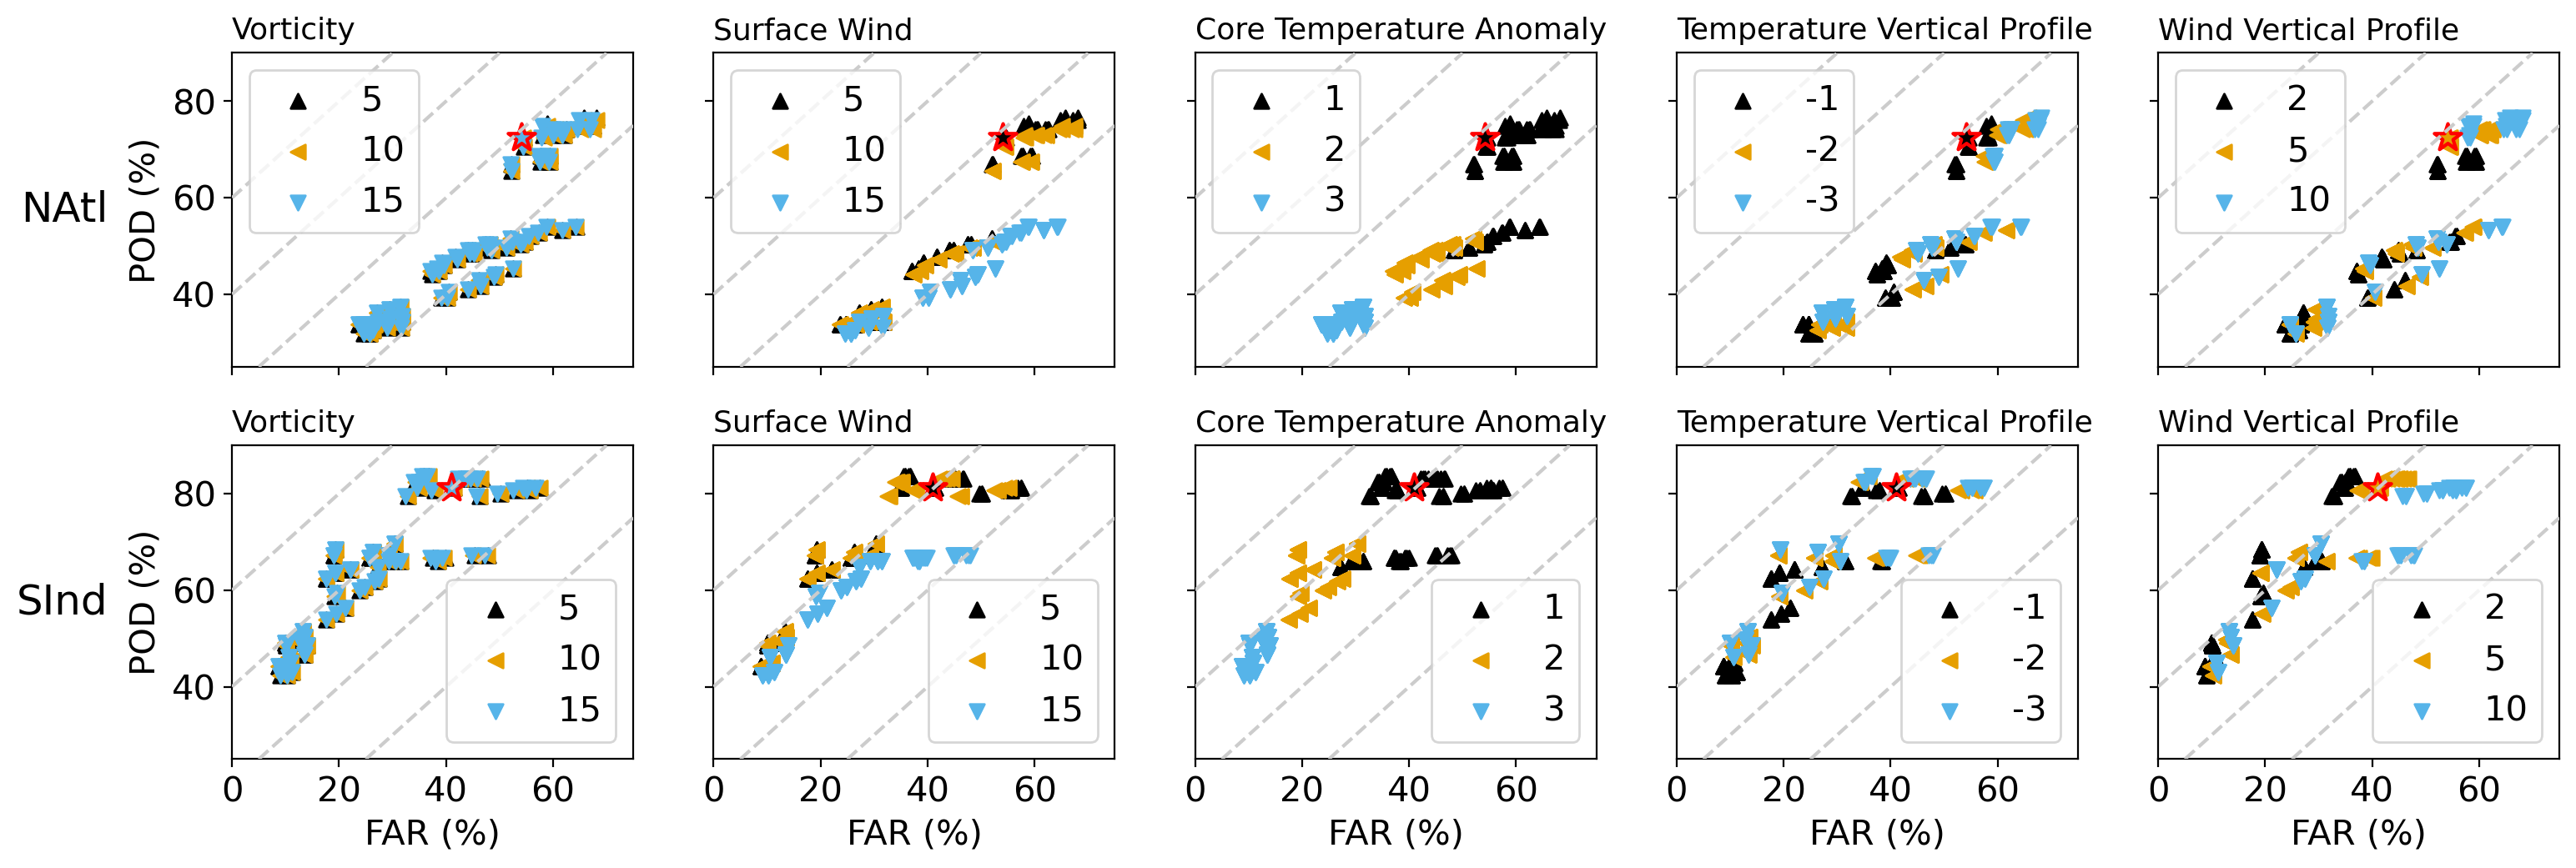
\includegraphics[width=\textwidth]{Figures/optimisation_vectors.png}
        \caption{\small Sensibilité des paramètres du traqueur en termes de FAR et POD sur les bassins NAtl et NInd entre 2008 et 2018. Chaque point correspond
        à une combinaison de 5 paramètres (243 au total).}
    \end{figure}
\end{frame}

%=========================================================
\subsection*{Représentation des TC dans ERA5}
\begin{frame}[t]
    \frametitle{Classes d'intensité croisées}
    \framesubtitle{Contingence par bassin océanique}
    \begin{columns}
        \begin{column}{0.85\textwidth}
            \begin{figure}
                \centering
                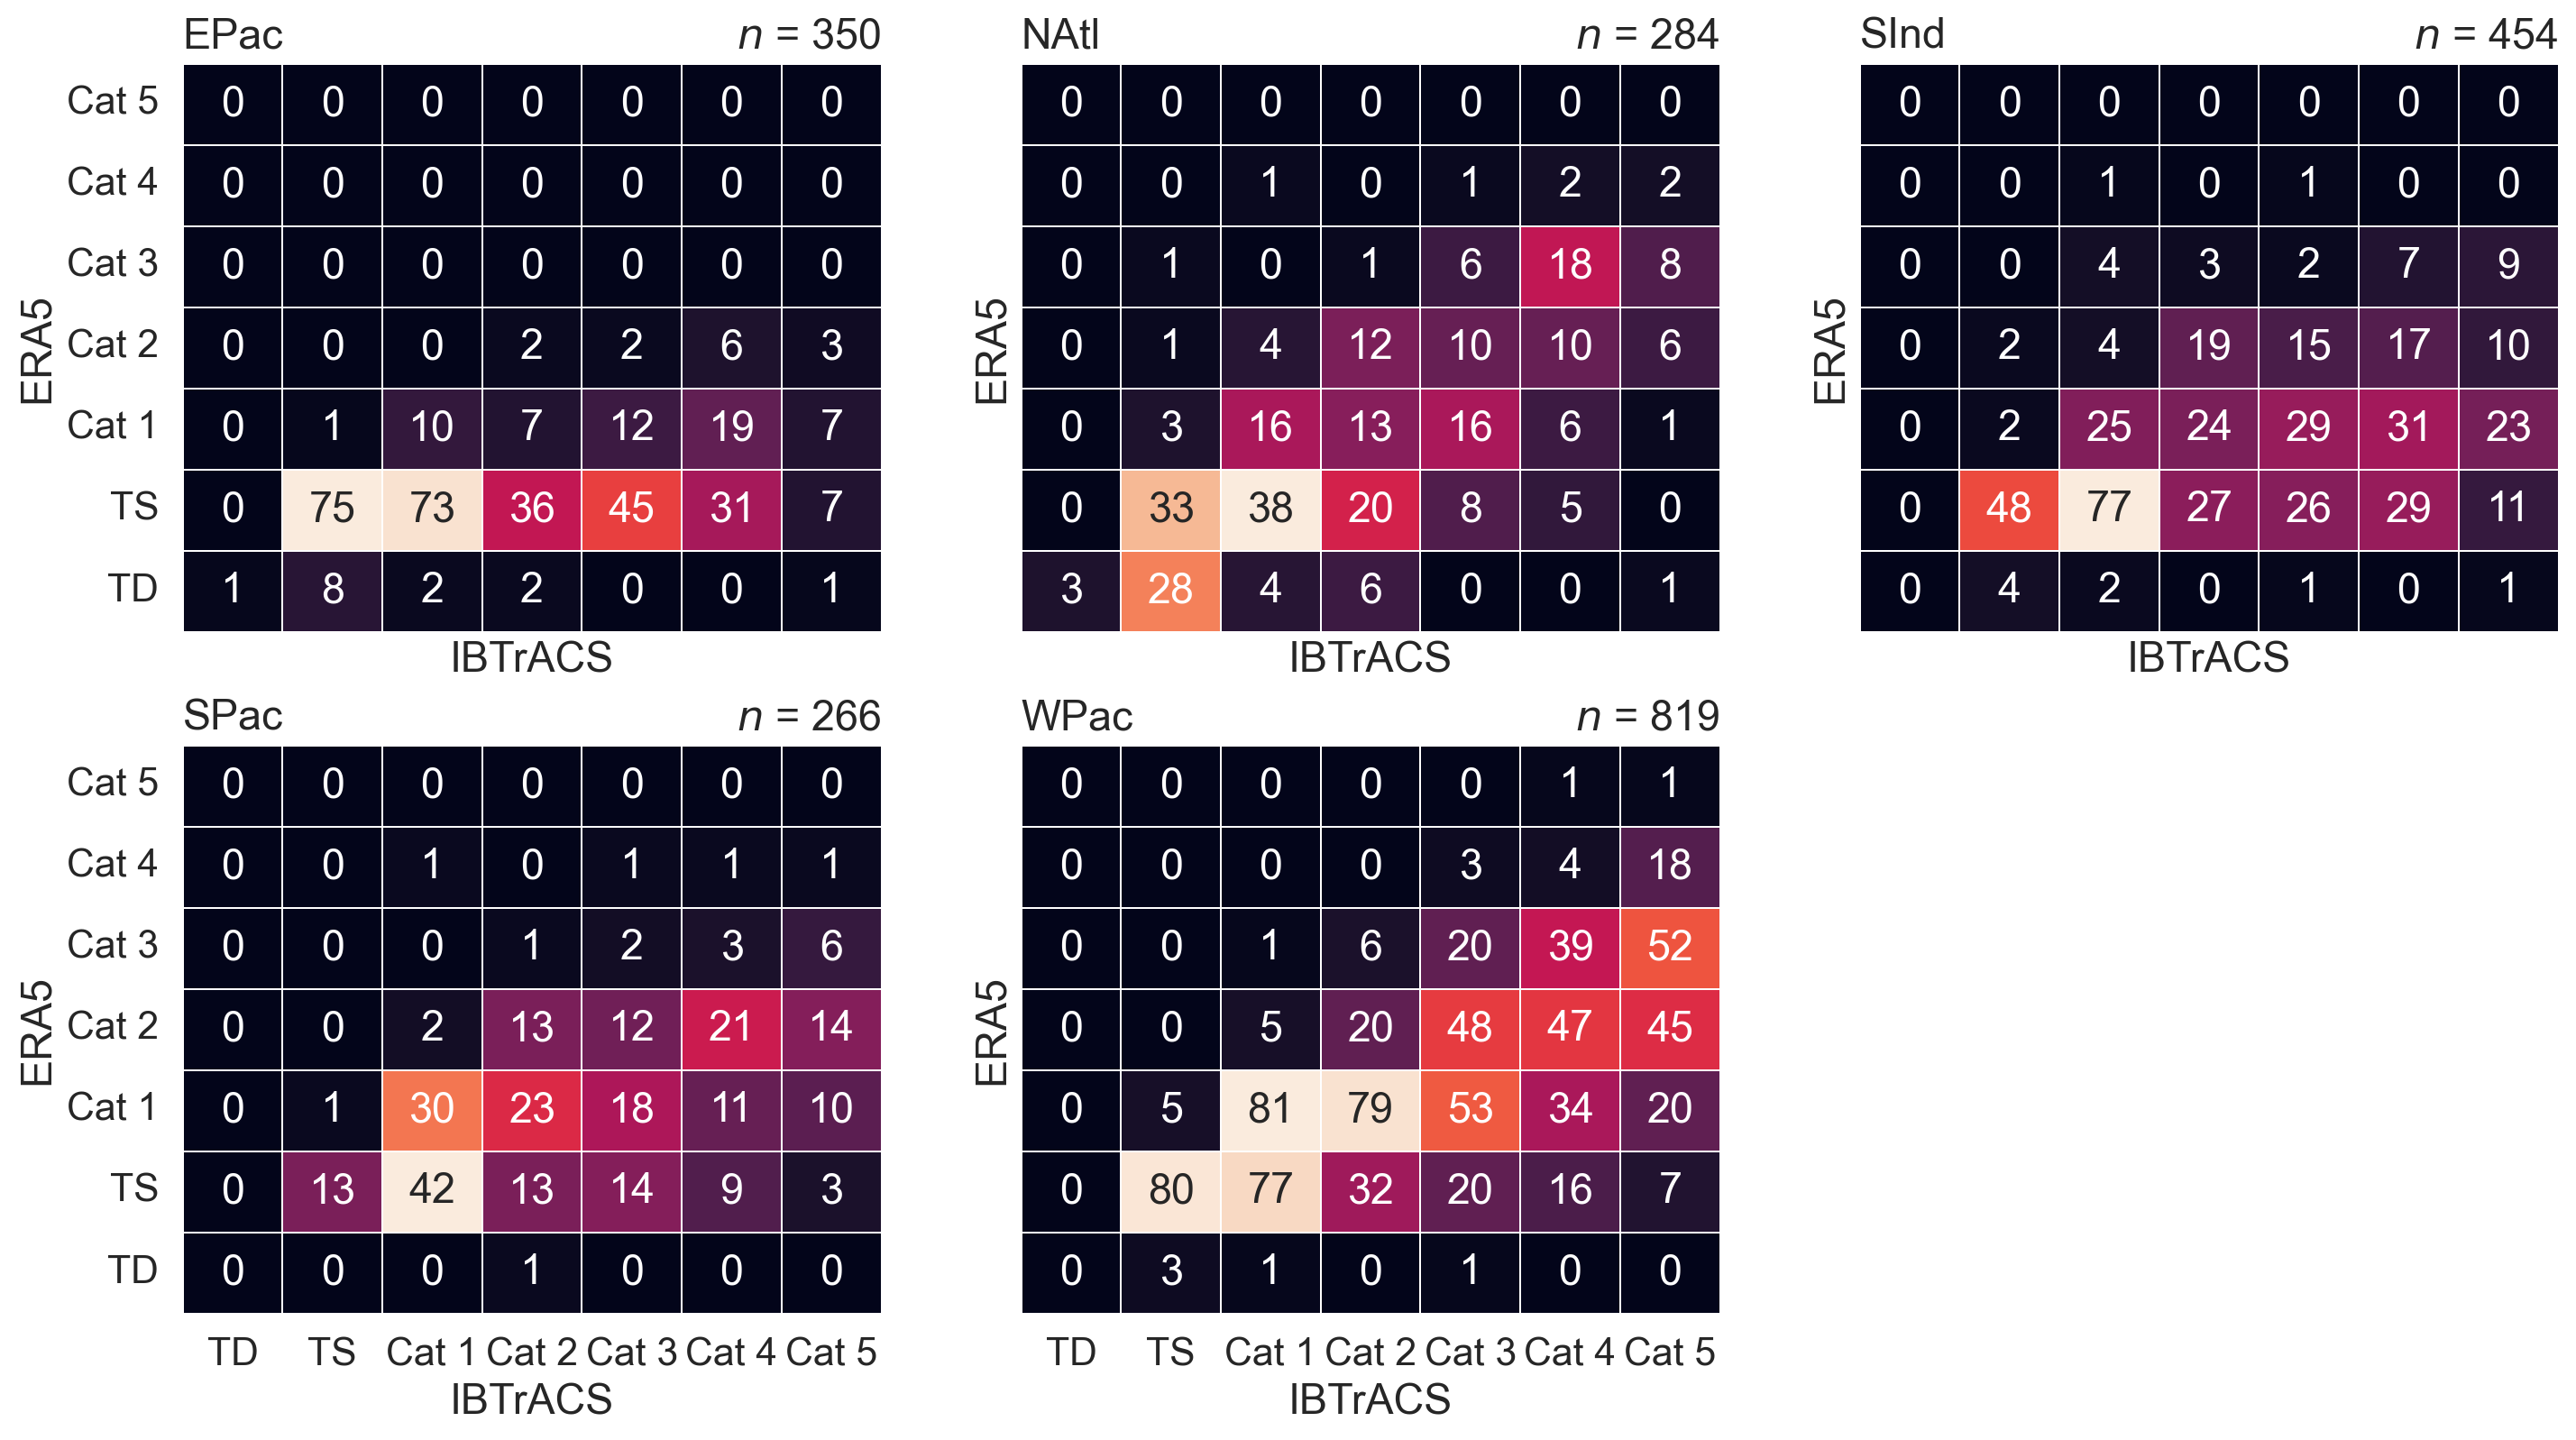
\includegraphics[width=\textwidth]{Figures/Annexes/crosstable_region.png}
            \end{figure}
        \end{column}
        \begin{column}{0.15\textwidth}
            \scriptsize
            \begin{block}
               Relation et dispersion variable selon les régions 
            \end{block}
        \end{column}
    \end{columns}
\end{frame}

%=========================================================
\begin{frame}[t]
    \frametitle{Composites de la structure interne des TC dans ERA5}
    \begin{figure}
        \centering
        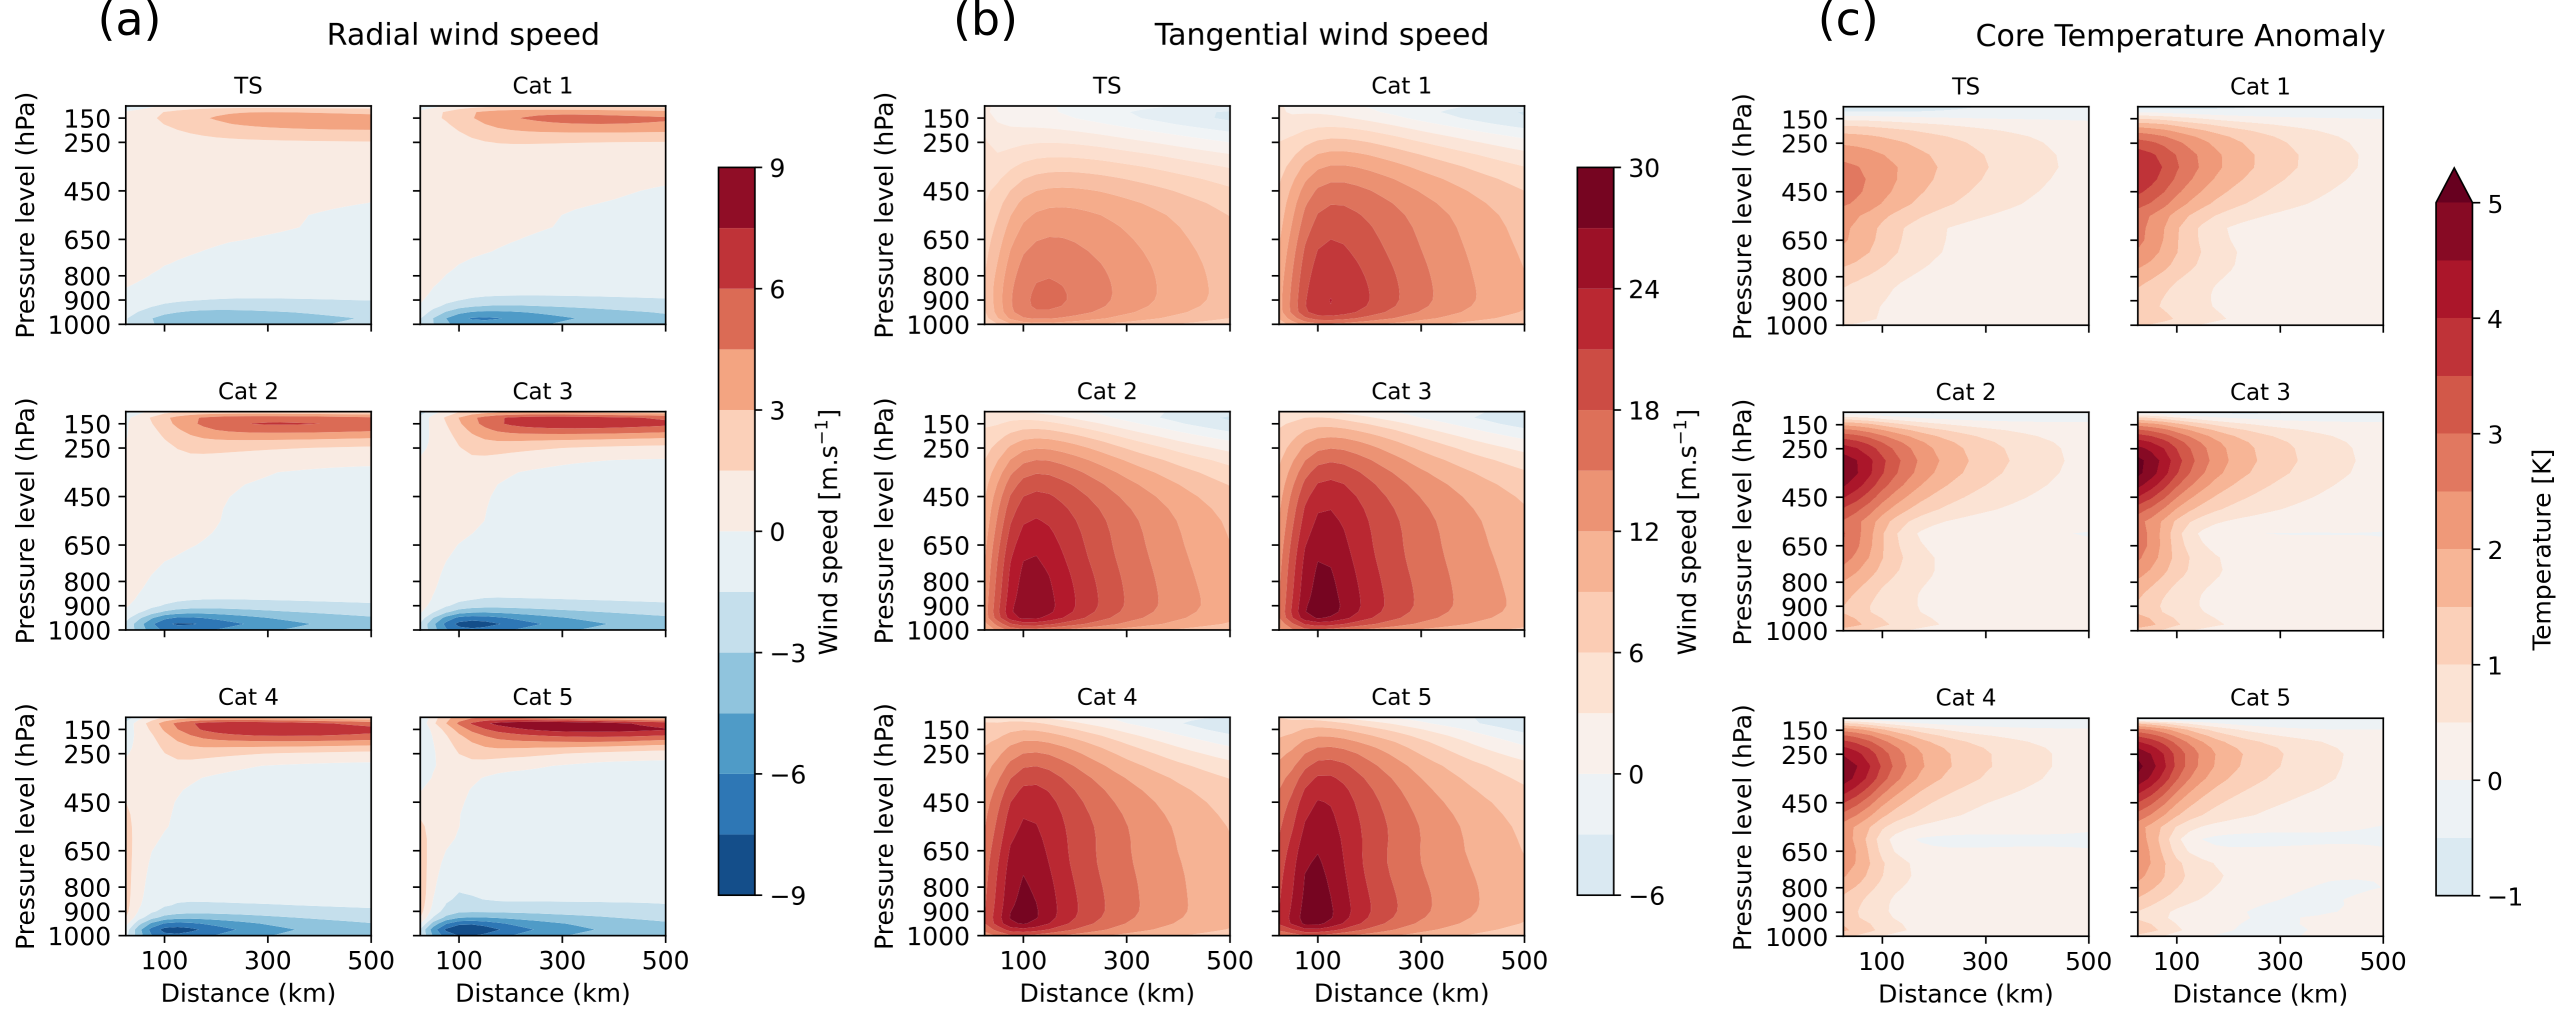
\includegraphics[width=\textwidth]{Figures/Annexes/all_composites.png}
        \caption{\small Composites ERA5 moyennés par classe d'intensité de la composante IBTrACS, indépendamment de l'intensité dans ERA5.}
    \end{figure}
\end{frame}

%=========================================================
\subsection*{Trajectoires simulation ARPEGE historique}
\begin{frame}[c]
    \frametitle{Densité de cyclogénèses détectées dans la simulation ARPEGE historique}
    \begin{figure}
        \centering
        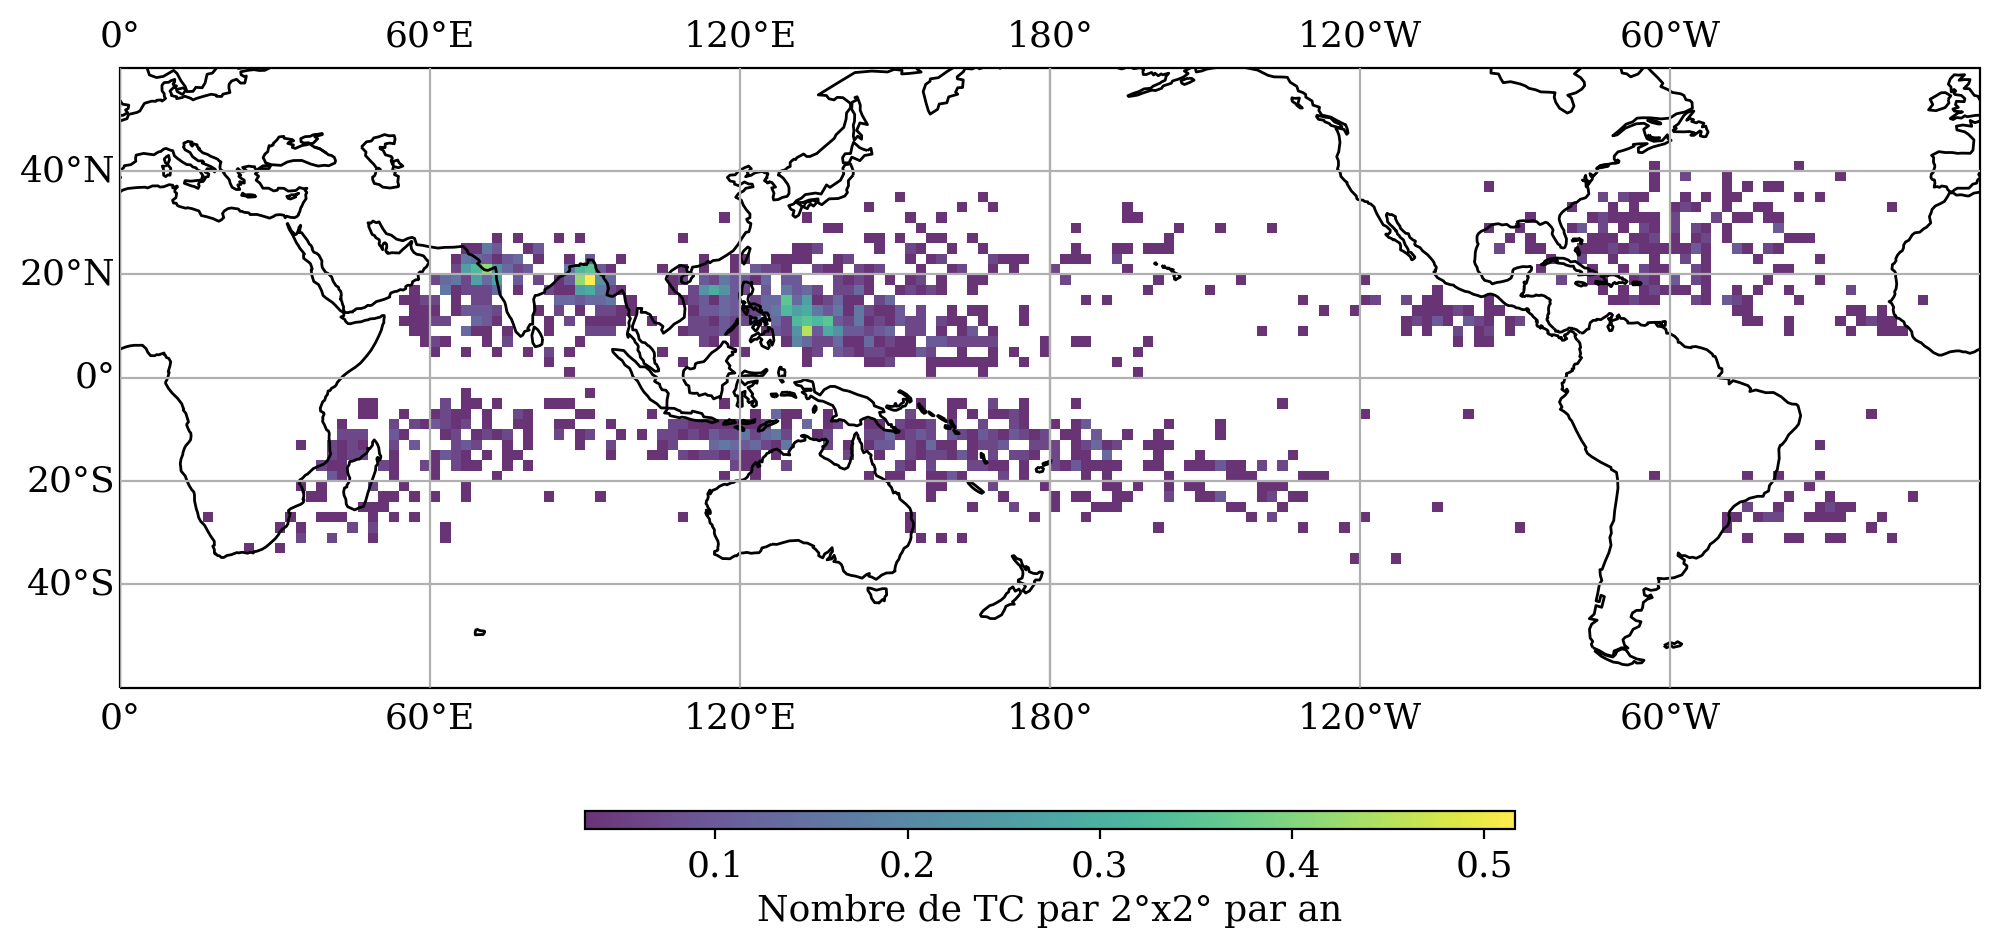
\includegraphics[width=0.8\textwidth]{Figures/Annexes/track_density_PRE625REFT359x.png}
        \caption{\small Densité annuelle moyenne de cyclogénèses dans la simulation ARPEGE forcée par HadISST1 entre 1980 et 2010, calculée sur une grille régulière de 2°×2°.}
    \end{figure}
    
\end{frame}

\subsection*{Ajout de l'ONI dans la régression de Poisson}
\begin{frame}[c]
    \frametitle{Corrélation cyclogénèses détectées avec l'ONI}
    \framesubtitle{Par point de grille}
    \begin{figure}
        \centering
        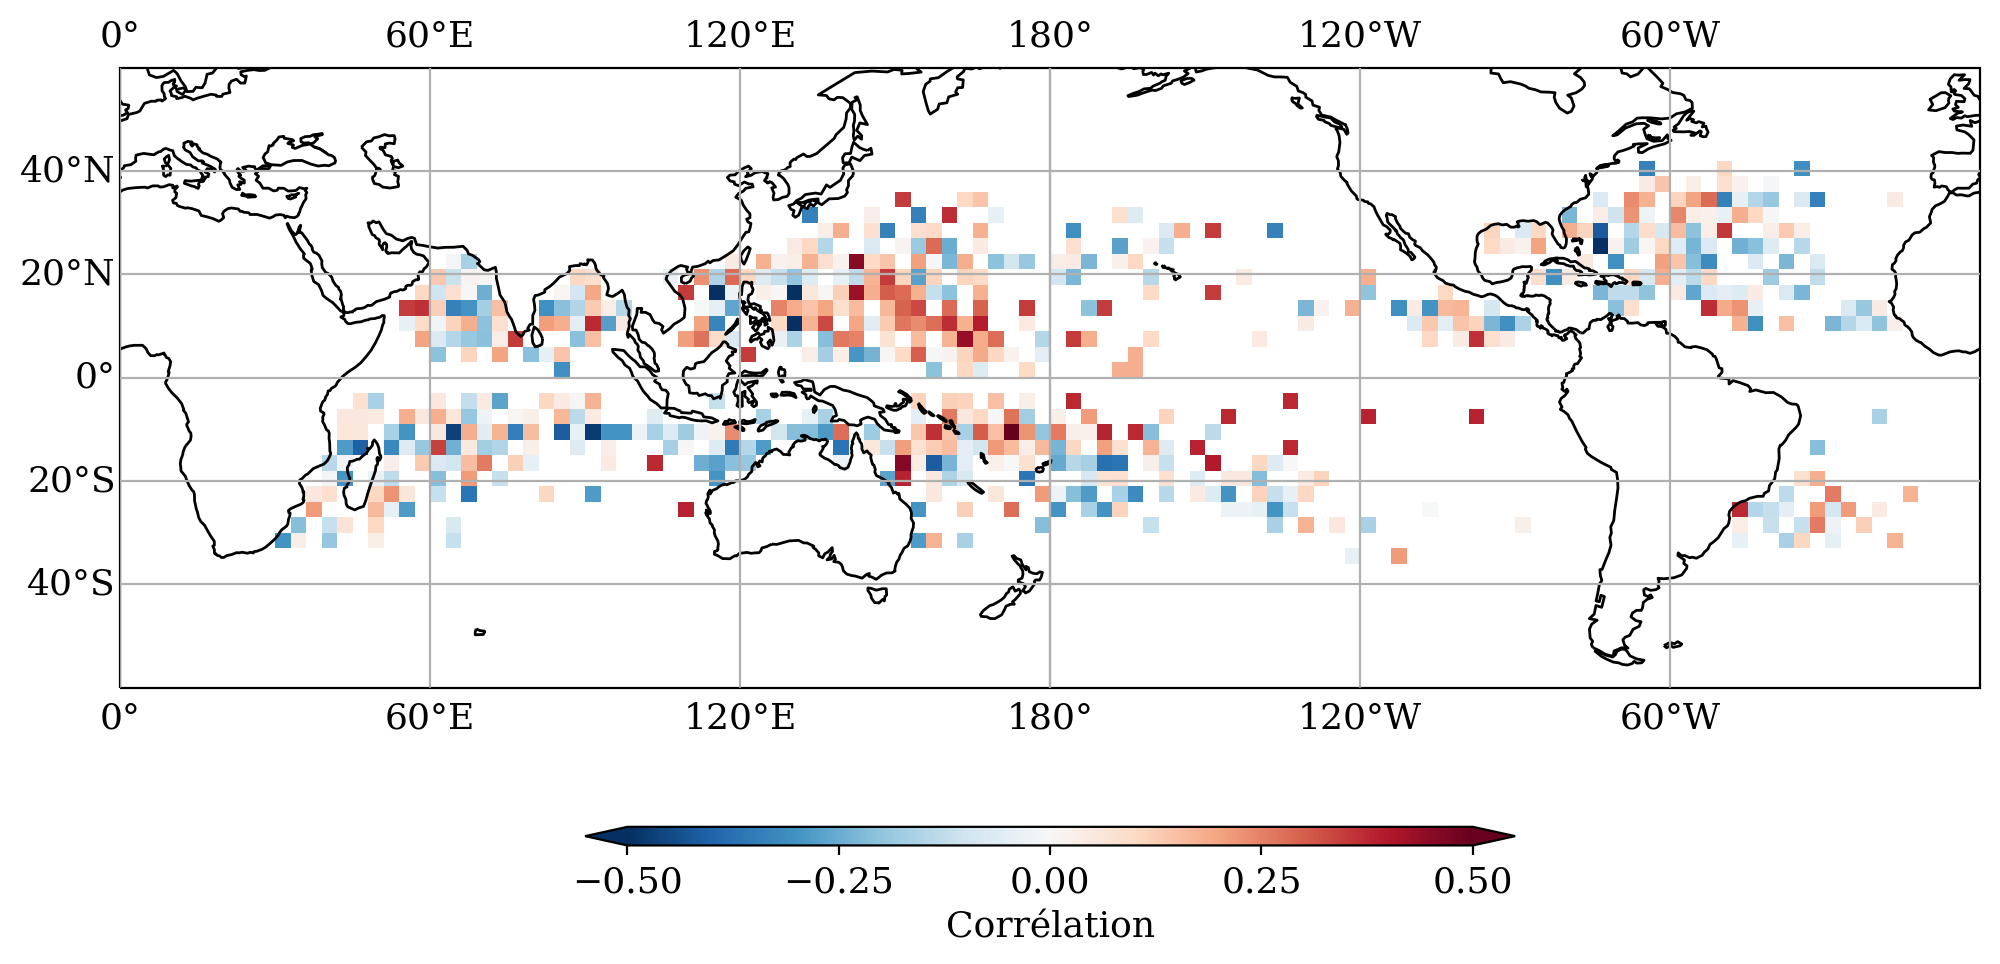
\includegraphics[width=0.8\textwidth]{Figures/Annexes/corr_ONI_tracks.png}
        \caption{\small Carte de corrélation entre la variabilité interannuelle de l’activité cyclonique par point de grille (3 °x3 °) pour les cyclogénèses détectées dans ARPEGE et l’ONI, sur les saisons cycloniques entre 1980 et 2010.}
    \end{figure}
\end{frame}

\end{document}
